
%-----------------------------------------------------------------------------
% Template for AIMS Structured Masters Research Project
%
% The fonts, linespacing, numbering, page styles, order
% of  Title/Abstract/TOC/Body/{Appendices}/Acknowledgements/References 
% are prescribed as the AIMS house style.
%
% Do not change them or add to it without getting approval first.
% Essays are not accepted if they do not follow house style.
\documentclass{aimsessay}
% \usepackage{etex} % fix for using xy and tikz in the same document
\usepackage[utf8]{inputenc}
\usepackage[T1]{fontenc}
\usepackage{lmodern}
\usepackage[round]{natbib}
\usepackage{amsmath}
\usepackage{amsfonts}
\usepackage{amssymb}
\usepackage{mathtools}
\usepackage{latexsym}
\usepackage{parskip}
\usepackage{color,soul}
\usepackage{float}
\usepackage{enumerate}
\usepackage{tikz}
\usepackage{lipsum}
\usepackage{amsthm}


% Fix spacing before theorem environments
\makeatletter\def\thm@space@setup{%
  \thm@preskip=1.5\parskip \thm@postskip=0pt
  }
%\makeatother
% Reduce space before proof
%\makeatletter
\renewenvironment{proof}[1][\proofname]{\par
  \vspace{-\topsep}% remove the space after the theorem
  \pushQED{\qed}%
  \normalfont
  \topsep0pt \partopsep0pt % no space before
  \trivlist
  \item[\hskip\labelsep
        \itshape
    #1\@addpunct{.}]\ignorespaces
}{%
  \popQED\endtrivlist\@endpefalse
  \addvspace{6pt plus 6pt} % some space after
}

\makeatother
% Reduce spacing around section headings?
%
%-----------------------------------------------------------------------------
% To use external packages for specific needs, 
% get approval before adding them here (they
% should not override general AIMS house style and layout).
%
% Examples:
% 
% Load caption before arabtex
\usepackage{caption} %many figures in one figure (note subfigure and subfig are deprecated) 
\usepackage{subcaption} %many figures in one figure (note subfigure and subfig are deprecated) 
% For Arabic
%\usepackage{arabtex}
%\usepackage{utf8}
%\setcode{utf8}
% For tables:
\usepackage{booktabs} % \toprule, \midrule, \bottomrule
\usepackage{array}    % \newcolumntype
\usepackage{listings}
\usepackage{tcolorbox}

%\usepackage{minted}
% 
% For figures:
\usepackage[below,section]{placeins} % use \FloatBarrier in the body to really force a float somewhere. Please limit use.
% \usepackage{float}  %"H" placement spec, for **really here** (i.e. not float)
%
% For code and algorithms
\usepackage{moreverb}   % \verbatimtabinput
% \usepackage{listings} % more flexible and complicated 
                        % than moreverb and algorithm
% 
% Others
% \usepackage[all]{xy}  %  if you use this uncomment \usepackage{etex} above to fix a conflict with tikz.
% \usepackage{sagetex}
% \usepackage{siunitx} % to typeset numbers, units, align decimals in tables.
% \usepackage{dcolumn} % less flexible but maybe faster than siunitx above.
% \usepackage{mathtools} % More maths, e.g. \mathclap.
%
% Others may be landscape, longtable, algorithm, algorithmic, etc.
% 
% ----------------------------------------------------------------------------
% An AIMS Essay can use the sectioning commands "\chapter", "\section",
% "\subsection". No "\subsubsection", "\paragraph", etc. They are disabled.
% 
% For Theorems and such, use the environments defined here:
% \begin{thm}...\end{thm} (or "lem", "defn", etc)
% 
% We put the number to the left of the Theorem heading.
\swapnumbers 
% 
% Theorems are in italics.
\theoremstyle{plain}
\newtheorem{thm}[subsection]{Theorem}
%
% Rest is not in italics.
\theoremstyle{definition} 
\newtheorem{lem}[subsection]{Lemma}
\newtheorem{cor}[subsection]{Corollary}
\newtheorem{conj}[subsection]{Conjecture}
\newtheorem{pro}[subsection]{Proposition}
\newtheorem{exa}[subsection]{Example}
\newtheorem{defn}[subsection]{Definition}
\newtheorem{rem}[subsection]{Remark}
% 
% If you have no theorems, but a lot of equations, maybe the
% following two lines are good. Beware of corresponding Equation
% and Example numbers though! Number equations by sections.
% 
\numberwithin{equation}{section}

%
%-----------------------------------------------------------------------------
% Abstracts are usually written in English, with a version in your
% mother tongue underneath.
%
% French, Igbo, Malagasy, etc. students use normal LaTeX
% for special characters, for example \'{e}
%
% Amharic students use LibreOffice to write Amharic,
% export and include a figure.
%
%\begin{RLtext}    
%Here is where the arabic text goes.
%You can just type it with an arabic keyboard
%\end{RLtext}\\
%-----------------------------------------------------------------------------

% Your own command shortcuts can go here
% keep them clearly separate from other sections of the preamble
% It is good style to have only a few of these so that
% we can read one another's code. If you have to many, 
% then your code does not compile in someone else's template easily,
% and it makes it harder to read. These definitions are only
% meant for very often-used commands to save typing; Examples:
%
%\newcommand {\be}{\begin{equation}}
%\newcommand {\ee}{\end{equation}}
%\newcommand {\C}{\mathbb{C}} % Complex
%\newcommand {\Z}{\mathbb{Z}} % Integers
%\newcommand {\R}{\mathbb{R}} % Real
%\DeclareMathOperator{\sech}{sech} % declaring new math operators like \sin.
%  
%-----------------------------------------------------------------------------
% Title & Author
% On this page you must have NO full-word capitalizations, bold, or colour. 
% All AIMS research projects per year have the same title page.
% In English your family name is written last, i.e. Firstname LASTNAME
% English Capitalization, not as in some Francophone countries where
% you write LASTNAME, Firstname.
% Put your AIMS email address only please, for consistency,
% not gmail or some other webmail address.
\title{Machine learning methods for calibrating radio interferometric data}
%\title{Machine learning methods for analysis of behaviour patterns in radio     interferometric data.}
% Your name must be in English Capitalisation with no comma, 
% and the Family name comes last.
\author{
% Then in the MAIN BODY use this:                  
%\beginنووووووسسسسح%
%\end{RLtext}\\
%%%%%%%%%%%%%%%%%%%%%%%%%%%%%%%%%%%
%\begin{otherlanguage}{arabtext}
%شةشىغ
%\end{otherlanguage}\\
%%%%%%%%%%%%%%%%%%%%%%%%%%%%%%%%%%%%%
% Amharic students speak to me about how to add your name in your own alphabet.
% Everything here is prescribed; do not enter bold or ALL CAPS here,
% it will not be accepted.
%Rhodes university \& SARAO \\
% Example1
% Supervised by Professor Barry Green
% University of Stellenbosch, South Africa
% Example2
% Supervised by Doctor Ingrid Rewitzky
% University of Stellenbosch, South Africa
{\small Author: Simphiwe Nhlanhla Zitha} \\
{\small Supervisors: Dr Arun  Aniyan, Prof Oleg Smirnov, Dr Laura Richter
 }\\
{\small Rhodes University \& SARAO, South Africa}
}
\date{{\small 18 December 2018}\\%
  {\scriptsize\it A thesis submitted in fulfilment of the requirements for the degree of Masters of Science in the\\
 Centre for Radio Astronomy Techniques and Technologies\\
Department of Physics and Electronics}\\%
  \vspace{0.5cm}{
\includegraphics[scale=0.3]{images/R.png}}}
%-------------------------------------------------------------------------
\begin{document}
%\selectlanguage{english}
\pagestyle{empty}
\maketitle
% All other files are included via \input. 
% To compile in texmaker while viewing any of those
% without having to switch back, use
%   Options > Define Current Document as 'Master Document'
% To not have to close a PDF, remove viewpdf from quickbuild 
% and open the PDF (once) manually: it will auto-refresh or with control-r
% 
%-------------------------------------------------------------------------
% The abstract is the first thing we want to see. No acknowledgements or 
% dedications here. Fetch the abstract from a separate file.
% Please write it in English and in your mother tongue.
% An abstract should be less than half a page, so that both abstracts 
% (that is both languages) fit onto one page.
% We number roman numerals until the main body
\pagenumbering{roman}
% Abstracts are usually written in English, with a version in your
% mother tongue underneath
\chapter*{Abstract} 
\addcontentsline{toc}{chapter}{Abstract}


% Don't change anything above this.
The applications of machine learning have created an opportunity to deal with complex problems currently encountered in radio astronomy data processing. Calibration is one of the most important data processing steps required to produce high dynamic range images. This process involves the determination of calibration parameters, both instrumental and astronomical, to correct the
collected data. These parameters include instrumental as well as astronomical parameters. Many astronomers use Common Astronomy Software Applications (CASA) to compute the gain calibration solutions. In this work we present applications of machine learning to first generation calibration (1GC), using the KAT-7 telescope environmental and pointing sensor data recorded during observations. Applying machine learning to 1GC, as opposed to calculating the gain solutions in CASA, has shown evidence of reducing computation, as well as accurately predict the 1GC gain solutions and antenna behaviour. These methods are computationally less expensive and accurate in predicting the 1GC solutions and antenna behaviour. We call this multi-output regression model $\textit{ZCal}$, which is based on random forest, decision trees, extremely randomized trees and K-nearest neighbor algorithms. After the testing and validation of our models, we observe that this model has learned to generalize and predict 1GC solutions with the rms error accuracy at $\approx$ $0.01< rmse <0.09$ for gain amplitude, and $0.2< rmse<0.5$ for gain phase.  
% At a unviersity like Stellenbosch you *must* produce an abstract in Afrikaans for your masters.
% At AIMS you are encouraged to repeat the abstract in your mother tongue
% French, Igbo, Mlagasy, etc. just write it using LaTeX's special
% characters.
% Arabic students see the arabic.tex file for an example
% Amharic use openoffice and export from there and import a figure here.
% Where the words do not exist put the English work in italics, or use mathematical symbols.


% Do not change anything below this except for adding your
% signature (replace images/signature.png) and your name.
\vfill
\section*{Declaration}
I, the undersigned, hereby declare that the work contained in this research project is my original work, and that any work done by others or by myself previously has been acknowledged and referenced accordingly.

% Scan your signature into a small picture called 'signature.png' and insert it
% above your name and the date:
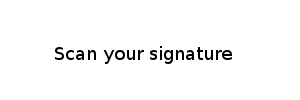
\includegraphics[height=2cm]{images/signature.png} \newline \hrule
% Your name must be in English Capitalisation with no comma, and the Family name comes last. 
% Do note the date below. It is called the "deadline".
Simphiwe Nhlanhla Zitha, 30 May 2018


\chapter*{Acknowledgements} 

I would like to express my sincere acknowledgement to my supervisors: Dr. Arun Aniyan, Prof. Oleg Smirnov and Dr. Laura Richter for their invaluable direction and mentorship.  Prof. Oleg Smirnov who gave me the opportunity to work on this thesis, and introduced me to the SARAO machine learning group. Dr. Arun Aniyan who constantly gave me academic advice and encouraged me to become an independently machine learning thinker. Dr. Laura who helped me to learn the basics of CASA and dealing with KAT-7 data. Thanks to the RATT group for their inputs and comments to this thesis, particular Dr. Sandeep Sirothia who constantly helped me with every questions that are CASA related. I am also very thankful towards the SARAO, my science operations line manager Dr. Lindsay Magnus and science commissioning line manager Dr. Sharmila Goedhart for providing me with learning opportunities and funding to machine learning conferences to present this work.

Last but not least I would also like to thank the God almighty for giving me strength and ability through the course of this thesis. My family  for their continuous support and prayer. My office mates and colleagues Isabella, Sean and Marisa for all the support and reviews of this thesis, Olorato for his continuous support with machine learning and coding. Nkgonne Waka for her prayers and always by my side encouraging and pushing me through the difficulties of this thesis. % Don't go typing out the contents.
\tableofcontents
\newpage
% We switch to arabic numerals here where your page count starts
% Essays must be close to 30 pages long *starting here* and up to and including
% the conclcusion. It does not include the acknowledgements or references.
% 
% Figures may differ between topics, but they are not there
% to fill the pages -- they must add meaning.
% In general most figures should be 0.8 times the width of the page
% (perhaps wider in total when two or three columns of figures)
% See the example in chapter one for defining that. Be *consistent*
% in your presentation of information.
\pagenumbering{arabic}
\pagestyle{myheadings}
%-----------------------------------------------------------------------------
% Each chapter goes in a separate file
% Chapter titles are just examples43w2q1
% Always have a question
% Note the Case Pattern used at AIMS





\chapter*{Preface}

\section*{Chapter 1}
In this Chapter we present the basic introduction to radio astronomy including its history evolving from single dish to interferometry,instruments used to observe the sky, steps undertaken during data processing to correct for the true sky and the importance of the daily "big data" generated by the instruments.    
\section*{Chapter 2}
In this Chapter we present a brief introduction to machine learning and learn its effectiveness in situations where deep and predictive insights need to be uncovered from data sets that are complex and fast changing. how to fine-tune hyper parameters per algorithm used to obtained better results and minimum processing time.  
\section*{Chapter 3}
In this Chapter we describe the machine learning methods and procedure used for the problem, Approach to radio astronomy data processing tools,dataset used for training and testing, how different multi-output predictors respond to complex data set, results.
\section*{Chapter 4}
This brings us to the discussion of the obtained results from the testing and validation data sets.
\section*{Chapter 5}
Finally this brings us to the conclusion and future work plan to improve the performance of our algorithm. 


\chapter*{Publications}

\section*{Conference presentation}

I have been fortunate enough to contribute to the field of Machine Learning and astronomy in the form of an
upcoming academic paper. This work has been presented in prestigious conferences like Neural Information Processing Systems (NIPS) 2017, Machine Learning Summer School (MLSS), Argentina, Buenos Aires, 2018, as well as that of our local Deep Learning Indaba 2017 in South Africa.

NIPS is a machine learning and computational neuroscience conference held being held in every month of December. This is one of the largest and most influential AI conference where researchers gather \citep{NIPS}. 

The MLSS series was started in 2002 with the motivation to
promulgate modern methods of statistical machine learning and inference. This was motivated by the increase in the number of students and researcher who wants to learn about machine learning while there is few machine learning courses that are being taught at universities.
Machine learning summer schools present topics which are at the core of modern Machine Learning, from fundamentals to state-of-the-art practice. The speakers are leading experts in their field who talk with enthusiasm about their subjects \citep{MLSS}.

The Deep Learning Indaba is one of the biggest AI conferences in Africa with the aim to help Africans to participate and contribution to the advances in artificial intelligence and machine learning, and diversity in these fields of science \citep{DLI}. 
 
\chapter{Radio astronomy}



Radio astronomy is one of the most fascinating science fields to study the Universe beyond the immediate vicinity of Earth. Astronomers capture and analyze the electromagnetic signals emitted by distant objects, such as stars and galaxies using a radio telescope. This instrument gather and focus the radiation, revealing information about the evolution and the physics of the Universe. This new window on the history of the Cosmos will reveal the forces that have driven its evolution. In Section \ref{Ra} we present a brief introduction in radio astronomy including the interferometry vs single dish in Section \ref{RvI}. In Section \ref{Calibr} we define calibration in radio astronomy and the different techniques used for data calibration in Section \ref{caltech}. 
\section{Introduction to radio astronomy}
\label{Ra}
\subsection{History}


Radio astronomy is the study of radio radiation from celestial sources emitting at different frequencies  and propagate though space in the form of waves \citep{verschuur2015invisible}. A wave is an oscillatory motion of any kind, the most familiar being waves on the surface of water, sound waves and vibrations of the air or of various material substances. There are also wave disturbances in electric and magnetic field\newtheorem{mydef}{Definition}s. Such waves are responsible for what we experience as X rays, visible light, or radio wave \citep{cassidy2002wave}. The studies of the universe depend on complex instruments to gather the data, including the instrumental properties, advantages, and limitations. Traditional astronomy is based on observations at optical (i.e. visible) wavelengths, but astronomical sources emit radiation not only as visible light but
across the electromagnetic spectrum from gamma rays at short wavelength$(\lambda)$ high frequency $(\nu)$ to radio at long wavelength low frequency as shown in Figure \ref{images/Electromagnetic-Spectrum.png} \citep{staats2016genetic}.

\begin{figure}[h!]
  \centering
    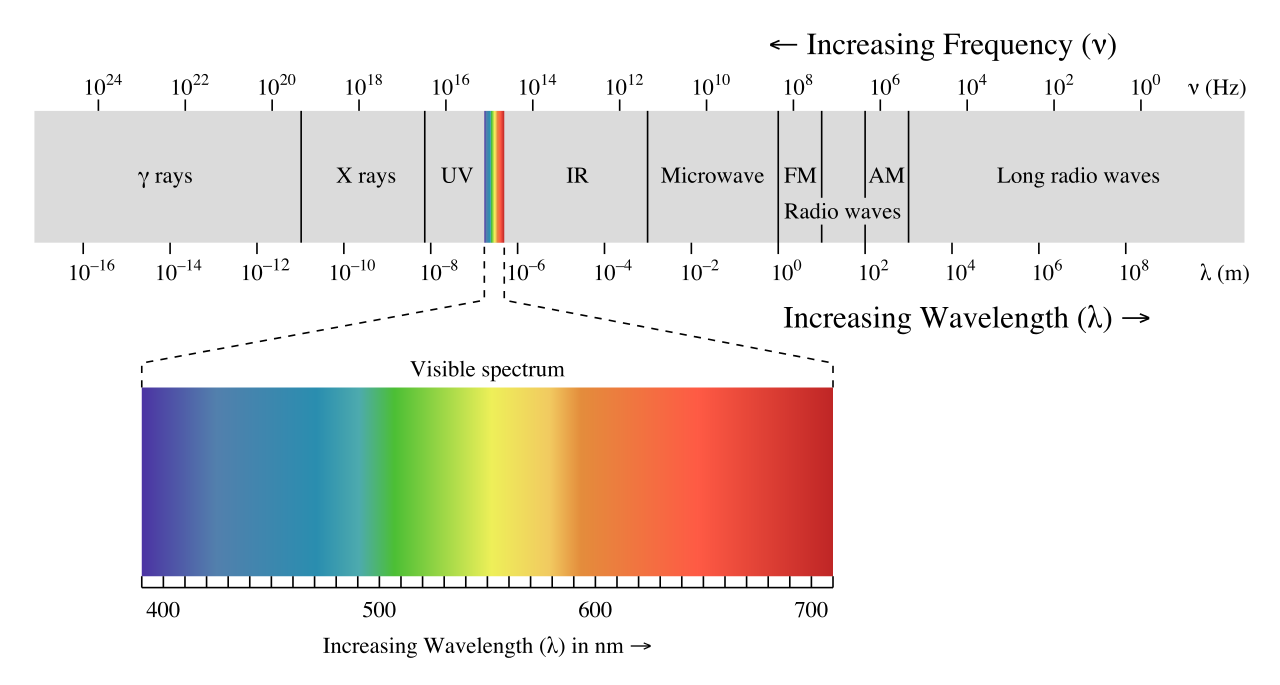
\includegraphics[width=0.7\textwidth]{images/Electromagnetic-Spectrum.png}
    \caption{The electromagnetic spectrum}
  \label{images/Electromagnetic-Spectrum.png}
\end{figure}

Each portion of the electromagnetic spectrum reveals a unique view of the universe and so modern astronomy employs various instruments to look at each portion of the spectrum.\;The Earth's atmosphere absorbs electromagnetic radiation at most infra-red, ultraviolet, X-ray, and gamma-ray wavelengths, so this allow us to only observe the universe from the ground in two windows namely the radio and visible wavebands. Electromagnetic radiation is a group of waves created by fluctuations of electric and magnetic fields radiating/propagating through space at the speed of light ($c=3\times 10^{8} m/s$) carrying electromagnetic radiant energy \citep{staats2016genetic}.\;There are numerous emission mechanisms in the universe that generate radio waves. Radio waves reveals objects that do not radiate in other parts of the electromagnetic spectrum and they are able to pass through galactic dust clouds that obscure the view in the optical range and able to penetrate through the earth's atmosphere (Subject to some limits depending on frequency) \citep{thompson2001interferometry}. After received by a radio telescope, the data is amplified and transferred to a computer (include figure) for further  data processing which is to be discussed in next chapter.


Radio astronomy was accidentally discovered by a radio Engineer for Bell Telephone laboratories, Karl Jansky in the 1930s.
Jansky was assigned the task of investigating the source of radio interference that might interfere with radio-telephone communication system at short wavelengths (10-20 meters) \citep{verschuur2015invisible}.
The purpose of this task was to find out the direction of the radio wave interference so they could easily tune out the interference by using directional antennas pointed away from the direction of the interference. An antenna is a device that receive electromagnetic radio waves and convert them into electrical current. In the process of conducting this task, Jansky constructed an antenna designed to receive radio waves at a frequency of 20.5 MHz (wavelength about 14.5 meters) \citep{Jansky0}. The antenna was mounted of a circular train track so that it could be rotated in all possible angles along the ground and be able to detect radio signal in all possible directions. After several months of recording and analysing these radio signals from all directions, Jansky's investigation became successfully and he identified two known signals (from local and  distant thunderstorms) which were interfering with the radio-telecommunication system, and one unknown signal (faint steady hiss of unknown origin). Jansky continued to investigate the third signal for over a year and he eventually figured out that the radiation was coming from the Milky Way and was strongest in the direction of the center of our Milky Way
galaxy, in the constellation of Sagittarius. This was the first detection of non-black body radiation at radio wavelengths from an extraterrestrial source. Black body radiation is the radiation given off by any object
related to its temperature \citep{Jansky1}.

After Jansky's project at Bell laboratory ended, Bell was not interested in studying astronomy any more. In 1937, an astronomer Grote Reber who was fascinated by Jansky's ground breaking discovery decided to continue where Jansky left off by further investigating the cosmic radio waves from the Milky way Galaxy. To pursue this research, Grote built the first single dish radio telescope with a receiver strong enough to detect radio cosmic signals at the back of his yard, and spent hours at night scanning the sky at different frequencies. A radio telescope intercepts the radiation coming celestial sources and sends the radiant energy it receives through transmission lines. He finally got successfully in detecting radio emission from the Milky Way Galaxy confirming Jansky's discovery \citep{verschuur2015invisible}.   

Astronomical signals tend to be weak by the time it reaches the ground, the need for greater sensitivity and higher resolution has resulted in the focus of new radio telescope development to be in the creation of telescopes that have larger collecting area for more radio energy to be focused on the receiver, external noise minimization and good quality of the receiving system to amplify the signal to levels easier to deal with \citep{verschuur2015invisible}. However constructing a single dish telescope larger enough to achieve high angular resolution $\theta \approx\frac{\lambda}{D}$ (where $\lambda$ is the wavelength of electromagnetic radiation  being observed and $D$ is the aperture diameter of the radio telescope) is physically impossible due to the cost of the materials. The angular resolution of a radio telescope measures its ability to detect fine details in the structure of the observed celestial source. For example, to obtain angular resolution of 1 arc-second, this would require a single dish radio telescope diameter to be appropriately thousands of metres \citep{verschuur2015invisible}. 

\section{Single dish vs Interferometry}
\label{RvI}
Alternatively, a single dish survey can be complemented by an array of small radio telescopes providing higher sensitivity signal and higher resolution images of features initially detected by a single dish survey \citep{wright2004single}. This technique is called radio interferometry, which is basically ensembles of two element interferometers where the incoming radio signal /wavefront from a celestial source arrive at two or more radio telescopes slightly at different times \citep{verschuur2015invisible}. The received signal from each radio telescope is combined with that from other radio telescope in the array as shown in figure \ref{images/Rint.png}. Though the telescopes are separated by distance $b$, the baseline, the resulting output is treated as one telescope. For an interferometric array the angular resolution is $\theta \approx\frac{\lambda}{B}$ where $B$ is the maximum baseline. Single dishes and interferometers  perform similar operation, they provide measurements of the Fourier transform of some region of the sky.

\begin{figure}[h!]
  \centering
    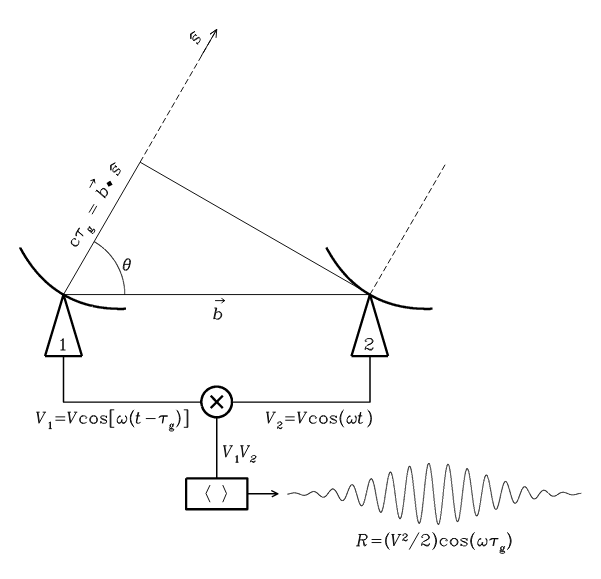
\includegraphics[width=0.45\textwidth]{images/Rint.png}
    \caption{Two antenna interferometer diagram}
  \label{images/Rint.png}
\end{figure}

The figure \ref{images/Rint.png} illustrates a simple two two-element interferometer (we will refer to the left antenna as antenna 1 and the right antenna as antenna 2). This can be extended to multi-antenna arrays by replicating the antenna based portions. For an array of N-elements, there are $\frac{N(N-1)}{2}$ pair of baselines\citep{zensus1995very}. From Figure \ref{images/Rint.png}, suppose a distant star is observed in the sky, If we have two radio telescopes pointing in a direction $\widehat{s}$ at an infinitely far away source, separated by a distance $\overrightarrow{b}$, a  baseline vector from antenna 1 to antenna 2. As the wavefront arrives, it will reach antenna 2 at time $\tau_{g}=\frac{\overrightarrow{b}\cdot\widehat{s}}{c}$ before it reaches antenna 1. $\tau_{g}$ is called the geometric time delay to compensate for the antenna which is further away \citep{taylor1999synthesis}. The output voltages $V_1$ and $V_2$ from both antennas is  denoted by: 

\begin{equation}\label{eq111}
\begin{split}
V_1(t)&=V\cos[\omega(t-\tau_{g})] \\
V_2(t)&=V\cos(\omega\tau_{g})
\end{split}
\end{equation}

$V_1$ and $V_2$ are then  multiplied and time averaged by the correlator to yield an output response whose amplitude R is proportional to the point-source flux density and whose phase depends on the time delay and the frequency.

\begin{align}
V_1 \times V_2 = V^2 \cos(\omega\tau_{g})\times \cos[\omega(t-\tau_{g})]
\end{align}
From $\cos A\cos B= \frac{1}{2} \left(\cos (A+B) + \cos (A-B) \right)$, 
we therefore have 
\begin{align*}
V_1 \times V_2&= \frac{V^2}{2} \left( \cos(\omega\tau_{g} + \omega t-\omega \tau_{g} )\right)\\
&= \frac{V^2}{2} \left(\cos(2\omega t - \omega \tau_{g}) + \cos (\omega\tau_{g})\right)
\end{align*}

We then take the time average $<>$ to remove the high frequency term $\cos(2\omega t - \omega \tau_{g})$ such that we obtain the output 
\begin{align}
R&= <V_1V_2> = \frac{V^2}{2}  \cos (\omega\tau_{g})\\
  &= \frac{V^2}{2}  \cos \left( \frac{\omega}{c} \overrightarrow{b} \cdot \widehat{s} \right)\\
   &= \frac{V^2}{2}  \cos \left( \frac{2\pi \nu}{c} \times
   \overrightarrow{b} \cdot \widehat{s} \right). 
\end{align}

The amplitudes $V1$ and $V2$ are proportional to the electric field produced by the  source multiplied by the the voltage gains of antennas 1 and 2.  Thus the output amplitude $\frac{V^2}{2}$ is proportional to the point-source flux density $S$ multiplied by $\sqrt{(A_1, A_2)}$, where $A_1$ and $A_2$ are the effective collecting areas of the two antennas.

From \ref{eq111} 
Radio interferometry has enable astronomers to make measurements of  of fine angular  details including parameters such as intensity, polarization and frequency spectrum \citep{thompson2001interferometry}.

\section{Calibration in radio astronomy}
\label{Calibr}
\subsection{Interferometry Visibility}
In an interferometric array, the measured visibilities  which is the 2-dimensional Fourier transform of the sky's intensity at different baseline coordinates is defined by
\begin{align}
V(u,v)\approx \mathcal{F}\left\{I\right\}(u,v)=\int \int A(l,m) I (l,m)e^{-2\pi i(ul+vm)} dl dm,
\label{Vis}
\end{align}
where $(u,v)$ denotes the projected baseline coordinates in the 2D plane Fourier transform measured in wavelength along axes in the east-west and north south direction,  and changes with time as the earth rotates. $(l, m)$ are the orthogonal coordinates representing the position of a source or the phase reference position. In the 2D analysis $l$ and $m$ are defined as the cosines of the  angles between the direction $(l,m)$ and $(u, v)$. $I(l,m)$ is the intensity distribution of a source and its Fourier transform  ${F}\left\{I\right\}$ represents the amplitude and phase of sinusoidal component of the intensity profile with spatial frequency $u$ and $v$; and and $A(l, m)$ represents the effective collecting area of the antennas with respect to the direction of the incoming radiation.

For simplicity of \ref{Vis}, the term $A(l,m)$ is most often assumed to be 1 such that the Van CittertZernike theorems states
\begin{align}
V(u,v)\approx \mathcal{F}\left\{I\right\}(u,v)=\int \int I (l,m)e^{-2\pi i(ul+vm)} dl dm.
\label{V}
\end{align}
The measured visibilities $V(u,v)$ and the sky brightness I $(l,m)$ are Fourier pairs $V(u,v) \rightleftharpoons I(l,m)$, where $\rightleftharpoons$ is the Fourier transformation. The sky
brightness can readily be recovered from the measured visibilities by an inverse Fourier transform such that we have 
\begin{align}
I(l,m)\approx \mathcal{F}^{-1}\left\{V\right\}(l,m)=\int \int V (u,v)e^{-2\pi i(ul+vm)} du dv.
\end{align}
Since for every sky's brightness $I$ $\exists$ visibility function $V(u,v)$, the array of an antennas with baseline $b=(u_i,v_i)$  measures only a certain values in the $\textbf{Set}$ of continuous  $(u,v)$ in the visibility function $V(u,v)$. This measured set of values is called \emph{Sampling function} denoted by \citep{taylor1999synthesis} \[ S(u,v) =
  \begin{cases}
    1   & \quad    \text{at uv point}\\
    0  & \quad  \text{ otherwise}\\
  \end{cases}
\], $\forall$ baselines. The actual data provided by the array is called  sampled visibilities denoted by  $S(u,v)\times V(u,v)$. The Fourier transform of this sampled visibilities is the dirty Image
\begin{align}
I^{D}(l,m)=\int \int S(u,v)\times V(u,v) e^{-2\pi i(ul+vm)} du dv.
\label{Samp}
\end{align} 
Using the $\textit{convolution theorem}$ for Fourier transforms which states that the Fourier transform of the convolution of two functions is the product of their Fourier transforms denoted by 
\begin{align}
f*g\rightleftharpoons \mathcal{F} \mathcal{G},
\end{align}
where $f\rightleftharpoons \mathcal{F}$ and $g\rightleftharpoons \mathcal{G}$.
From \ref{Samp}, we therefore have 
\begin{align}
I^{D}=PSF \circ I^{True},
\end{align}
where 
\begin{align}
PSF(l,m) = \int \int S(u,v)e^{-2\pi i(ul+vm)} du dv,
\end{align}
represents a point spread function  corresponding to the sampling function $S(u,v)$.


\subsection{Calibration}
\label{Calib}
In radio astronomy, ideally one might think that after obtaining the observed visibilities the next step would be to directly retrieve the actual visibilities of the target source and perform imaging. However, in reality case it is not as simple as shown by equation \ref{V}. The measured visibilities $V^{obs}$ are different from the actual visibilities $V^{True}$ not only due to the instrument being discrete as shown in equation \ref{Samp}, but most importantly due to instrumental and environmental effects \citep{abebe2015study}. An example of these effects on the signal measured by a radio interferometry include antenna gains(slowly and fast time-varying instrumental part), atmospheric effects, pointing errors (tracking inaccuracies), Incorrect observation parameters (antenna pointing parameters). Signal effects are classified in two types; direction independent effects (affects signal from all direction of the sky) and direction dependent effects(which vary based on the sky position of the where a signal originated) \citep{taylor1999synthesis}. These effects can be corrected by estimating the errors associated with the measured visibilities, thereby recovering the true visibilities. This process is called calibration. In its simplest form, calibration boils down to minimizing the difference between observed and predicted(model) visibilities by estimating the complex instrumental gain response \citep{grobler2016calibration}. 

Suppose for baseline pair $(i,j)$, the observed visibility is $V^{obs}_{i,j}(t)$ and the true visibility is $V^{True}_{i,j}(t)$ at observation time $t$. The basic calibration formula is written as 

\begin{align}
V_{i,j}^{obs}=G_{i,j} V_{i,j}^{true} + \epsilon_{i,j}(t) ,
\end{align}
where $G_{i,j}(t)$ denote the complex antenna gains for baseline $(i,j)$ as a results of unwanted effects and may vary with time \citep{thompson2001interferometry}. The extra term $ \epsilon_{i,j}(t)$ is a stochastic complex noise \citep{taylor1999synthesis}.

Since most of the corruptions in data occurs before the signal gets correlated and the response associated with antenna  $i$  does not depend on the response of antenna $j$. Then the baseline-based complex gain $G_{i,j}$ can therefore be approximated into the product of amplitude and phase $A$ and phase $\phi$ such that we have  

\begin{align}
G_{i,j}(t)= g_i(t)g^*_j(t) = A_{i}(t)A_{j}(t) e ^{i\left(\phi_i(t)-\phi_j(t)\right)},
\label{Sols}
\end{align}

where  $A_{i}(t)$, $A_{j}(t)$ are antenna-based amplitude solutions and $\phi_i(t),\phi_j(t)$ are antenna-based phase solutions. Calibration means to find the appropriate $A$ and $\phi$ for the corrupted visibilities. One standard technique of obtaining solutions to \ref{Sols} is to obtain dedicated calibration observations of a part of the sky that contains a single known, relatively strong point source. The reason for observing these sources is to measure the instrumental phase since the telescopes on the ground can only measure the phase differences rather than measuring absolute phase reference. Therefore, the reference for phase visibility to the phase tracking center or the center of the primary antenna beam can be practically accomplished by observing point-like calibrator sources, the phase . Using these sources, one can determine the phase deviation from the desired reference point. Periodic observation of these sources is very important so as to track the phase and gain changes in an array. Above all, they have the paramount advantage to estimate time dependent phase changes incurred by the atmosphere \citep{taylor1999synthesis}.

The selection of a good calibrator source in the sky is based on the following desirable characteristics \citep{thompson2001interferometry} 

\begin{enumerate}
\item They should have known positions in the sky, i.e the calibrator should be close to the target source. 
\item  Their flux densities have to be strong enough so as to get suitable signal-to-noise ratio (SNR) for calibrating in a short time.
 \item The calibrator should be a point source (unresolved) if possible. 
 \item Their spectral properties should be known.
 \end{enumerate}
 
 Note that the source that is the subject  of the astronomical investigation will be referred to as target sources to distinguish them from the calibrator sources \citep{thompson2001interferometry}.
 
Supposed a target source is observed with measured visibility $V(u,v)^{obs}$. To calibrate the antenna-based complex gain factor $G_{i,j}(t)$ as a function of time and antenna pair (i,j), a point source calibrator is observed for which the measured visibility is 
\begin{align}
V(u,v)_{calibrator}&= G_{i,j}(t) S_{calibrator}\\
G_{i,j}(t)&= \frac{V(u,v)_{calibrator}}{S_{calibrator}},
\citep{thompson2001interferometry}
\end{align}
where S indicates the flux density of the calibrator. Now to calibrate the visibilities of the target source we can write  
\begin{align}
V(u,v)^{true}&= \frac{V(u,v)^{obs}}{G_{i,j}(t)}\\
&= V(u,v)^{obs} \times \frac{S_{calibrator}}{V(u,v)_{calibrator}}
\citep{thompson2001interferometry}  
\end{align}

\section{Calibration techniques}
\label{caltech}
With the improvement and complexities of the new radio astronomy instruments, various calibration techniques have been developed to overcome these challenges  posed by the new instruments thereby producing accurate calibration results. These techniques are classified into first generation calibration (1GC), second generation calibration (2GC) and third generation calibration (3GC). In this thesis our focus will be on 1GC using the Common Astronomy Software Applications (CASA) which is a suit of functions for the reduction and analysis of radio astronomical data with IPython interface, and is currently maintained by the National Radio Astronomy Observatory \citep{mcmullin2007casa}. 

\subsection{First generation calibration(1GC)}

This is the first step in data reduction process where in simple, the received signal in each baseline is compared to the signal from a known source (the calibrator sources) to address the following errors in the response of the instrument. 

\begin{itemize}

\item Bandpass calibration B is used to solve for gain variations
in frequency. Variation in frequency arises as a result of non-uniform filter passbands or other frequency dependent effects in signal transmission. It is usually the case that these frequency-dependent effects vary on timescales much longer than the time-dependent effects. The casa task which solves these frequency dependant complex gains is called $\textit{bandpass}$. This is done by observing a strong calibrator source with a known model visibilities and spectrum characteristics for sufficient time to reach the required accuracy \citep{taylor1999synthesis}.

\item Delay calibration K is used to correct for the phase delay errors. Since the arriving signal does not propagate all the antennas at the same time. Delay calibration equalizes these propagation difference on individual signal path at the input of the correlator and removes the largest phase difference across the observing band \citep{taylor1999synthesis}.   

\item Gain calibration G is used to solve for time dependant complex gain variation. These gain variations includes the relative amplitude and phase gain for each antenna, phase and amplitude drifts in the electronics of each antenna, amplitude response as a function of elevation (gain curve), and tropospheric amplitude and phase effects. Some of these calibrations are known beforehand (“a priori”)and others must be determined from observations of calibrator sources. The casa task used to solves for these antenna-based gains in each polarization in specified time solution intervals  is $\textit{gaincal}$ \citep{editioncasa}.  

Note that it is not always possible to find a calibrator source that satisfies the requirements mentioned in \ref{Calib}, especially point number 2. In such cases it may be necessary to find a calibrator source that is a point source  close to the target source and the calibrate it against one of the more commonly used flux density reference calibrators such as PKS1934-638, 3C147, 3C286 \citep{thompson2001interferometry}. 

\item Flux calibration is used to calibrate the flux density of source calibrators with unknown flux densities. The flux density of the unknown calibrators is assumed to be 1Jy such that the complex gain solutions G of the reference flux density calibrator and one with unknown flux density are compared and scaled so that they match as much as possible. The casa task used to perform this scaling or bootstrapping is $\textit{fluxscale}$ \citep{editioncasa}.
\end{itemize}

The solutions obtained from the tasks ($\textit{gaincal}$, $\textit{bandpass}$, $\textit{fluxscale}$) are saved in tables and then later be applied on uncalibrated data 
to form calibrated data.

\subsection{Second generation calibration(2GC)}

Once the calibrated data is obtained by performing the first generation calibration and the first model image is computed. A process called self calibration can be performed to obtain more accurate images by making additional corrections to the antenna gains as a function of time. It is very similar to the basic calibration. The main difference is that the model of the source is generally more complex than just assuming its a point source at the phase centre and also the observed field is used to calibrate itself \citep{wieringa1992investigation}. The self-calibration technique finds antenna gains, $g_i$, which minimise the difference between the measured visibilities, $V_{i,j}$, and the model visibilities  \citep{grobler2016calibration}, $\hat{V}_{i,j}$, 

\begin{align}
\epsilon^2 = \sum |V_{i,j}-g_i g_j^* V^{obs}_{i,j}|^2
\label{ls}
\end{align}

Self calibration can be briefly described using the flowchart in Figure \ref{self},
\begin{figure}[H]
  \centering
    \includegraphics[width=0.7\textwidth]{images/Selfcal.png}
    \caption{Selfcal flow diagram} 
    \label{self} 
\end{figure}

and can be performed using the following method:
\begin{enumerate}
\item Create an initial source model from an initial image(1GC).
\item Set your model to the initial skymodel and use it to find antenna gains using least squares as shown in equation \ref{ls}.
\item Apply gains to the observed visibilities.
\item 3. Image the corrected visibilities and create new model visibilities. 
\item Return to Step 2 with your new skymodel or terminate if the current model is satisfactory.
\end{enumerate}
\subsection{Third generation calibration(3GC)}

The First and Second generation calibration discussed in the previous sections focused mainly on solving direction independent effects. With the wide field of views of current and future generation of radio telescopes such as Extended Very Large Array, Low Frequency Array and the SKA, direction dependent effects poses a challenge in calibration which result into the third generation calibration (3GC). 3GC is the family of new calibration techniques for dealing with direction-dependent effects. These are effects that vary not only with time and frequency but also the viewing direction \citep{pandey2009calibrating}. This include variations in the primary beam or sensitivity pattern of each antenna.  % Introduction is usually a chapter itself.

\chapter{Machine learning}
Machine learning is programming computers to optimize a performance
criterion using example data or past experience. In this chapter we present machine learning applications to challenges posed by big data. In Section \ref{BigD}, we give a brief definition of big data  and the challenges currently faced in radio astronomy. In Section \ref{Intro} we give a brief introduction and examples of machine learning,  and in Section \ref{Process}, \ref{comp} we  present the process of machine learning and model complexity.
\section{Big data}
\label{BigD}
\begin{figure}[H]
  \centering
    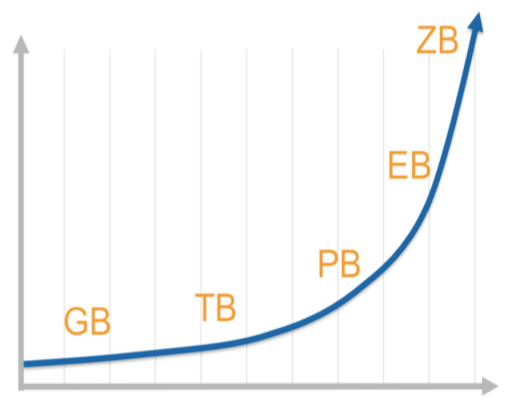
\includegraphics[width=0.5\textwidth]{images/Expgrowth.png}
    \caption{The exponential growth of data from gigabytes to zettabytes [Amazon].}
  \label{datagrowth.png}
\end{figure}
What has changed in the past few decades is the exponential rise in
available computing power, and as a related consequence, the enormous quantities and complexity of the observed data, primarily in digital form. Such data are referred to as $\textit{big data}$ and traditional data-processing tools are inadequate to deal with them. Big data are now creating, in addition to the natural world, a digital world, in which extracting new and useful information from the data already taken and archived is becoming a major endeavor in itself. This action of knowledge discovery in databases is most commonly referred to by the phrase data mining \citep{ball2010data}. The analogy is that a large volume of earth and raw material is extracted from a mine, which when processed leads to a small
amount of very precious material; similarly, in data mining, a large volume
of data is processed to construct a simple model with valuable use, for example, having high predictive accuracy \citep{alpaydin2014introduction}.



\section{An Introduction to machine learning}
\label{Intro}

To solve a problem on a computer, we need an algorithm. An algorithm
is a sequence of instructions that should be carried out to transform
the input to output. For example, one can design an algorithm for
sorting, where the input is a set of numbers and the output is an ordered
list. For the same task, there may be various algorithms and one may be
interested in finding the most efficient one, requiring the lowest number of
instructions or memory. For some tasks, however, one does not have an algorithm, for example to tell spam email from legitimate email. Therefore what we lack in knowledge, we make up for in data. One can easily compile thousands of example messages, some of which one knows to be spam and what one wants is to "learn" what constitutes spam \citep{alpaydin2014introduction}. 

Learning is what gives us flexibility
in our lives, the fact that we can adjust and adapt to new circumstances, and learn new
tricks, no matter how old we are. The important parts of human or animal learning are remembering, adapting and generalising. Being able to recognize late events, and to know which actions are to be taken, and also knowing how to distinguish between different situations, so that things that applied in one place can be used in another, is what makes learning useful \citep{marsland2015machine}. 

 Machine learning is not only a database problem, but is also part
of artificial intelligence. For a system to be intelligent, it needs to have the ability to learn and adapt in a changing environment. If the system can learn and
adapt to changes, then it can easily predict future solutions not provided by the system designer \citep{alpaydin2014introduction}. This involves tasks such as recognition, diagnosis,
planning, robot control, prediction, etc \citep{nilsson1996introduction}.
Machine learning also helps one find solutions to many problems in vision,
speech recognition, and robotics. Machine learning is programming computers to optimize a performance criterion using example data or past experience. One has a model defined
up to some parameters, and learning is the execution of a computer program
to optimize the parameters of the model using the training data or
past experience. The model may be predictive to make predictions in the
future, or descriptive to gain knowledge from data.
Machine learning uses the theory of statistics in building mathematical
models, because the core task is making inference from a sample \citep{alpaydin2014introduction}.


Given a class of tasks T, an experience E and measure of performance P, a computer program is said to learn from E with respect to T if the measure P at T improves for more observations E provided \citep{michalski2013machine}. 
\subsection{Examples of machine learning}
We are surrounded by machine learning-based technology such as online shopping where  search engines learn how to bring us the best results and a list of the most relevant products related to our search, email (spam filters, smart email categorization, etc)  where anti-spam software
learns to filter our email messages into spam or not-spam using simple rule filters. A similar approach is used by Gmail to categorize our emails into primary, social, and promotion inboxes, as well as labelling emails as important. 

In a research paper, "The Learning Behind Gmail Priority Inbox" \citep{aberdeen2010learning}, Google outlines its machine learning approach  and notes: " When a user marks messages in a consistent direction, we perform a real-time increment to their threshold." Every time the user marks an email as important, Gmail learns. The researchers tested the effectiveness of Priority Inbox on Google employees and found that those with Priority Inbox "spent 6\% less time reading email overall, and 13\% less time reading unimportant email.", social networking (Facebook, etc) Facebook  automatically highlights faces and suggests friends to tag when uploading a photo. A similar approach is used on digital cameras to learn how to detect faces,  mobile use (voice-to-text, smart personal assistants)  where smartphones today are equipped with a standard feature to convert voice to text; by pressing a button or saying a particular phrase ("OK Google", for example), you can start speaking and your phone converts the audio into text and recognizes voice commands \citep{Techemergence}.  
Machine learning is also widely used in scientific applications such as bioinformatics, medicine, and astronomy.


One common feature of all of these applications is that, in contrast to more
traditional uses of computers, in these cases, owing to the complexity of the patterns that need to be detected, a human programmer cannot provide an explicit, finely detailed specification of how such tasks should be executed \citep{shalev2014understanding}, since in recent years, the world's technology has become increased consistently, as shown in Figure \ref
{datagrowth.png}. This escalation led to the amount of data available for learning increasing dramatically. We therefore provide several reasons why machine learning is important, given the data challenges.
\begin{itemize}

\item Machine learning methods can often be used to extract the important relationships and correlations of hidden information among "big data". This is also referred to as data mining.

\item The amount of information available about certain tasks might be too large for humans to encode, whereas machines can learn this knowledge gradually and be able to capture more of it than humans would \citep{nilsson1996introduction}.

\item Some tasks cannot be defined well except by example; that is, we might be
able to specify input or output pairs but not a concise relationship between
inputs and desired outputs. We would like machines to be able to adjust
their internal structure to produce correct outputs for a large number of
sample inputs and thus suitably constrain their input or output function to
approximate the relationship implicit in the examples \citep{nilsson1996introduction}.
\end{itemize} 

Our focus will be based mainly on tasks that are beyond human capabilities. These are families of tasks that are related to the analysis of very large and complex data sets such as astronomical data. With more and more available digitally recorded data, it becomes obvious that there are treasures of meaningful information buried in data archives that are much too large and too complex for humans
to make sense of. Learning to detect meaningful patterns in large
and complex data sets is a promising domain in which the combination
of programs that learn with the almost unlimited memory
capacity and ever increasing processing speed of computers opens up new horizons \citep{shalev2014understanding}.

\subsection{Types of machine learning}

\begin{figure}[H]
  \centering
    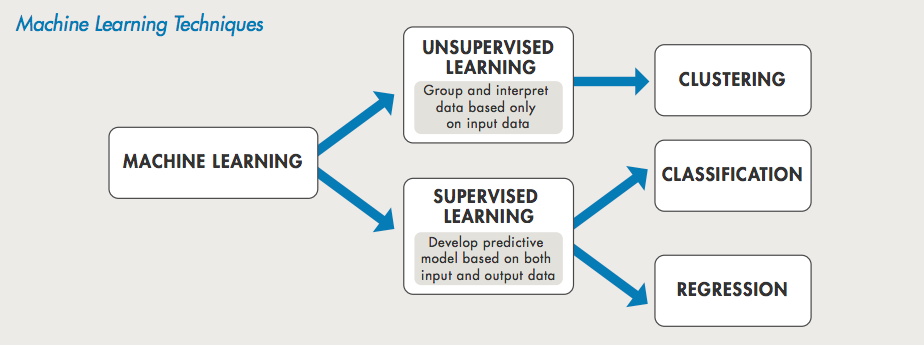
\includegraphics[width=0.7\textwidth]{images/Ml_techs.png}
    \caption{Machine learning techniques include both supervised and unsupervised learning \citep{Machinelearning}.}
  \label{sup-unsup}
\end{figure}

Machine learning algorithms are broadly divided into supervised and unsupervised methods, also known as predictive and descriptive, respectively. In supervised learning, the goal is to predict the value of an outcome measure based on a number of input measures, as one has an idea about the relationship between the input and output based on the training data set. In contrast to supervised learning, unsupervised learning occurs in the sense that the data can speak for themselves
without preconceptions such as expected classes being imposed \citep{ball2010data}. 

\subsubsection{Supervised learning}
The aim of supervised machine learning is to build a model
that makes predictions based on evidence in the presence of
uncertainty. Suppose  one wants want to fit a model $\textbf{Y}=f(\textbf{X})+\epsilon$ with errors $\epsilon$ being additive. Supervised learning attempts to learn the function $f$ by examples given through a teacher, given the training set with input and output observations $T=(x_i,y_i ), i=1,\dots N$. The observed input values $x_i$ are fed into an artificial system, known as a learning algorithm, which produces outputs $\widehat{f}(x_i)$ in response to the inputs. The learning algorithm has the property that it can modify its input/output relationship $\widehat{f}$ in response to the error $y_i- \widehat{f} (x_i)$ between the original and predicted outputs. This process is known as learning by example. Upon completion of the learning process the hope is that the predicted and real outputs will be close enough to be useful for all sets of inputs likely to be encountered in practice \citep{friedman2001elements}.

Supervised learning uses classification and regression techniques
to develop predictive models. Depending on the given dataset, variables can be characterized as either quantitative or qualitative (also known as categorical). Quantitative variables take on numerical values. Examples include a person's age, height, air temperature, wind speed, etc. whereas, qualitative variables take on input vectors and decide which of N classes
they belong to as shown in Figure \ref{RC}, based on training from exemplars of each class or category. Examples of qualitative variables include a person’s gender (male or female) or whether a person defaults on a debt (yes or no) \citep{aitkin2009statistical}. Qualitative variables are typically represented numerically by codes. The easiest case is when there are only two classes or categories, such as "success"
or "failure", "survived" or "died". These are often represented by a single binary digit or bit as 0 or 1, or else by -1 and 1. For reasons that will become apparent, such numeric codes are sometimes referred to as targets \citep{friedman2001elements}. In machine learning, if the label is numerical, the task is called regression and the learner is also called a fitted regression model, while if the label is categorical, the technique is called classification and the learner is also called a classifier. For both techniques, the training process is conducted on data sets containing label information or examples \citep{zhou2012ensemble}.

\begin{figure}[H]
  \centering
    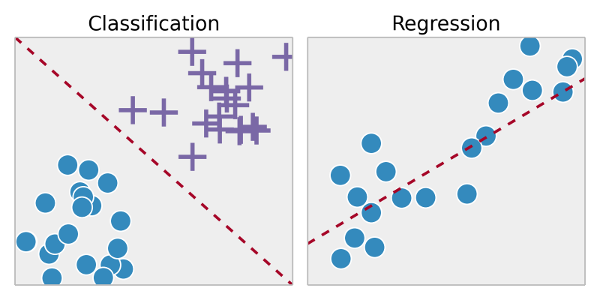
\includegraphics[width=0.7\textwidth]{images/RC.png}
    \caption{Example of classification and regression \citep{rossant2018ipython}.}
  \label{RC}
  
\end{figure}
Classification tasks are mostly known to be discrete, i.e. each example belongs to only one class, and the set of classes covers the whole possible output space; whereas regression tasks are known to be continuous \citep{stephen2009machine}. However there are some overlaps between the algorithms for these tasks. A classification algorithm may predict a continuous value, but the continuous value is in the form of a probability for a class label and a regression algorithm may predict a discrete value, but the discrete value is in the form of an integer quantity. Some algorithms can be used for both classification and regression with small modifications, such as decision trees and artificial neural networks \citep{brownlee2013prepare}.  

\subsubsection{Unsupervised learning}

In contrast to labelled data, unlabeled data (i.e., data items without associated labels) can often be obtained in great quantities without much additional effort. The unsupervised learning technique aims at making use of the (additional) information provided by the unlabelled patterns to generate appropriate models. 

As illustrated in Figure \ref{sup-unsup}, in unsupervised learning one has only a set observations $T=x_1,x_2,\dots, x_N$. In unsupervised learning one is not interested in prediction, because one does not have an associated output response variable $y_1,y_2,\dots, y_N$. Rather the goal in unsupervised learning algorithms is to discover interesting information about the measurements on the training set $T$. one looks for an informative way to visualize the data and interesting patterns among the observations \citep{james2013introduction}. 

\begin{figure}[H]
  \centering
    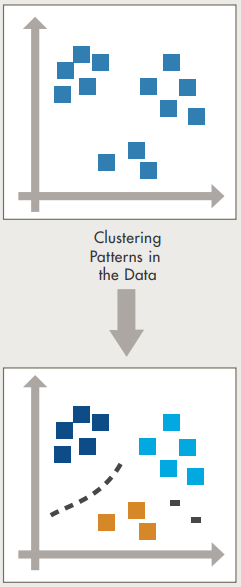
\includegraphics[width=0.35\textwidth]{images/cluster.png}
    \caption{An example of clustering method which reveals hidden patterns in data \citep{Machinelearning}.}
  \label{datagrowth.png}
\end{figure}

Clustering is one of the most commonly used unsupervised methods that divide data into clusters. The number of clusters must initially be specified, but since the algorithm converges rapidly, many starting points can be tested. The algorithm uses a distance
criterion for cluster membership, such as the Euclidean distance, and a stopping criterion for iteration, for example, when the cluster membership ceases to change \citep{ball2010data}.

\section{Process of machine learning}
\label{Process}
\subsection{Data preparation}
Machine learning algorithms learn from data, therefore it is critical that one feed them the right data for the specific problem one want to solve. In this section we will describe the processing steps required for getting data ready for a machine learning algorithm.

Three steps commonly used in machine learning to process the data, namely data selection, data preprocessing  and data transformation. Data selection has to do with the selection of the the subsets of all available data that one need to address the question or problem on which we are working. Usually assumptions will be made  about the data and be tested at a later stage. After selecting the data, comes the preprocessing step where one decide how to use the data. Firstly, suitable formatting of the data is considered, which could be .csv file format or Numpy file format. In most cases there may be data instances that are incomplete or do not contain useful information. Such cases, the removal or fixing of such data is required. When generating the training dataset, it is crucial  also consider the computational cost and memory requirement. Sampling the data by taking a smaller representative sample of the selected data may be much faster for exploring and prototyping solutions before considering the whole dataset. The final step is to transform data using scaling, where the preprocessed data may contain attributes with a mixture of scales for various quantities and are scaled to range between 0 and 1. This helps to stop the weights from getting too large unnecessarily \citep{marsland2015machine}. One could also use decompositions, which involve attributes that represent a complex concept that may be more useful to a machine learning method when split into the constituent parts, and  aggregations where attributes can be aggregated into a single attribute that would be more meaningful to the problem being solved \citep{brownlee2013prepare}. The most commonly used scaling methods are referred to as data normalisation, or standardisation \citep{marsland2015machine}.
    
\subsection{Feature engineering}

In machine learning applications, whether classification or regression, observation
data that one believes contain information are taken as inputs and fed
to the system for decision-making. Some of the goals in these learning algorithms are to achieve the following objectives: improving the prediction performance of the model and reducing the model complexity. This could help reduce the estimation error and thus prevent overfitting. If one assumes that the observation data $\textbf{X}=\mathbb{R}^d$ \citep{shalev2014understanding}, then in most learning algorithms, the complexity depends on the number of
input dimensions, $d$, as well as on the size of the data sample, $N$. 
For reduced memory and computation, one is interested in reducing
the dimensionality of the problem such that one has a new feature space $\mathbb{R}^k$ of dimension $k \ll d $. Decreasing $d$ will also decreases the
complexity of the inference algorithm during testing. The
complexity is often broken into two parts: the complexity of training, and the complexity of applying the trained algorithm. Training does not happen very often, and is not usually time-critical. However, we often want a decision about a test point quickly, and there are potentially many test points when an algorithm is in use, so this needs to have low computational cost \citep{marsland2015machine}.

When data can be explained with fewer features, one gets a better idea about the process that underlies the data and this allows knowledge extraction. There are two main methods for reducing dimensionality: feature selection and feature extraction. In feature selection, one is interested in
finding $k$ of the $d$ dimensions that give the most information such that the other $(d - k)$ dimensions is discarded. In feature extraction, one is interested in finding a new set of $k$ dimensions that are combinations of the original d dimensions \citep{alpaydin2014introduction}.
 
During algorithm learning, a feature $x_i\in\mathbb{R}$ becomes relevant to a target concept $t$ (what is being learned) if  a pair of examples A and B in the instance space such that A and B exists differ only in their assignment to  $x_i$ \citep{blum1997selection}. This implies that adjusting the value of $x_i$ affects the desired output of the learning algorithm. Hence it is important to identify the features that are most useful for the problem under examination. This invariably requires prior knowledge of the problem and the data. This process is called feature selection.

In any machine learning, algorithm technique selection is mostly driven by the structure of the dataset and type of problem one wishes to solve (regression or classification). Therefore it is important to have better understanding of the dataset and which features are useful prior to the selection and splitting of the dataset, as described in the previous paragraph. The output of the problem is real number, one therefore categorize the problem as regression. The identified algorithms that are applicable and practical to implement are multi-output regression algorithms to be discussed in more details in the next chapter. 


\section{Tuning model complexity}
\label{comp}
In prediction models, prediction errors can be decomposed into error due to bias and error due to variance. There is a tradeoff between a model's ability to minimize bias and variance during training \citep{fortmann2012understanding}. 
\subsection{Bias and variance }
Understanding these two types of error can help us diagnose model results and avoid the mistake of over- and underfitting. Understanding the bias and variance will help one to improve the data fitting process, resulting in more accurate models \citep{fortmann2012understanding}.
Error due to bias is the difference between the average prediction of  models and the true value which one is trying to predict. For example, assuming one has multi-models built from a dataset generated randomly, this will result in the models yielding multi-predictions, hence the bias measures how far off in general these model's predictions are from the true value. Error due to variance is the variability of a model prediction for a given data point \citep{fortmann2012understanding}. 

\begin{figure}[H]
  \centering
    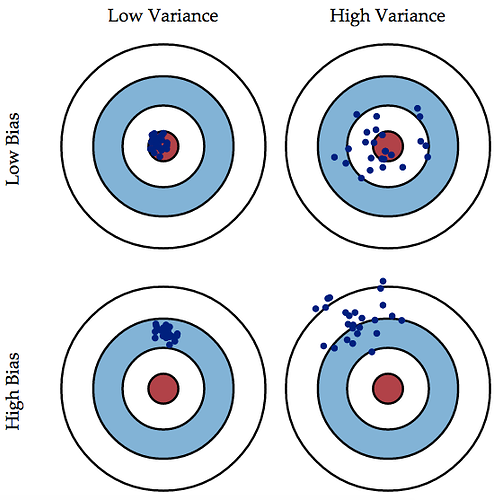
\includegraphics[width=0.48\textwidth]{images/Bias.png}
    \caption{Graphical illustration of bias and variance. The center of each target represents a model that perfectly predicts the true value and as one moves away from the centre, the model gets worse at predicting the true value. Variability in the training dataset due to outliers or non-standard values will also result in poor prediction \citep{fortmann2012understanding}.}
  \label{RC}
 \end{figure}
 
Suppose  one has a training set $\textbf{X}=\{x_1,\dots x_n\}$ and and a function $\textbf{Y}=f(\textbf{X})+\epsilon$ with $\epsilon$ being an error term normally distributed with zero mean and variance $\sigma^2$. One wants to find a function $\widehat{f}(\textbf{X})$  that estimates $f(\textbf{X})$ as well as possible using some learning algorithm technique. In this case, one measures the mean squared prediction error at a point $x$ as :
\begin{align*}
Err(x)&= \mathbb{E}\left[(\textbf{Y}- \widehat{f}(x) ) \right]\\
&= \mathbb{E}\left[ \textbf{Y}^2 +\widehat{f}(\textbf{x})^2 -2\textbf{Y}\widehat{f}(x)\right]\\
&= \mathbb{E}\left[\textbf{Y}^2 \right] + \mathbb{E}\left[\widehat{f}(x)^2 \right]- 2\mathbb{E}\left[\textbf{Y}\widehat{f}(x)\right]
\end{align*}
Since $\text{Var}(\textbf{Y}) = \mathbb{E}\left[\textbf{Y}^2 \right]- \mathbb{E}\left[\textbf{Y}\right]^2$, then we have  $\mathbb{E}\left[\textbf{Y}^2 \right] =\text{Var}(\textbf{Y}) + \mathbb{E}\left[\textbf{Y}\right]^2$, such that
\begin{align*}
Err(x)&= \text{Var}(\textbf{Y}) + \mathbb{E}\left[\textbf{Y}\right]^2 + \text{Var}\left[\widehat{f}(x)\right] + \mathbb{E}\left[\widehat{f}(x) \right]^2- 2f\mathbb{E}\left[\widehat{f}(x) \right]\\
&= \text{Var}(\textbf{Y}) + \text{Var}(\widehat{f}) + (f(x)- \mathbb{E}\left[
\widehat{f}\right]^2)\\
&= \sigma^2 + \text{Var}(\widehat{f})+ \text{Bias}\left[\widehat{f}\right]^2
\end{align*}

where $\sigma^2$ represents the irreducible error. 

There are various ways of managing the bias and variance during training, one of them being bagging and resampling. These techniques can be used to reduce the variance in model prediction. In bagging (bootstrap aggregating), replicates of the original data set are created using random selection with replacement. Each randomly selected data set is then used to construct a new model and the models are gathered together into an ensemble. To make a prediction, all the models in the ensemble are polled and their results are averaged.

\subsection{Overfitting and underfitting}

\begin{figure}[H]
  \centering
    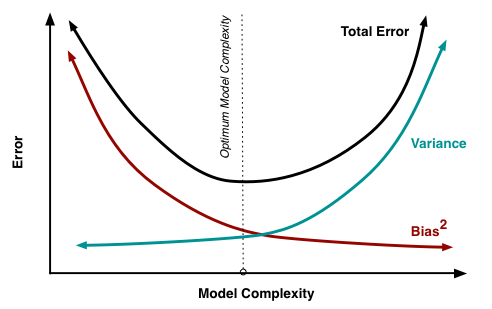
\includegraphics[width=0.7\textwidth]{images/biasvariance.png}
    \caption{The bias and variance contributing to total error. Dealing with bias and variance is about dealing with overfitting and underfitting. The bias is reduced and the variance is increased in relation to the model complexity. As more parameters are added to a model, the complexity of the model increases and variance becomes the primary concern while bias steadily decreases \citep{fortmann2012understanding}.}  
\end{figure}

Understanding bias and variance is critical for understanding the behaviour of prediction models, but in general what one really cares about is the overall error, not the specific decomposition. The optimum point for any model is the level of complexity at which the increase in bias is equivalent to the reduction in variance. If model complexity exceeds this optimum point; we are in effect overfitting our model; while if our complexity falls short of the optimum point, we are underfitting the model \citep{fortmann2012understanding}.









 % Chapters might go from 2. problem statement, 
                 % through 3. model, to 4. analysis & results
\chapter{ZCal - calibrating radio interferometric data with machine learning}
\label{c3}
ZCal, in full "Zitha calibration" is a new machine learning radio data calibration experiment through which one make use of the telescope sensor data to determine the relationship with calibrator solutions obtained using conventional calibration techniques. In Section \ref{Exp}, we further discuss the external parameters affecting the observed radio interferometric data, followed by a brief description of the KAT-7 telescope and  Section \ref{kat7} describes how the sensor data and calibration solutions are processed for training. In Section \ref{algo1} we define and describe the regression algorithms used for our experiment, and in Section \ref{TT} we describe the training and testing procedure of the algorithms leading to the output results of our experiment in Section \ref{sec3}. 
\section{External parameters affecting the data}
\label{Exp}
%%Each antenna in an array has a primary beam which is used for perfect resolution during an observation of a source. The resolution of each antenna is defined as =1.22 / D, where  ~ 21 cm is the  wavelength, D is the diameter of your dish and is the resolution angle. In an interferometric array of N antennas with baselines b, the resolution angle is defined as  =1.22  / d, where d is the maximum baseline in an array.   The beam of all the baselines is call a synthesised beam which is a multiplication of all the primary beams.

Astronomical observations done with interferometric radio
telescopes suffer from variable gain effects that can
broadly be classified as direction-independent and direction-dependent errors. The complex instrumental gains due to the electronic devices that follow the feed elements are directionally independent \citep{bhatnagar2008correcting}; relative amplitude and phase gain for each antenna; phase and amplitude drifts in the electronics of each antenna; amplitude response as a function of elevation (gain curve) and tropospheric amplitude and phase effects.

As defined in Chapter 1, \textit{calibration} is the process of correcting for the signal corrupted by various mechanisms. Some of these mechanisms include external parameters such as fluctuations in air temperature, weather conditions on site and antenna pointing errors \citep{taylor1999synthesis}. Antenna pointing error is the difference between the actual pointing position and the requested (to go) position. Though an array consists of more than one antenna, each with a tracking centre, during a request ("POINT"), they must all follow the same required position. However, this is not always accurate, owing to misalignment of the elevation axis, atmospheric refraction, gravitational deformation of the structure, differential heating of the structure and wind loading \citep{taylor1999synthesis}. Wind loading is an effect that degrades the pointing accuracy, thus the design of the telescope structure plays a role in terms of wind loads \citep{smithdynamic}. Telescopes with a large dish structure are subjected to large wind loads. The wind speed and the geometric dimensions are the cause of highly turbulent flows around the antenna. There are violent shifts in airflow on the surface and around the antenna \citep{upnere2012characterization}. The following equation \ref{sens} shows the nominal expected sensitivity of the telescope without any errors:
\begin{align}
\left[\frac{2kT_{sys}}{A_{eff}\sqrt{N(N-1)\tau \Delta \nu}}\right]
\label{sens},
\end{align}
 where ($N$ is the number of antennas in the array,  $A_{eff}$ is aperture efficiency, $\tau$ is the integration time, $k=1.38\times 10^{-23}Jk^{-1}$ is the Boltzmann constant, $\Delta \nu$ is the bandwidth and $T_{sys}=\sum T_{i}$ an additive of noise contribution from different source such as atmosphere, ground, telescope surface and receivers) \citep{wilson2013tools}. This can also introduce distortion on sources that are resolved, i.e., objects that consist of a non point-like structure as opposed to the point sources in Figure \ref{pks1613} \citep{Calibration}. 



\section{KAT-7 telescope}
\label{kat7}

\begin{figure}[H]
  \centering
    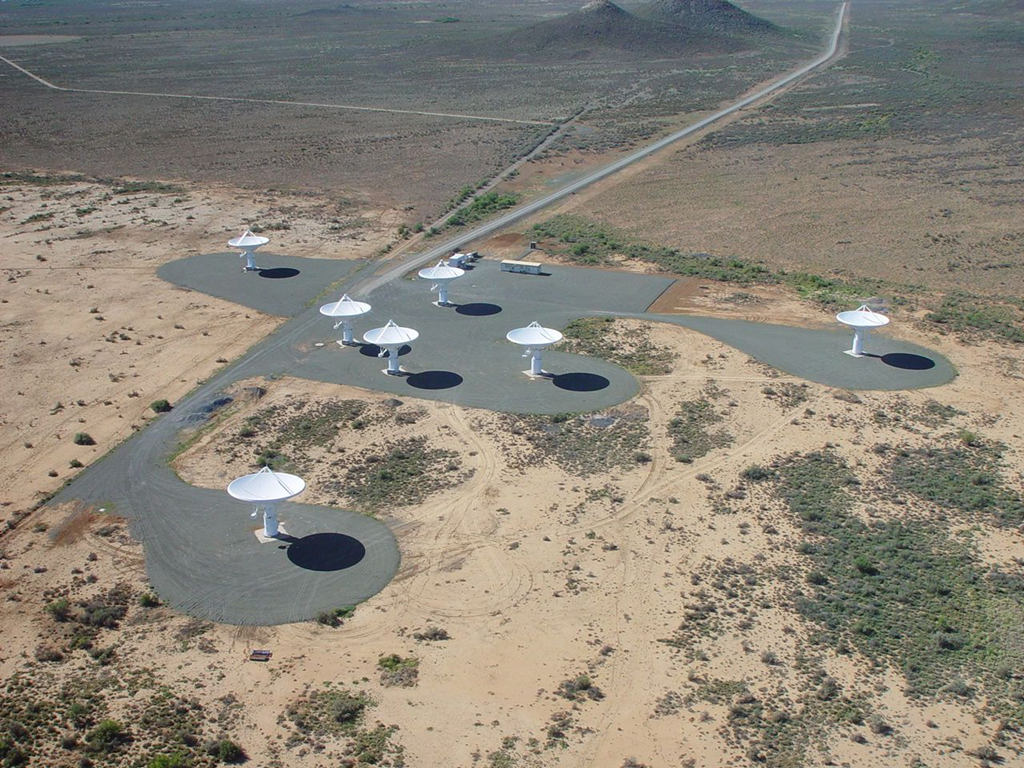
\includegraphics[width=0.6\textwidth]{images/K7.png}
    \caption{The seven-dish MeerKAT precursor array, \citep{carignan2013kat}}
  \label{images/kat7.png}
\end{figure}

The KAT-7 is a seven-dish interferometry that was built as an engineering prototype for technologies and techniques in preparation for the 64-dish Karoo Array Telescope (MeerKAT). These instruments are located in the Northern Cape Karoo desert region and are operated remotely from CapeTown. The construction of  KAT-7 began in
2008 with the writing of the telescope requirements specification and was completed in 2010.  It was operated in engineering mode until 2015  and became fully operational in 2016  \citep{foley2016engineering}. As seen in Table \ref{images/kat7.png}, KAT-7 antennas are extremely close together with baseline ranging between 26 and 185 m \citep{carignan2013kat}. More parameter specifications are presented in the Tables \ref{DSpec} and \ref{DSpec}:
\begin{table}[H]\centering
\begin{tabular}{l l }
\toprule
\textbf{Parameter} & \textbf{Value}\\
\midrule
Dish diameter&12 m \\
Number of antennas& 7\\
Min baseline & 26 m\\
Max baseline & 185 m\\
Frequency range & 1200-1950 MHz\\
Max instantaneous bandwidth &256 MHz\\
Polarization   & Linear H $\&$ V\\
Systems temperature ($T_{sys}$) & $<$35 K across the entire frequency band\\
Aperture effeciency & 0.65\\
Location &  latitude 30.7148$^{\circ}$ S, longitude 21.388 $^{\circ}$ E\\
cryogenic temperature on receiver & 80 K\\
Digital back end & Roach \\
Elevation & 1054 m\\
\bottomrule
\end{tabular}
\caption{The instrument consist of 7 12-m dishes with linearly polarized feeds. The operational lower noise amplifier for each dish is $80\;K$  with system temperature $<35\;K$. The frequency range of this instrument is $1200-1950 \text{MHz}$ with bandwidth of $256\;\text{MHz}$ \citep{foley2016engineering}.}
\label{K7 spec}
\end{table}

%\begin{table}[H]\centering
%\begin{tabular}{l l l l}
%\toprule
%\textbf{Mode}& \textbf{Total BW(MHz)} & \textbf{Number of chan} & \textbf{Chan width(KHz)} \\
%\midrule
%c16n2M4k  &  1.5625	& 4096& 	0.381\\
%c16n7M4k & 6.25 & 	4096& 	1.526\\
%c16n25M4k& 	25&	4096& 	6.104\\
%c16n400M4k&  256& 	1024& 	390.625\\
%\bottomrule
%\end{tabular}
%\caption{The table is showing different correlator modes for observations. The correlator is based
%on the so-called 'FX, architecture, i.e (Fourier transform 'F' followed
%by Cross-correlation 'X'). The F  which channelise the incoming data streams
%into spectral components and the X does the multiplication and accumulation of each and every product pair \citep{foley2016engineering}.}
%\label{K7 modes}
%\end{table}
\begin{table}[H]\centering
\begin{tabular}{l l }
\toprule
\textbf{Parameter} & \textbf{Value}\\
\midrule
Pointing accuracy & 25 $^{\prime \prime}$ \\
Wind (Operational) & 36 km/h\\
Wind (Marginal Operation) km/h & 45 km/h\\
Wind (Drive to Stow) & 55 km/h\\
Wind (Survival) & 160 km/h\\
Azimuth Rotation slew speed &  2$^\circ$/s\\
Azimuth limits & -175$^{\circ}$, +285 $^{\circ}$\\
Elevation slew speed & 1$^{\circ}$/s\\
Elevation limits & 0$^{\circ}$, 90 $^{\circ}$\\
Feed/Cryo & Mass 75 kg\\
\bottomrule
\end{tabular}
\caption{The table shows the KAT-7 dish specification \citep{foley2016engineering}.}
\label{DSpec}
\end{table}

\subsection{Sensor data}

During scientific observations, data indexed by time are continuously collected from instruments and  environment (atmospheric pressure, air temperature,  wind conditions, and relative humidity, wind direction, etc). Samples as a function of time are recorded from software and sensors attached to the telescopes with their adjoining instrumentation \citep{slabberICALEPCS2017}. Sampling strategies are set on sensors processed by the control and monitoring (CAM) system, ranging from several updates per second to infrequent updates. The typical sample in KAT-7 CAM contains the following attributes: a sensor name, sample timestamp, value timestamp, status and a value as shown in the following example, where red represents the sensor sample and green is the sensor sample description  \citep{slabber2015overview, slabber2015illustrate}. 

\definecolor{keywords}{RGB}{255,0,90}
\definecolor{comments}{RGB}{0,0,113}
\definecolor{red}{RGB}{160,0,0}
\definecolor{green}{RGB}{0,150,0}
 
\lstset{language=Python, 
        basicstyle=\ttfamily\small, 
        keywordstyle=\color{keywords},
        commentstyle=\color{comments},
        stringstyle=\color{red},
        showstringspaces=false,
        identifierstyle=\color{green}}

\begin{tcolorbox} 
\begin{lstlisting}

   {"name": wx_station_wind_speed,
   "time": 1506430493.4778199196,
   "status": nominal,
   "value_ts": 1506430493.4774999619,
   "value": 10.3}

   #SENSOR_NAME A normalised form of a sensor name.

   #SAMPLE_TS The UNIX timestamp of when the sample was
   #first processed by the CAM system.

   #VALUE_TS A UNIX timestamp when the acquisition
   #was performed. 

   #STATUS indicate the state of the sensor when
   #the sample was taken. Can have a value of UNKNOWN,
   #WARN, NOMINAL, FAILURE, INACTIVE, ERROR, UNREACHABLE. 
\end{lstlisting}
\end{tcolorbox}

All components are interfaced to the CAM system via the Karoo Array Telescope Communication Protocol (KATCP), i.e KATCP is responsible for internal communication between CAM components and other subsystems (science data processing, correlator beamformer, etc) \citep{slabber2015overview}. A KATCP interface exposes requests and sensors. To access the sensor information for analysis, users from different subsystems  would  connect to the CAM webserver using Python client and subscribe to sensor data of interest. 

\subsection{Preparation of training data}\label{prep}

The objective of this study is to find correlations between
calibration solutions and sensor information on the telescope.
Therefore the main dataset for the study is the time-based
sensor information of each antenna.
The process of data collection encompasses all of the steps required to obtain the desired data in digital format. Methods of data collection include acquiring and archiving new observations, querying existing databases according to the science
problem at hand, and performing as necessary any cross-matching or data combining  \citep{ball2010data}.

%In this chapter we will look at modelling the behaviour patterns of individual antennas and calibration steps based on Karoo Array Telescope (KAT-7) \ref{images/kat7.png}.

In every observation, the collected data are stored by the data capturing system in the Hierarchical Data Format (HDF5), which is a set of file formats designed to store and organize large amounts of data. The HDF5 file is built into two concepts: meta-data and observed visibilities. In meta-data one finds static information of the data set, including observer, dump rate and all the available subarrays and spectral windows in the data set selection criteria (antennas, channel frequencies, targets, scan information) and sensor data of interest as a function of time. The data observed by the radio telescope are in the  form of complex numbers referred to as visibilities, as described in Chapter 1. Each source observed contains its own visibilities as a function of time along with sensor data,  which keep a record of the telescope's activity and behaviour as these are observed.

In preparation for the training and testing dataset, we look at environmental sensors and instrumental sensors
recorded during observations with a flux calibrator and a phase calibrator source
PKS1613-586 in Figure \ref{pks1613}. This was the most frequently used phase calibrator during the KAT-7 commissioning phase. A series of observations for different tests with this calibrator \ref{pks1613} were taken in the period from December 2011 to November 2014. These tests includes Circinus X-1 monitoring at frequency $2022 - 1622.391 \;\text{MHz}$; OH maser monitoring at frequency $1666.481 - 1664.919 \;\text{MHz}$, $1666.381-1666.819\;\text{MHz}$,  $1666.281- 1664.719\;\text{MHz}$; spectral dynamic range test at frequency $1669.125 - 1662.877 \;\text{MHz}$, $1678.500 - 1653.506 \;\text{MHz}$; Circinus X-1 H absorption at frequency $1425.125 - 1418.827\; \text{MHz}$, $1424.125 - 1417.877 \;\text{MHz}$ and imaging new calibrators at frequency $2022 - 1622.391 \;\text{MHz}$. The chosen sensors of interest from each observation are: 
\begin{enumerate}

\item Air temperature
\item Wind speed
\item Wind direction 
\item Air pressure 
\item Relative humidity 
\item Actual refraction elevation
\item Actual refraction azimuth
\item Actual scan elevation
\item Actual scan azimuth 
\item Actual pointing elevation
\item Actual pointing azimuth. 
\end{enumerate}
The environmental sensors measure the environmental conditions on site via the weather station installed around the telescope and the instrumental sensors (pointing) record the pointing azimuth and elevation activities of a telescope. These are examples of how each environmental and instrumental sensor are represented per antenna X.

\definecolor{keywords}{RGB}{255,0,90}
\definecolor{comments}{RGB}{0,0,113}
\definecolor{red}{RGB}{160,0,0}
\definecolor{green}{RGB}{0,150,0}
 
\lstset{language=Python, 
        basicstyle=\ttfamily\small, 
        keywordstyle=\color{keywords},
        commentstyle=\color{comments},
        stringstyle=\color{red},
        showstringspaces=false,
        identifierstyle=\color{green}}
        
        
\begin{tcolorbox}
\begin{lstlisting}
   {"name": anc_air_pressure,
   "time": 1506430493.4778199196,
   "status": nominal,
   "value_ts": 1506430493.4774999619,
   "value": 981.65}
   
   {"name": anc_gust_wind_speed,
   "time": 1506430493.4778199196,
   "status": nominal,
   "value_ts": 1506430493.4774999619,
   "value": 3.96}

   {"name": "anc_air_temperature",
   "time": 1506430493.4778199196,
   "status": "nominal",
   "value_ts": 1506430493.4774999619,
   "value": 23.96}

   {"name": anc_air_relative_humidity,
   "time": 1506430493.4778199196,
   "status": nominal,
   "value_ts": 1506430493.4774999619,
   "value": 25.87}

   {"name": anc_wind-direction,
   "time": 1506430493.4778199196,
   "status": nominal,
   "value_ts": 1506430493.4774999619,
   "value": 46.61}
\end{lstlisting}
\end{tcolorbox}

\begin{tcolorbox}
\begin{lstlisting}
   {"name": antX_pos.actual-pointm-elev,
   "time": 1506430493.4778199196,
   "status": nominal,
   "value_ts": 1506430493.4774999619,
   "value": 89.97}
   
   {"name": antX_pos.actual-pointm-azim,
   "time": 1506430493.4778199196,
   "status": nominal,
   "value_ts": 1506430493.4774999619,
   "value": -78.81}
   
   {"name": antX_pos.actual-refrac-elev,
   "time": 1506430493.4778199196,
   "status": nominal,
   "value_ts": 1506430493.4774999619,
   "value": 89.80}
   
   {"name": antX_pos.actual-refrac-azim,
   "time": 1506430493.4778199196,
   "status": nominal,
   "value_ts": 1506430493.4774999619,
   "value": -70.15}
   
   {"name": antX_pos.actual-scan-elev,
   "time": 1506430493.4778199196,
   "status": nominal,
   "value_ts": 1506430493.4774999619,
   "value": 89.82}
   
   {"name": antX_pos.actual-scan-azim,
   "time": 1506430493.4778199196,
   "status": nominal,
   "value_ts": 1506430493.4774999619,
   "value": 78.94}
   
\end{lstlisting}
\end{tcolorbox}

We access this data from the HDF5 file using the KAT-7 data access library called katdal \citep{skatelescope}. We select the sensor data of interest with time index during the telescope tracking of the flux calibrator and phase calibrator PKS1613-586. The following is a Python code example showing how the sensor time index is selected from the observations for a specific calibrator.

\begin{tcolorbox}
\begin{lstlisting}
#importing data access library
import katdal
import numpy
import time

#Opening the observation file 
hdf5=katdal.open('1329697773.h5')
#Selecting data of interest from the the observation file
hdf5.select(scans='track',
            targets=['PKS1934-63','PKS1613-586'],
            channels=slice(199,800)
            )   
#Obtaining sensor timestamps            
h5df5_timestamps=[]
temp_time = np.empty((len(h5.timestamps)))
for i in range(0,len(h5.timestamps)):
    temp_time[i]=(h5.timestamps[i])
    timeh5.append(T.ctime(temp_time[i]))      
       
#Selecting time during the scan of the calibrators
Time_Scan=[]
for scan in hdf5.scans() :
    #Taking average of start and endtime scan of calibrator source
    Average=((hdf5.timestamps[0]+
              hdf5.timestamps[len(hdf5.timestamps)-1])/2
             ) 
    Time_Scan.append(time.ctime(Average))
    
#obtaining time index of telescope sensors and scan time.
Time_index=numpy.where(np.in1d(numpy.unique(h5df5_timestamps),
                       Time_Scan))[0]
                       
                                           
\end{lstlisting}
\end{tcolorbox}

 The katdal library can manipulate the HDF5 observation file in many ways, including file format conversion from HDF5 to measurement sets (MS). This option is useful for astronomers using CASA for data calibration and visualization \citep{foley2016engineering}. This conversion also provides an option whereby one flags all channels affected with known radio frequency interference (RFI). Once the observation file has been converted to ms format, hand flagging for unknown RFI is performed inside CASA using the task $\textit{flagdata}$ for H and V cross correlation products. After satisfactory flagging of the data, one then proceeds to the calibration step. 
 
The systematic time-dependent complex gain errors denoted by $J_{ij}$ (where $i,j$ represent the baseline of two or more antennas) in the visibility data are almost always the dominant calibration effect, and a solution for them is necessary before proceeding with any other calibration \citep{ott2013casa}. In this dissertation we only focus on the 1GC calibration with an interest in obtaining complex gain calibration solutions for the phase calibrator PKS1613-586. In the process of 1GC, as explained in chapter 1, the complex gain calibration ($\textit{gaincal}$)  CASA task determines the time-based complex antenna gains solutions $G$ (amplitude and phase) for each polarization H \& V and each spectral window, from the visibility data of the specified phase calibration source PKS1613-586 and stores these in calibration tables.
 
These solutions are calculated based on reference antenna 5 in our case, since it is an antenna that is reasonably close to the center of the array and it was known to be particularly stable with no drop-outs during KAT-7 commissioning \citep{ott2013casa}. The task $\textit{gaincal}$ in CASA factors $J_{i,j}$ into antenna-based components, so one does not see a set of values for each baseline, but rather only one for each antenna ($J_i$) \citep{CosmoAIMS}. 

Since our phase calibrator PKS1613-586 have an unknown flux density, the obtained values of the antenna based amplitude solutions differ from the correct ones by a factor depending only on the true source flux density by 

\begin{equation}
\frac{1 \mathrm{Jy}}{(\text{true source flux density})^{0.5}},\;  \text{where 1Jy is the assumed flux density for \text{PKS1613-586}}.
\end{equation} 

We then used one of the following flux-density calibrators with known flux models: PKS1934-63, 3C147, 3C286 tied to the Perley-Taylor 99 to scale the correct gain amplitude of the phase calibrator in Figure \ref{pks1613} so that it matched the correctly scaled amplitude solutions for the flux-density calibrators as well as possible by running a CASA task $\textit{fluxscale}$ \citep{CosmoAIMS}. This process is called $\textit{bootstrapping}$. After obtaining the final table with correct amplitude and phase complex gain solutions for the phase calibrator in Figure \ref{pks1613}, we then used the complex solutions matrix written to the "CPARAM" column to generate the training and testing calibration solution data per antenna $i$. An example of the complex gain amplitude and phase solutions is shown in Figures \ref{amp} and \ref{phase}. These solutions were obtained using the CASA task $gaincal$ described in Chapter 1. 

The following code shows how the parameters were set in standard practice of 1GC as described in chapter 1 section \ref{caltech}.

\begin{tcolorbox}
\begin{lstlisting}
#Set flux for flux calibrator
default(setjy)
vis = msfile
field = flux_calibrator
fluxdensity  = -1
standard = 'Perley-Taylor 99'
setjy()

#Bandpass calibration
default(bandpass)
vis = msfile
caltable = bandpasstable
field = flux_calibrator
refant = reference_antenna
solnorm = True
combine = 'scan'
solint = 'inf'
bandtype = 'B'
minsnr = 5
interp = ['nearest']
bandpass()
\end{lstlisting}
\end{tcolorbox}
\begin{tcolorbox}
\begin{lstlisting}
#Calculating G solution for flux calibrator 
default(gaincal)
vis = msfile
caltable = gaintable
field = flux_calibrator
solint = 'inf'
refant = reference_antenna
gaintype = 'G'
calmode = 'ap'
solnorm = False
minsnr = 5
gaintable = [bandpasstable]
interp = ['nearest']
gaincal()
  
#G solution for gain calibrator
default(gaincal)
vis = msfile
caltable = gaintable
field = gain_calibrator
solint = 'inf'
refant = reference_antenna
gaintype = 'G'
calmode = 'ap'
append=True
solnorm = False
minsnr = 5
gaintable = [bandpasstable]
interp = ['nearest']
gaincal()   

#Scaling flux density for phase calibrator
default(fluxscale)
vis = msfile
caltable = gaintable
fluxtable = fluxtable
reference = flux_calibrator
transfer = gain_calibrator
fluxscale()
\end{lstlisting}
\end{tcolorbox}
A multi-frequency synthesis image deconvolution was carried out using the $\textit{CLEAN}$ CASA task with an image size of  $256 \times 256$ and cell size of $30$ arc seconds. The image rms noise in Figure \ref{pks1613} was measured using the rms noise of the 0 iteration residual image.
\begin{tcolorbox}
\begin{lstlisting}
     clean(vis='CircinusX-1.split.ms',
     imagename='PKS1613586.im',
     niter=10000,threshold='3.0mJy',
     psfmode='hogbom',
     interactive=False,
     imsize=512,
     cell='30arcsec',
     stokes='I',
     weighting='briggs',
     mode='mfs',
     usescratch=True)
\end{lstlisting}
\end{tcolorbox}
 \begin{figure}[H]
 \centering
    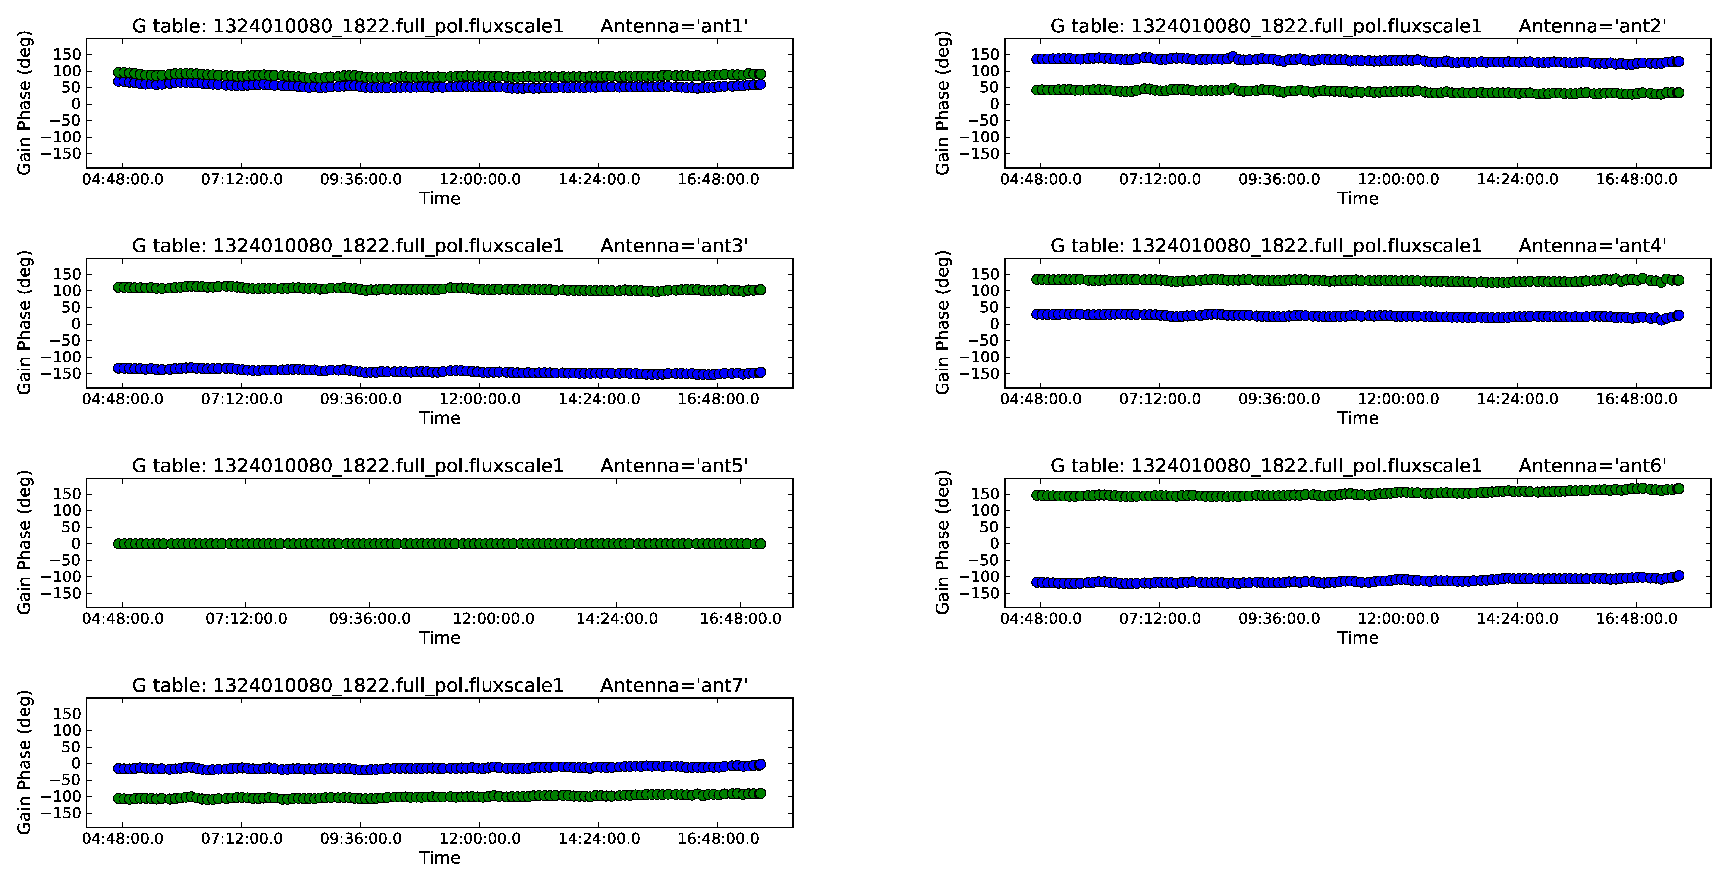
\includegraphics[ height=13cm, width=15.5cm]{images/phaseCasa.eps}
    \caption{Complex gain phase solutions for phase calibrator PKS1613-586 obtained from CASA per antenna $i$. Blue is H-polarization and green is V-polarization. Antenna 5 shows zero phase since it is used as a reference antenna.}
  \label{phase}
\end{figure}

 \begin{figure}[H]
 \centering
    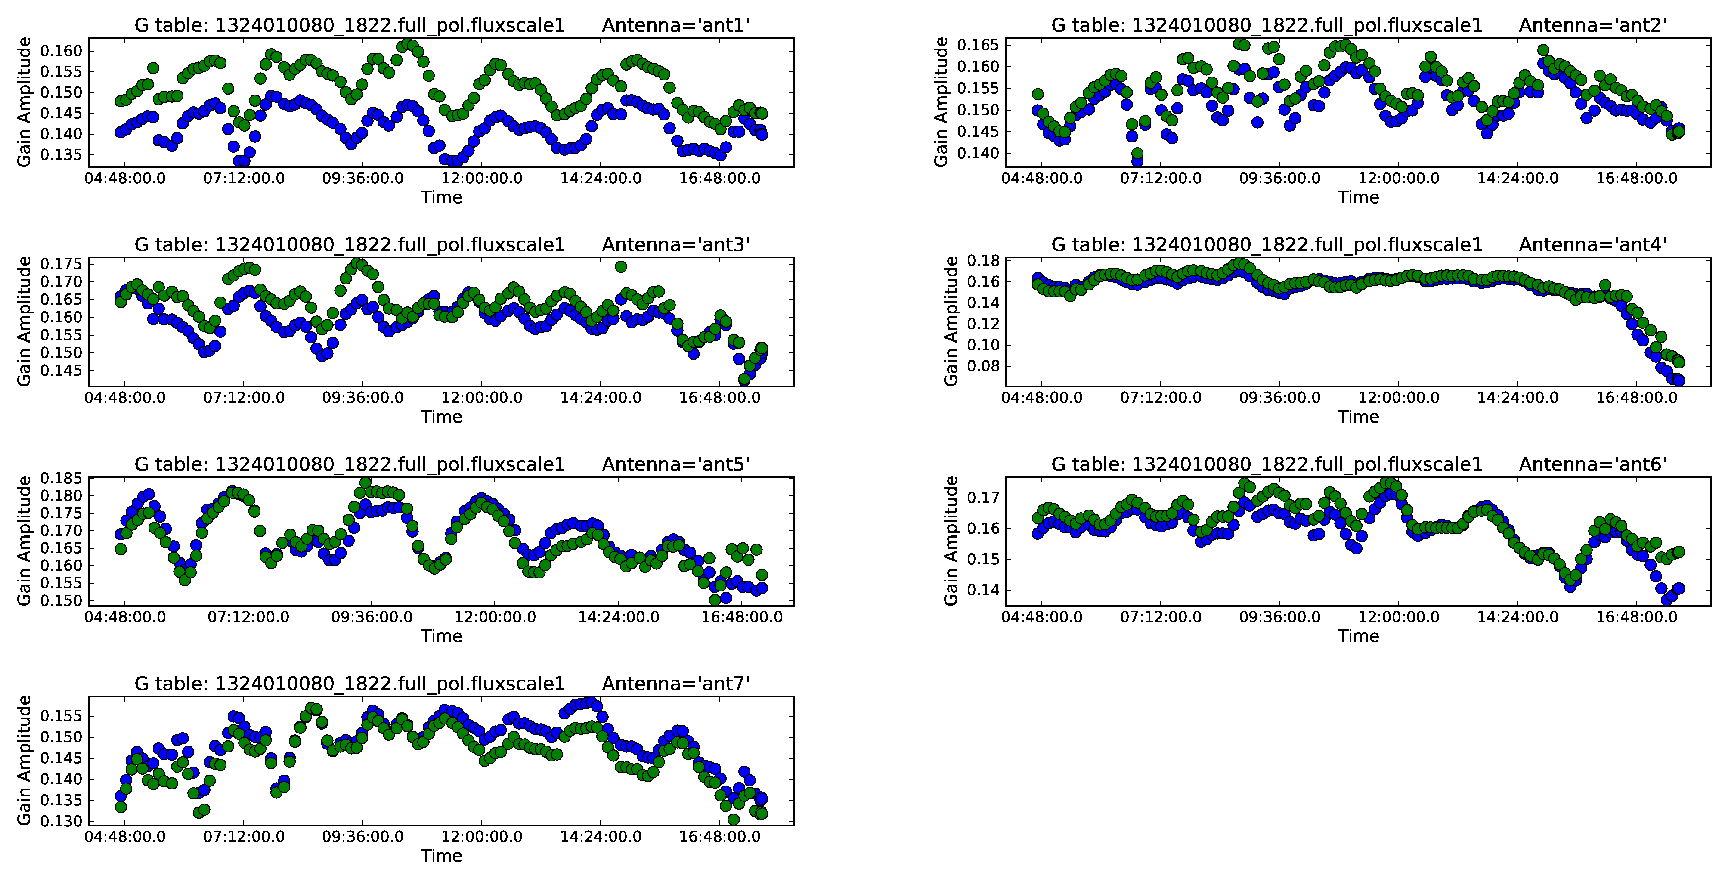
\includegraphics[ height=13cm, width=15.5cm]{images/CasaAmp.eps}
    \caption{Complex gain amplitude solutions for phase calibrator PKS1613-586 obtained from CASA per antenna $i$. Blue is H-polarization and green is V-polarization. }
  \label{amp}
\end{figure}
 
 \begin{figure}[H]
 \centering
    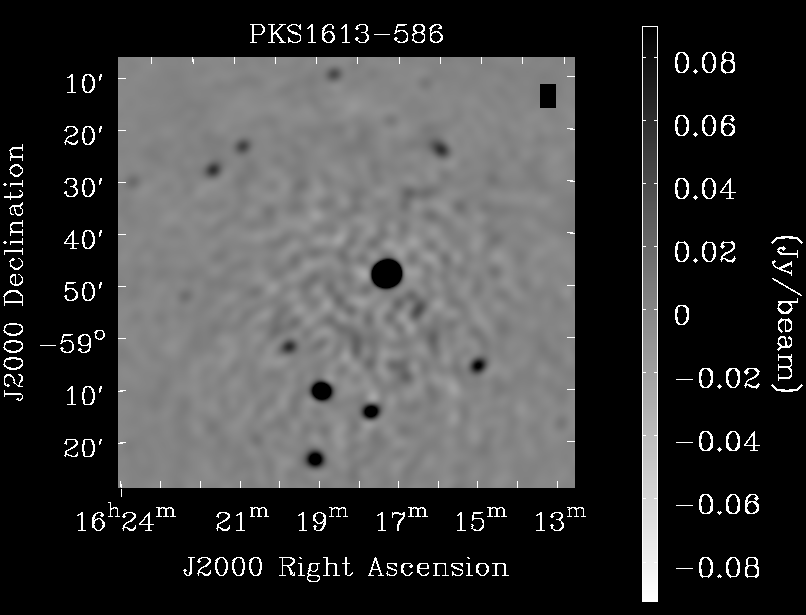
\includegraphics[ height=8cm, width=10cm]{images/162.png}
    \caption{An image of the phase calibrator PKS1613-586 located at RA, Dec (J2000): 16:17:17.88951, -58:48:07.8604. Its flux density in $Jy$ at $\text{frequency}=1.82688e^{+09} \text{Hz}$ is $4.59973 \pm 0.0146351$. This flux scaling was carried out in CASA using a strong flux calibrator. The expected rms noise of this image was calculated to be $0.08\;Jy$ using $\textit{CLEAN}$ task in CASA.}
  \label{pks1613}
\end{figure}
\section{Regression algorithm} 
\label{algo1}
Many different approaches employed in machine learning regression. These approaches learn the relationship between the input and output by fitting a model directly from the data. The fitting process involves the adjustment and optimization of hyper-parameters to minimize the prediction error. This is usually done in an independent validation and testing dataset. In this study, we consider tree-based approaches: Decision tree, random forest, extremely randomized tree and the neighbourhood search approach: (K-nearest neighbor) to tackle our problem. Firstly, we formulate our regression estimation problem as follows. Suppose we have a feature matrix 
\begin{align*}
\textbf{X}_{t}=\begin{bmatrix}
    x_{11} & x_{12} & x_{13} & \dots  & x_{1n} \\
    x_{21} & x_{22} & x_{23} & \dots  & x_{2n} \\
    \vdots & \vdots & \vdots & \ddots & \vdots \\
    x_{d1} & x_{d2} & x_{d3} & \dots  & x_{dn}
\end{bmatrix}=(x_{i,j}) \in  \mathbb{R}^{d \times n}\;, i\in \left\{1,2,\dots, d\right\}, j \in \left\{1,2,\dots,n\right\}
\end{align*}
where each column represents a vector of length d containing unique features, 
\begin{align*}
\textbf{x}_j=\begin{bmatrix}
    x_{1,j}  \\
    x_{2,j} \\
    \vdots \\
    x_{d,j} 
\end{bmatrix},
\end{align*}
with each row a vector of length n, containing the n variable measurements for the ith observation, i.e 
\begin{align*}
\textbf{x}_i=\begin{bmatrix}
    x_{i,1}  \\
    x_{i,2} \\
    \vdots \\
    x_{i,n} 
\end{bmatrix},
\end{align*}

and we also have a matrix of complex target variables to learn and predict on,
\begin{align*}
\textbf{Y}_{t}=\begin{bmatrix}
    y_{11} & y_{12} & y_{13} & \dots  & y_{1m} \\
    x_{21} & y_{22} & y_{23} & \dots  & y_{2m} \\
    \vdots & \vdots & \vdots & \ddots & \vdots \\
    y_{d1} & y_{d2} & y_{d3} & \dots  & y_{dm}
\end{bmatrix}=(y_{k,l}) \in  \mathbb{C}^{d \times m},  k\in \left\{1,2,\dots, d\right\}, l \in \left\{1,2,\dots,m\right\}
\end{align*}
where each column represents a vector of length d, containing unique target variables as a function of time $t$
\begin{align*}
\textbf{y}_{l}=\begin{bmatrix}
    y_{1,l}  \\
    y_{2,l} \\
    \vdots \\
    y_{d,l} 
\end{bmatrix},
\end{align*} 
with each row a vector of length m, containing the m variable measurements for the $kth$ observation, that is 
\begin{align*}
\textbf{y}_k=\begin{bmatrix}
    y_{k,1}  \\
    y_{k,2} \\
    \vdots \\
    y_{k,m} 
\end{bmatrix},
\end{align*}
 
The problem is to construct a learning machine, $M:\textbf{X}_{t} \rightarrow \textbf{Y}_{t}$, which when given a validation set of sensor examples, $\textbf{X}^*_{t}$, minimises some measure of discrepancy between its prediction $M(\textbf{X}^*_{t})\approx\widehat{\textbf{Y}}_{t}$, and the value of $\textbf{Y}_{t}$, where M represents the predictor. We measure the discrepancy using four commonly used statistical measures in regression \citep{borchani2015survey}: coefficient of determination, explained variance, mean squared error (MSE) and mean absolute error (MAE). The coefficient of determination is given by:

\begin{equation}
R^2\left[\textbf{Y}_{t},\widehat{\textbf{Y}}_{t}\right]=1-\frac{\sum_{k} \left[(\textbf{Y}_{t})_{k}-(\widehat{\textbf{Y}}_{t})_{k}\right]^2}{\sum_{k}\left[(\textbf{Y}_{t})_{k}-\overline{\textbf{Y}_{t}}\right]^2}, 0 \leq R^2 \leq 1,
\label{R2score}
\end{equation}
which simply measures how well the future observations are to be predicted by M, with the best score being 1 for the best performing predictor 
where,  \begin{equation}
\overline{\textbf{Y}_{t}}=\frac{1}{d_{samples}} \sum_{k} (\textbf{Y}_{t})_{k},
\end{equation} 

is the mean value of $\textbf{Y}_{t}$ draw from d samples,  
 $\sum_{k}\left[(\textbf{Y}_{t})_{k}-\overline{\textbf{Y}_{t}}\right]^2$ is the total sum of squares which measures the total variance in the predictor and $\sum_{k} \left[(\textbf{Y}_{t})_{k}-(\widehat{\textbf{Y}}_{t})_{k}\right]^2$ the residual sum of squares (deviations predicted from actual values of data), which measures the discrepancy between $\textbf{Y}_{t}$ and $\widehat{\textbf{Y}}_{t}$ \citep{james2013introduction}.

The explained variance
\begin{equation}
V=\frac{\text{Var}\left[\textbf{Y}_{t}-\widehat{\textbf{Y}}_{t} \right]}{\text{Var}\left[\textbf{Y}_{t}\right]}, 0 \leq V \leq 1, 
\label{ExV}
\end{equation}  

measures the proportion to which the predictor accounts for the variation of the observed data $\textbf{Y}_{t}$ \citep{bellinger2016fundamental}. The best possible score is considered to be 1. where 

\begin{align*}
\text{Var}\left[\textbf{Y}_{t}\right]&=\mathbb{E}\left[(\textbf{Y}_{t}-\mu)^2\right],\; \mu=\mathbb{E}\left[\textbf{Y}_{t}\right]\\
&=\mathbb{E}\left[\textbf{Y}_{t}^2-2\textbf{Y}_{t} \mu +\mu^2\right]\\
&=\mathbb{E}(\textbf{Y}_{t}^2)- 2\mathbb{E}(\textbf{Y}_{t} \mu) + \mu^2\\
&=\mathbb{E}(\textbf{Y}_{t}^2)-2 \mu^2 + \mu^2\\
&=\mathbb{E}(\textbf{Y}_{t}^2)-\mu^2,
\end{align*}
\citep{fortmann2012understanding}

MSE and MAE, which measure the average of the squared and absolute of the errors between the the observed values $\textbf{Y}_{t}$ and the predicted $\widehat{\textbf{Y}}_{t}$. For accurate prediction of the predictor, the value of MSE and MAE should converge to zero \citep{james2013introduction}. 

\begin{align}
\text{MSE}\left(\textbf{Y}_{t},\widehat{\textbf{Y}}_{t} \right)=\frac{1}{d_{samples}} \sum_{k} (\textbf{Y}_{t}-\widehat{\textbf{Y}}_{t})^2_{k}
\label{MSE}
\end{align}

\begin{align}
\text{MAE}\left(\textbf{Y}_{t},\widehat{\textbf{Y}}_{t} \right)=\frac{1}{d_{samples}} \sum_{k} \left|\textbf{Y}_{t}-\widehat{\textbf{Y}}_{t}\right|_{k}
\label{MAE}
\end{align}.

The aim of this regression exercise is to predict multiple target variables $\widehat{\textbf{Y}}_{t}$  hence it is referred to as multi-output regression. The learned multi-target model will be used afterwards to simultaneously predict the values $\widehat{\textbf{Y}}_{t+1}$  of all target variables of the new incoming unlabeled instances $\textbf{X}_{t+1}$. It has been proven that multi-output regression methods yield better predictive performance and also provide means to
model the multi-output datasets effectively by considering not only the underlying relationships
between the features and the corresponding targets but also the relationships between
the targets, thereby producing simpler models with better computational efficiency. \citep{borchani2015survey} discuss several applications of multi-output regression, including simultaneous estimation of different biophysical parameters from remote sensing images, channel estimation through the prediction of several received signals, etc. In further discussions, it is mentioned that these applications give rise to challenges such as missing data, i.e., when some features or target variables are not observed.

\subsection{Decision tree}
\label{Dt}
Decision tree algorithms are popular methods for machine learning tasks such as classification and regression. These algorithms make it easy to handle categorical features, interpret, extend to the multi-output for regression settings and multiclass for classification setting. They can handle datasets that may have errors or missing values and are able to capture non-linearities and feature interactions \citep{DT}, hence they are widely used. One of the biggest advantages of using decision trees is the ease with which one can see what features or variables contribute to the classification or regression and their relative importance based on their location in the tree.

For a response variable that
has classes, the tree algorithm (classification) organizes the dataset into groups by the response based on the similarities of the data, and when the response variable is numeric or continuous, the tree algorithm (regression) uses the data to predict the outcome by fitting the regression model in each of the independent variables \citep{morgan2014classification}.

Decision trees are a simple but powerful form of multi-variable analysis. In effect, they  perform a recursive binary partitioning of the feature space. The term binary refers to the fact that the parent node  will always be split into exactly two child nodes \citep{moisen2008classification}. The term recursive is used to indicate that each child node will, in turn, become a parent node, unless it is a terminal node, as illustrated in Figure \ref{images/DecisionTree}, where the split occurs at the decision node.  

Decision trees are built by growing a tree upside down, starting from the root node. The data sample passes down the tree through a series of splits, or nodes, at which a decision is made on the direction in which to proceed, either the left or right sub-tree, based on a sequence of questions about the features \citep{musicant2007supervised}. The next split or decision made depends on the answers to previous questions. Eventually, a terminal node is reached and the prediction is made.  

 \begin{figure}[H]
  \centering
    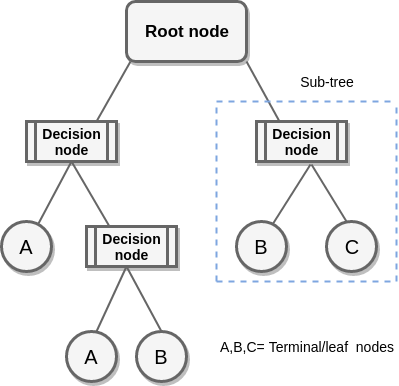
\includegraphics[width=0.6\textwidth]{images/DC.png}
    \caption{An illustration of a decision tree where a recursive partition is shown from the root node where there is an entire data sample to the internal nodes (decision nodes) where splitting occurs to form child nodes, which are either decision nodes or terminal nodes. A terminal node implies that after this split, further splitting of the samples does not provide relevant information in predicting the response variable \citep{moisen2008classification}. }
  \label{images/DecisionTree}
\end{figure}

The binary recursive partitioning applies to the fitting of both classification and regression trees. Each node in a tree is split based on its impurity, which is a measure of how badly the samples at that node fits the model defined in equation \ref{model}. Therefore, in regression and classification trees, variables and the locations of the split are
chosen to minimize the impurity of the node at that point. However, the selection criteria of splitting each node are different for these two methods. In our case the for the regression scenario, the splitting rules used to minimize the impurity of each node $c$ is the MSE and MAE as defined in equations \ref{MSE} and \ref{MAE} \citep{morgan2014classification}. The sample mean of the response variable (estimated value $\mu_{c}$) that represents the assigned prediction in each terminal node is defined as: 
\begin{align}
\mu_{c}=\frac{1}{N_{c}} \sum_{i\in N_{c}} \textbf{Y}_{i},
\label{model}
\end{align} 
where $N_{c}$ is the number of samples in each node, and $\textbf{X}_{c}$ is the training samples. 
 
These methods not only measure the impurity in each node, but are also used to measure the accuracy of the predictor, as in equations \ref{MSE} and \ref{MAE}. Another commonly used strategy or measure in classification problems which also applies in regression problem, for selecting the best splits, from a set of possible split is to maximize the information gain at each tree node; i.e., the split chosen at each decision node is chosen from the the set $\mathrm{argmax (IG(\textbf{X}_{c},s))}$ where $\mathrm{IG}(\textbf{X}_{c},s)$ is the information gain when a split $s$ is applied to sample data $\textbf{X}_c$. This is the difference between the parent node (decision node) impurity and the weighted sum of the child nodes in equation \ref{IG}. 
 
 \begin{align}
 \mathrm{IG}(\textbf{X}_c,s)&= \mathrm{Impurity}(\textbf{X}_c)-\frac{N_{c(\mathrm{left})}}{N_c}\times \mathrm{Impurity}(\textbf{X}_{c(\mathrm{left})})- \frac{N_{c(\mathrm{right})}}{N_c}\times \mathrm{Impurity} (\textbf{X}_{c(\mathrm{right})}), \label{IG}
 \end{align}
 where $s$ is a split partitioning the training sample $\textbf{X}_c$ of size $N_c$ into two datasets $\textbf{X}_{c(\mathrm{left})}$ and $\textbf{X}_{c(\mathrm{left})}$ each of size $N_{c(\mathrm{left})}$ and $N_{c(\mathrm{right})}$.
If the impurity measure is the MSE, we therefore define the information gain by
 \begin{align}
 \mathrm{IG}(\textbf{X}_c,s)&= \mathrm{Impurity}(\textbf{X}_c)-\frac{N_{c(\mathrm{left})}}{N_c}\times \text{MSE}_{(\mathrm{left})}- \frac{N_{c(\mathrm{right})}}{N_c}\times \text{MSE}_{(\mathrm{right})}.
  \end{align}
If the impurity measure is the MAE, the information gain is defined by   
 \begin{align}
 \mathrm{IG}(\textbf{X}_c,s)&= \mathrm{Impurity}(\textbf{X}_c)-\frac{N_{c(\mathrm{left})}}{N_c}\times \text{MAE}_{(\mathrm{left})}- \frac{N_{c(\mathrm{right})}}{N_c}\times \text{MAE}_{(\mathrm{right})}. 
 \end{align}
 
For multi-output decision trees that predict multiple continuous target attributes at once, the advantage over building a separate
regression tree for each target is that the built tree is usually much smaller than the total size of the individual single-target trees for all variables; secondly they identify the dependencies between the different target variables  better.

The building of the multi-output decision trees follows  the same steps as the standard decision tree in Figure \ref{images/DecisionTree}, starting with all instances in the root node, then iteratively finding the optimal split and partitioning the nodes accordingly until a terminal node is reached, given a certain stopping criterion. The only difference  is the redefinition of the impurity measures in equations \ref{MSE} and \ref{MAE} of a node as the sum of the squared error  over a multi-target response. 
\begin{align}
\sum_{k\in d}\frac{1}{N}\left[\sum_{l \in N }\left(\textbf{y}_{k}^{(l)}-\mu^{(l)} \right)^2\right],
\end{align}
where $\mu^{(l)}$ denotes the predicted output for the instance $l$ in each node. Each split is selected to minimize the sum of the squared error such that each terminal leaf of the tree can be characterized by the multivariate mean
of its instances and its defining feature values.

\subsection{Random forest}
While classification and regression trees are powerful methods in and of themselves, much work has been done in machine learning to improve the predictive ability of these tools by combining separate tree models into what is often called ensemble.

A random forest is a combination (ensemble) of decision tree predictors such that each tree depends on the values of a random vector sampled independently and with the same distribution for all trees in the forest, as shown in Figure \ref{random tree} \citep{breiman2001random}. This algorithm  was introduced by \citep{ho1995random} after having noticed that decision trees were limited in their accuracy owing to their inability to grow to arbitrary complexity. This method was not only more accurate, but was less susceptible to overfitting.

 \begin{figure}[H]
  \centering
    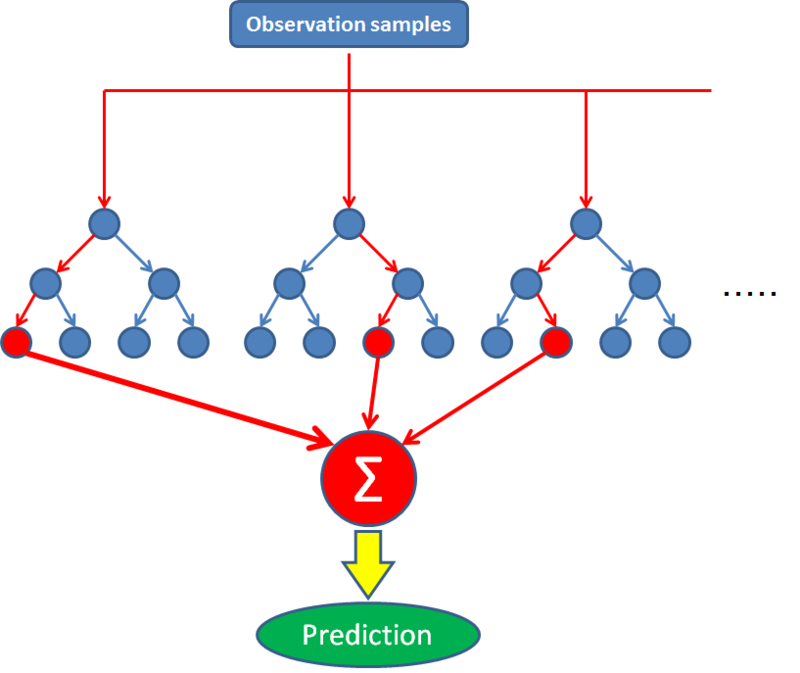
\includegraphics[width=0.6\textwidth]{images/RandomForestTree.png}
    \caption{Random forest regression. [image by Data scientist TJO in Tokyo]}
  \label{random tree}
\end{figure}

During the construction of a component decision tree, at each step
of split selection, a random forest first randomly selects a subset of features, and then carries out the conventional split selection procedure within the selected
feature subset. Note that the randomness is only introduced into
the feature selection process, not into the choice of split points on the selected feature. Random forest is an extension of bootstrap aggregating (bagging), where the major difference with bagging is the incorporation of randomized feature selection \citep{zhou2012ensemble}. The operational procedure of bagging is as follows: 

\begin{itemize}
\item Given a a set $\textbf{X}$ of size $\textit{N}$.
\item Generate $\textit{m}$ subsets in vector $\Theta$  of length $\textit{n}$ by randomly selecting data from the set $\textbf{X}$ with replacement \citep{breiman2001random}. 
\item Run $\textit{k}$ number of trees for each of the $\textit{m}$ sets of $\Theta$ to train the data.
\item This will generate $\Theta_{\textit{m}}$ sets of trained data.
\item For the remaining $\textit{n}$ sample, trained trees from the previous two steps can be fitted onto the remaining
data set of $\textbf{X}_{\textit{n}}$ to estimate the features of the data.
\end{itemize}

The parameter $\textit{k}$ controls the incorporation of randomness and this results in an increase in the bias. When $\textit{k}$ equals the total number of features, the constructed decision tree is identical to the traditional deterministic decision tree, when $\textit{k}$ = 1, a feature will be selected randomly. The suggested value of $\textit{k}$ is the logarithm of the number of features \citep{breiman2001random}.

The predictions of the trees that are constructed by the random forest are aggregated (majority voting for classification or averaging for regression) to produce the final output prediction. Suppose the underlying true function we try to learn is $f(\textbf{x})$, and $\textbf{x}$ is sampled according to a distribution p($\textbf{x}$). The output of each decision tree learner can be written as the the true value plus an error item, i.e.,
\begin{align}
h_{i}(\textbf{x})= f(\textbf{x}) + \epsilon_{i} (\textbf{x}), i = 1, \dots,T.
\label{hx}
\end{align}
such that we have the averaging and, 
\begin{align}
H(\textbf{x})= \frac{1}{T}\sum_{i=1}^{T} h_{i}(\textbf{x}). 
\label{averageRF}
\end{align}
\citep{zhou2012ensemble}

Recall in Section \ref{Dt}, that the prediction of  each tree is the sample mean, then from equation \ref{hx} we thus have the MSE of the output prediction $h_i$ as 
\begin{align}
\int (f(\textbf{x})-h_{i}(\textbf{x}))p(\textbf{x})^2d\textbf{x} = \int \epsilon_{i} (\textbf{x})^2 p(\textbf{x})d\textbf{x}.
\end{align}
Similarly, we can derive the MSE of the combined decision tree learner (i.e., the ensemble) as 

\begin{align}
\int \left(f(\textbf{x}) - \frac{1}{T}\sum_{i=1}^{T} h_{i}(\textbf{x}) \right)^2  p(\textbf{x})d\textbf{x} = \int \left( \frac{1}{T}\sum_{i=1}^{T} \epsilon_{i}(\textbf{x})\right)p(\textbf{x})d\textbf{x}
\end{align} 


The two main parameters of a random forest are the number of trees grown and the number of predictors randomly tried at each split. What one calls depth is sometimes found as the maximum node size, and controls the size of the trees that are grown. In the original implementation of random forest, trees are grown to the maximum potential extent so that they reach the lowest possible bias. Then, variance is reduced by growing many trees and averaging them. The main reason is that in random forest, one can only decrease error by reducing the variance, so the bias needs to be as low as possible in the first place. Therefore, in most cases, one does not really need to adjust this parameter (depth or max nodesize). but just has to make sure the default value allows the trees to grow as deeply as possible.

\subsection{K-nearest neighbour}

The K-nearest neighbor algorithm is a well known non-parametric algorithm commonly used for regression and classification problems. This algorithm does not make any assumptions about the distribution of the data being evaluated, i.e., the model structure is determined from the data. The learning technique used in K-nearest neigbors is known as the instance-based learning. This technique is based on the memorization of the training dataset and the number of parameters is unbounded and grows with the size of the data. 

The intuition underlying nearest neighbor regression is quite straightforward;
the output predictions are obtained by looking into the memorized examples where the cost of the learning process is 0. The cost is in the computation of the prediction, with the prediction output being the continuous average values (or median) of the values of its K-nearest neighbors. The commonly used measure in K-nearest neighbors is the distance functions , i.e., consider $\mathcal{M}$ the m-dimensional Euclidean space $\mathbb{R}^m$  , a training data set $\textbf{X}=\{\textbf{x}_1,\dots, \textbf{x}_n\} \subset \mathcal{M}$, a query point $q\in \mathcal{M}$, and a distance metric $d:\mathcal{M}^2 \rightarrow \mathbb{R}$. The K-nearest neighbor search is the task of finding  the K closest (w.r.t. $d$ ) points to $q$ from the data set $\textbf{X}$, i.e., we find a set $\textbf{A} \subset \textbf{X}$ for which it holds  that $|\textbf{A}|= K$ and  $d(q,\textbf{x})\leq d(q,\textbf{y})$ $\forall$ $\textbf{x}\in \textbf{A}, \textbf{y}\in \textbf{X} \;\text{or}\; \textbf{A}$ \citep{hyvonen2015fast}. 

The distance function is defined as 
\begin{align}
d(\textbf{x},\textbf{y})= \sum_{i=1}^m \left(|x_i -y_i|^m\right)^{\frac{1}{m}}
\end{align}
known as the Minkowski distance. For a special case where $m=1$, the distance function is a Manhantan distance also know as the L-1 norm
\begin{align}
d(\textbf{x},\textbf{y})= \sum_{i=1}^m|x_i -y_i|,
\end{align}
and if $m=2$, the distance function is a Euclidean distance, also know as the L-2 norm and, 
\begin{align}
d(\textbf{x},\textbf{y})= \sqrt{\sum_{i=1}^m \left(x_i -y_i \right)^2}
\end{align}
\citep{cunningham2007k}.

\begin{figure}[H]
  \centering
    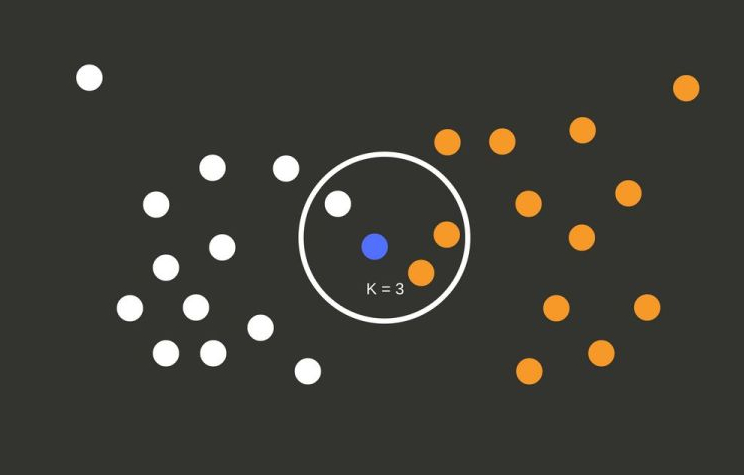
\includegraphics[width=0.5\textwidth]{images/Kn.jpg}
    \caption{Example of K-nearest neighbor. We have two different target classes white and orange circles and a total of 26 training samples. To predict the target class for the blue circle, considering the K value as three, one needs to calculate the similarity distance using similarity measures such as Euclidean distance \citep{K-NNALGORITHM}.}
  \label{kn}
\end{figure}

\subsection{Extremely randomized tree}

Extremely randomized tree is another tree-based ensemble method for supervised classification and regression problems. It builds an ensemble of decision trees according to the classical top-down procedure in Figure \ref{random tree}. Its differences from other tree-based ensemble methods (random forest) are that the nodes are being split by choosing a threshold (cut-point) at random, and that it uses the whole training dataset rather than the bootstrap replica to grow the trees.  

As in random forest, the predictions of the trees are also aggregated to yield the final prediction, by majority vote in classification problems and arithmetic average in regression problems as shown in equation \ref{averageRF}. The explicit randomization of the cut-point and ensemble averaging reduces the variance even more, i.e. $\text{error}=\text{bias} - \text{variance}$ \citep{geurts2006extremely}. 
\section{Training and testing}
\label{TT}
The process of training and testing involves feeding a learning algorithm with training data (seen data) to learn from by finding suitable parameters and evaluate its performance using testing data (unseen), as illustrated in Figure \ref{overview}. A fundamental assumption of machine learning is that the training data are representative of the distribution from which future data  will be chosen \citep{witten2016data}. Each instance in the training set contains "target value" and several "attributes" (namely features). 

\begin{figure}[H]
  \centering
    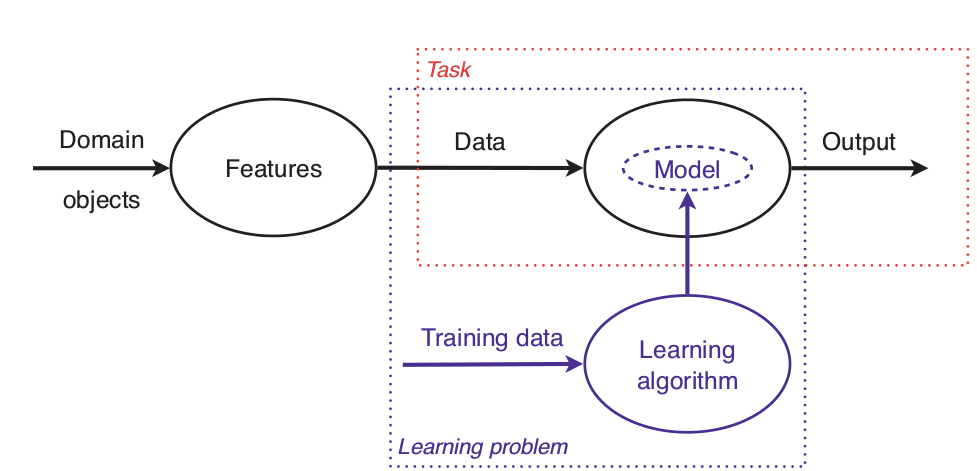
\includegraphics[width=0.7\textwidth]{images/MLSampler.png}
    \caption{An overview of machine learning model training \citep{flach2012machine}.}
  \label{overview}
\end{figure}

Referring to Section \ref{prep}, some challenges and difficulties of gathering  a larger data set were encountered  due to faulty radio telescopes leading to observations being conducted with fewer elements in an array, observations with target of interest PKS1613-586 conducted using only the baselines of interest (short or long), KAT-7's lifespan lasting for a short period, and radio frequency interference affecting calibration solutions. The advantage of having a large testing dataset is a more reliable estimate of accuracy, whereas a large training set is more representative of how much data are available for the learning process. 

Despite the challenges mentioned above, we managed to construct a data matrix $\textbf{M}$ of dimension  $1760\times 75$ containing sensor data $\textbf{X}_t\in \mathbb{R}^{1760 \times 47}$ and 1GC calibration solutions $\textbf{Y}_t$ $\in \mathbb{C}^{1760 \times 14}$ from 28 different observations at integration time $\Delta t$ ranging from $1-12$ hours dependending on each observation requirement. Take note that the 14 columns in plane $\mathbb{C}$ represent the amplitude and phase solutions for H,V polarization, i.e. $7 \times 2$; and the 47 columns in plane $\mathbb{R}$ are the number of selected sensors for all the antennas. Since each calibration solution in $\textbf{Y}_t$ is represented as a complex variable \begin{align}
e^{i\phi}= \cos\phi + i\sin\phi, \label{cx}
\end{align} for each polarization H $\&$ V. Due to different physical causes on the received signal, we therefore choose to treat the antenna phases and amplitudes separately by splitting equation \ref{cx}, into gain amplitude solutions  $\left|e^{i\phi}\right|$ and gain phase solutions $\phi$ in radians for both H $\&$ V. In every supervised machine learning problem, it is crucial to label the input and output of the dataset before starting the learning process. In our case, since this is a regression problem aiming to predict calibration solutions from sensor data, we therefore label the sensor data as input features and the calibration solutions as output targets.
    
\begin{figure}[H]
  \centering
    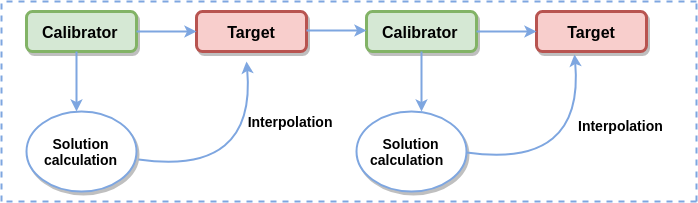
\includegraphics[width=0.7\textwidth]{images/cal4.png}
    \caption{Observation procedure and calibration using CASA}
  \label{Cal2}
\end{figure}

\begin{figure}[H]
  \centering
    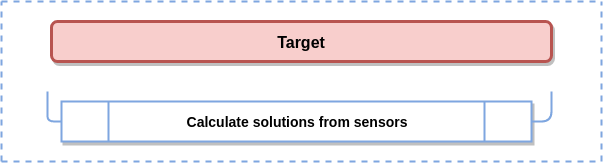
\includegraphics[width=0.7\textwidth]{images/Cal3.png}
    \caption{Observation procedure goal using machine learning}
  \label{Cal3}
\end{figure}

Figure \ref{Cal2} shows the observation procedure of KAT-7 where the calibrator is close to the target source (preferably within the range of $10^{\circ}$ to $15^{\circ}$), with the scan switching  between  the target and the calibrator \citep{taylor1999synthesis}. This is to minimize the phase perturbation caused by atmosphere. The calibration solutions are obtained from the phase calibrator ("green") in Figure \ref{Cal2} at different time intervals $\Delta t$ of tracking called duty cycles. This is done assuming that the calibrator PKS1613-586 has invariant characteristics (i.e. known positions in the sky or known properties from previous observations). One of the standard properties for an ideal instrument would be the $0^{\circ}$ antenna-based gain phase response and constant amplitude for all baselines. In reality this is not always the case because of instrumental defects such as phase and amplitude drifts in the electronics of each antenna; amplitude response as a function of elevation (gain curve), and tropospheric amplitude and phase effects and other external effects. Hence, to calculate the calibration solutions, CASA considers each antenna-based gain $J_i$ and the prior information about the calibrator to perform some adjustments or estimations $G$ over the calibrator's duty cycle $\Delta t$ for all the instruments $i,j$. These solutions at each duty cycle are then temporarily interpolated using the $\textit{interp}$ parameter inside the $\textit{gaincal}$ CASA task. 

%Interpolation is a model based recovery of continuous data from discrete data with known range \citep{thevenaz2000image}. There are different methods of interpolation used, and in this Section, we only look at linear and nearest interpolation which are popular in radio calibration. Example: Assume that we have two known data points $(x_1,y_1,t_1)$ and  $(x_2,y_2,t_2)$ at time $t_1$ and $t_2$, we would like to estimate what $y$ value we would obtain at time $t$ for some point $x$ that is between $x_1$ and $x_2$. For nearest interpolation method, $y$ would be assigned to the value of the nearest point of $x$. For linear interpolation method, a line is fitted between the points $(x_1,y_1,t_1)$ and $(x_2,y_2,t_2)$  and we look to see the value of $y$ in a line for our chosen $x$ at time $t$. The points $x_1,\dots, x_n$ are called the interpolation points. The property of passing
%through these points is referred to as interpolating the data and the function that interpolates the data is an interpolant \citep{levy2010introduction}. An example of interpolation is further illustrated in the following Figure \ref{int}. 
%
%  \begin{figure}[H]
%  \centering
%    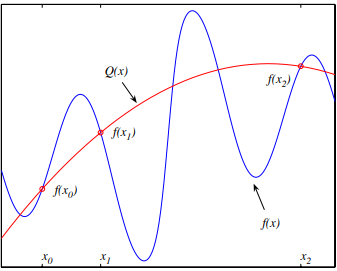
\includegraphics[width=0.5\textwidth]{images/Int.png}
%    \caption{Given a function $f(x)$ with distinct points $x_0<x_1,<x_2,\dots <x_n$ at $n+1$. The interpolation problem is to construct a function $Q(x)$ that passes through these points, i.e, to find a function $Q(x)$ such that the requirements $Q(x_i)=f(x_i)$, $0\leq i\leq n$ are satisfied \citep{levy2010introduction}.}
%  \label{int}
%\end{figure}
 
After obtaining solutions $G$, they are written into calibration tables and later applied to the target source of interest, $T$. The CASA task for this process is called $\textit{applycal}$, which reads the specified calibration tables, applies them to the observed data column through an interpolation process at each single time unit for different target duty cycles $\Delta t, \Delta t_{n+1},\dots$, following the order shown in Figure \ref{Cal2}. The calibrated results are then written into the corrected column for imaging or other scientific processing \citep{ott2013casa}. Since CASA "calculates" the solutions using interpolation and estimation methods given some prior information about the calibrators, the goal of the experiment is to produce a model (based on the training data) that learns the behaviour and changes of the calibrator owing to various external effects and able to predict the calibration solutions of the test data with high accuracy, given only the test sensors at different duty cycles. This will help in speeding up the calibration processes and decreasing the time duration for tracking the phase calibrator PKS1613-586 and therefore increasing the time duration for tracking the target observed as shown in Figure \ref{Cal3}. 

Since the sensor data obtained from the radio telescope are of different scales, i.e., unstructured. a pre-processing stage before proceeding with the training of the learning algorithms is necessarily. We propose to use a scaling statistical technique called Z-score normalization or standardization. This technique gives the normalized values or range of data from the original unstructured data using the concept of mean and standard deviation \citep{patro2015normalization}. The features are rescaled such that they have properties of a standard normal distribution with mean $\mu=0$ and standard deviation $\sigma=1$. 
\begin{align}
Z=\frac{\textbf{x}- \mu}{\sigma}
\end{align}
with mean:
\begin{align*}
\mu= \frac{1}{N} \sum_{j\in N} (\textbf{x}_j),
\end{align*}

and standard deviation:
\begin{align*}
\sigma=\sqrt{ \frac{1}{N} \sum_{j\in N} (\textbf{x}_j-\mu )^2}
\end{align*}
Normalizing the features so that they are centered around 0 with a standard deviation of 1 is not only important if one is comparing measurements that have different units, but is also a general requirement for many machine learning algorithms as this will be helpful for prediction \citep{bott2014feature}.

When training a learning algorithm  in machine learning, two main things might happen as described in Section \ref{comp}, namely overfitting and underfitting. To avoid these, we split the data into two subsets, i.e., training and testing data sets using the $\textit{scikit-learn}$ train-test split strategy \citep{buitinck2013api}. 

  \begin{figure}[H]
  \centering
    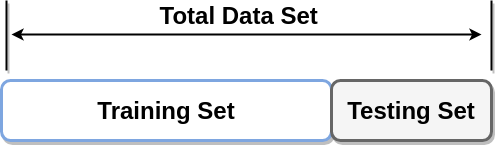
\includegraphics[width=0.7\textwidth]{images/t_s.png}
    \caption{This is a train-test split strategy where a data matrix is randomly split into training and testing  subsets.}
  \label{ts}
\end{figure}

From Figure \ref{ts}, once the data have been normalized, we perform a 80$ \%$ training and 20$\%$ testing split. The training set contains a known output and the model will learn using these data in order to be generalized to other data later on. The test dataset is used to test the model's prediction on this subset.
 
Model training in machine learning requires tuning of the  hyper-parameters that determine the behaviour of the learning algorithm and hence the performance
of the resulting model on unseen data. This involves finding the best combination of hyper-parameters with respect to the user-specified criterion \citep{buitinck2013api}. For this task, we make use of a randomized search cross-validation (RandomizedSearchCV) function by $\textit{scikit-learn}$ library. This library provides efficient and well-established machine learning tools in
a programming environment that is accessible to non-machine learning experts and reusable in various scientific areas \citep{buitinck2013api}. In a randomized search cross-validation algorithm, not all hyper- parameters are tried out; instead it samples a fixed number of hyper-parameters from a specified probability distribution. i.e., given a set of parameters, $p_i$, each with $N_i$ different values, search all combinations $\prod_i N_i$ with random sampling.
%
%
   \begin{figure}[H]
  \centering
    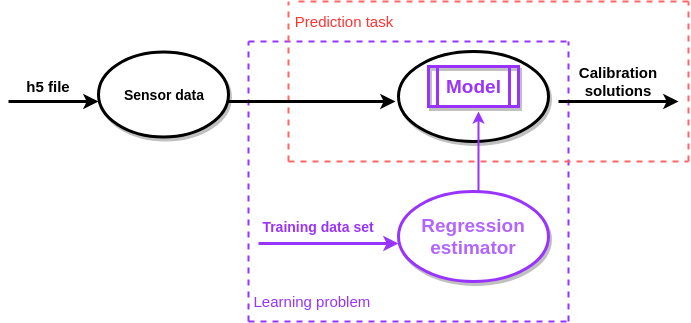
\includegraphics[width=0.7\textwidth]{images/RegressionEST.png}
    \caption{Regression learning diagram showing how we built a regression model estimator by taking in an observation file as input and extracting the sensor data per calibrator scan to obtain an accurate model that predict calibration solutions.}
  \label{DD}
  \end{figure} 


  \begin{table}[H]
\begin{center}
\begin{tabular}{| c | c | c | c | c | c |  }
\hline
 \multicolumn{6}{ |c|}{\textbf{Decision tree estimator $p_i$}} \\ \hline
splitter & max features & min sample split & min sample leaf & max depth & cv\\ \hline
[best,random]&[log2& $\{p_i: 30 \leq p_i \leq 60 \}$& $\{p_i: 7 \leq p_i \leq 14 \}$  & $\{p_i: 700 \leq p_i \leq 1389 \}$ & 10\\ 
&sqrt& & &  &\\
&auto]& & &  &\\ \hline

\end{tabular}
\end{center}
\caption{Decision hyper-parameters} \label{DC_table}
\end{table}


  \begin{table}[H]
\begin{center}
\begin{tabular}{| c | c | c | c | c |  }
\hline
 \multicolumn{5}{ |c|}{\textbf{Random forest estimator $p_i$}} \\ \hline
 n-estimators &max features & max depth & min sample leaf& cv\\ \hline
$\{p_i: 100 \leq p_i \leq 1200 \}$&[log2& $\{p_i: 20 \leq p_i \leq 200 \}$  & $\{p_i: 3 \leq p_i \leq 50 \}$ & 10\\ 
&sqrt& & &  \\
&auto]& & &\\ \hline

\end{tabular}
\end{center}
\caption{Random forest hyper-parameters} \label{RF_table}
\end{table}


 \begin{table}[H]
\begin{center}
\begin{tabular}{| c | c | c | c | c |  }
\hline
 \multicolumn{5}{ |c|}{\textbf{Extremely randomized estimator $p_i$}} \\ \hline
 n-estimators &max features & max depth & min sample leaf& cv\\ \hline
$\{p_i: 100 \leq p_i \leq 1200 \}$&[log2 & $\{p_i: 20 \leq p_i \leq 200 \}$  & $\{p_i: 3 \leq p_i \leq 50 \}$ & 10\\ 
&sqrt& & &  \\
&auto]& & &  \\ \hline

\end{tabular}
\end{center}
\caption{Extremely randomized tree hyper-paramaters}\label{EX_table}
\end{table}

Note that since the random forest estimator \ref{RF_table} and extremely randomized estimator 
\ref{EX_table} are tree-based algorithms, they share the same hyper-parameters as the decision tree estimator \ref{DC_table}, where 
\begin{enumerate}
\item \textit{splitter}: is the strategy used to choose the split at decision node, with $p_i$ best representing the best split and random representing the random split.

\item \textit{max features}: defines the maximum number of features to be considered in the tree when making the best split. The best parameters $p_i$ to choose from are : 
\begin{itemize}
\item if $p_i$ is $\log_2$ then the maximum features is  $\log_2\left(\textit{max features} \right)$

\item if $p_i$ is sqrt then the maximum features is $\sqrt{\textit{max features}}$ 
\item if $p_i$ is auto, then this will simply take all the features that make sense in every tree. Here we simply do not put any restrictions on the individual tree. 
\end{itemize}
\item \textit{min sample split}: denotes the minimum number of samples required for a split in each decision node.
\item \textit{max depth}: denotes the maximum depth of the tree, i.e. determines how deeply the tree should expand. If no parameter is given, then nodes are expanded until all leaves are pure or until all leaves contain less than min samples split.

\item \textit{min sample leaf}: denotes the number of samples required for a node to be a terminal node (leaf node).
\item \textit{n-estimator}: denotes  the number of trees  to be built before taking the maximum voting or averages of predictions. A higher number of trees give better performance but make decrease the speed of processing.
\item \textit{cv}: denotes the cross-validation generator inside RandomizedSearch, which determines the cross-validation strategy, if $p_i$ is an integer, then the number of folds in a KFold are specified \citep{pedregosa2011scikit}. 
\end{enumerate}


\begin{table}[H]
\begin{center}
\begin{tabular}{| c | c | c | c | c | c |  }
\hline
 \multicolumn{6}{ |c|}{\textbf{K-nearest neighbor estimator $p_i$}} \\ \hline
n-neighbors & weights & algorithm & leaf size & p & cv\\ \hline
$\{p_i: 20 \leq p_i \leq 200 \}$&[uniform,distance]&  [auto&$\{p_i: 30 \leq p_i \leq 150 \}$  & [2,3] & 10\\
&&  ball-tree&  &  &\\
&&  kd-tree&  &  &\\ 
&&  brute]&  &  &\\ \hline
\end{tabular}
\end{center}
\caption{K-nearest neigbor hyper-parameters} \label{KNN_table}
\end{table}

One of the most attractive features of the K-nearest neighbor algorithm is that is simple to understand and easy to implement. As shown in Table \ref{KNN_table}, few hyper parameters $p_i$ are tried out, hence it is called a lazy learning algorithm. 

\begin{enumerate}

\item \textit{n-neighbors}: denotes the number of the  K-nearest neighbors of the unknown observation. When K is small, one restrains the region of a given prediction and forces the predictor to limited in seeing the overall distribution, and a higher K averages more voters in each prediction and hence is more resilient to outliers.  
\item \textit{weights}: denotes the weight contribution of each point to the prediction of a query point in the local neighborhood.  
\begin{itemize}

\item If weight $=uniform$, then all points are weighted  equally.
\item If weight $=distance$, then the weights proportional to the inverse of the distance from the query point is assigned.  
\end{itemize}
\item \textit{algorithm}: specifies which algorithm  should be used to compute the nearest neighbors and takes in values such as:
\begin{itemize}

\item If the algorithm is auto, then the algorithm attempts to determine the best approach from the training data.

\item the ball-tree, kd-tree algorithm are used to implement the ball tree algorithm. These data structures are used for fast high-dimensional nearest-neighbor searches.  
\item the brute algorithm is used to implement the brute-force search algorithm. 
\end{itemize}
\item \textit{leaf size}: leaf size is passed to the ball-tree or kd-tree approach for finding k-nearest neighbors in.

\item \textit{p}: denotes the power parameter for the Minkowski metric \citep{pedregosa2011scikit}.
\end{enumerate}

With the number of iterations $\text{n-iter}=50$ RandomizedSearchCV algorithm used to search through, the best estimator obtained, which is the instantiation
mechanism of objects and exposes a fit method for learning a model from
training data for each learning algorithm, is:   
\begin{tcolorbox}
\begin{verbatim}

DecisionTreeRegressor(criterion='mse', 
                      max_depth=890,       
                      max_features='log2',
                      max_leaf_nodes=None,
                      min_impurity_split=1e-07,
                      min_samples_leaf=13, 
                      min_samples_split=30,
                      min_weight_fraction_leaf=0.0, 
                      presort=False, 
                      random_state=0,
                      splitter='best')
\end{verbatim}
\end{tcolorbox}
\begin{figure}[H]
\centering 
\begin{tabular}{l*{8}{c}r}
\hline
            & max-depth &max features&min samples leaf & min samples split  &splitter& score \\
\hline
optimized $p_i$  & 890 & $\log_2$ & 13 & 30 & best&0.686  \\
\end{tabular}
\caption{Decision tree optimized hyper-parameters }
\end{figure}
\begin{tcolorbox}
\begin{verbatim}
RandomForestRegressor(bootstrap=True,
                      criterion='mse',
                      max_depth=90,
                      max_features='auto',
                      max_leaf_nodes=None,
                      min_impurity_split=1e-07,
                      min_samples_leaf=3,
                      min_samples_split=2,
                      min_weight_fraction_leaf=0.0,
                      n_estimators=700,
                      n_jobs=1, 
                      oob_score=0,
                      random_state=0,
                      verbose=0,
                      warm_start=False)
\end{verbatim}
\end{tcolorbox}
\begin{figure}[H]
\centering 
\begin{tabular}{l*{8}{c}r}
\hline
            & max-depth &max features&min samples leaf &n-estimators & score \\
\hline
optimized $p_i$  & 90 & auto & 3 & 700 & 0.902 \\
\end{tabular}
\caption{Random forest optimized hyper-parameters }
\end{figure}
\begin{tcolorbox}
\begin{verbatim}
KNeighborsRegressor(algorithm='brute',
                    leaf_size=30, 
                    metric='minkowski',
                    metric_params=None,
                    n_jobs=1,
                    n_neighbors=20,
                    p=3,
                    weights='distance')
\end{verbatim}
\end{tcolorbox}
\begin{figure}[H]
\centering 
\begin{tabular}{l*{8}{c}r}
\hline
            & algorithm &n-neighbors&p &weights \\
\hline
optimized $p_i$ &brute&20& 3 & distance \\
\end{tabular}
\caption{KNN optimized hyper-parameters }
\end{figure}
\begin{tcolorbox}
\begin{verbatim}
ExtraTreesRegressor(bootstrap=False, 
                    criterion='mse',
                    max_depth=90,
                    max_features='auto',
                    max_leaf_nodes=None,
                    min_impurity_split=1e-07,
                    min_samples_leaf=3,
                    min_samples_split=2, 
                    min_weight_fraction_leaf=0.0,
                    n_estimators=700,
                    n_jobs=1, 
                    oob_score=0,
                    random_state=0,
                    verbose=0, warm_start=False)
\end{verbatim}
\end{tcolorbox}

\begin{figure}[H]
\centering 
\begin{tabular}{l*{8}{c}r}
\hline
            & max-depth &max features&min samples leaf &n-estimators& score \\
\hline
optimized $p_i$  & 90 & auto & 3 & 700 &0.905 \\
\end{tabular}
\caption{Extremely randomized tree optimized hyper-parameters }
\end{figure}

\subsection{Feature importance}
Random forests and extremely randomized trees are well established ensembles of tree models that not only produce good predictive performance, but also provide rich feature importance information \citep{kazemitabar2017variable}. Generally, importance provides a score that indicates how  valuable each feature was in the construction of the decision trees in the model. Importance is calculated for a single decision tree by the amount that each split point improves the performance measure, weighted by the number of observations the node is responsible for. The performance measure can be the average of the impurity reductions over all nodes in the tree where a split was made on that variable, with impurity reductions weighted to account for the size of the node \citep{kazemitabar2017variable}.

\begin{figure}[H]
  \centering
    \includegraphics[width=0.8\textwidth]{images/FeatureSpace.eps}
    \caption{Feature importance}
    \label{FI}
\end{figure}
Figure \ref{FI} shows the importance of each feature in each learning algorithm i.e. the values with the highest contribution in building an accurate model. One observes that the environmental features air temperature, relative humidity, wind speed, wind direction and air pressure are higher ranked than the pointing sensors. The pointing features are ranked second, with the telescope elevation sensors being higher than the telescope azimuth sensors. 

\section{Results}
\label{sec3}
This section shows the plots of the predictions for the decision tree, random forest, extremely randomised trees and the K-nearest neighbor. The algorithms are run a number of times on the learning sample and tested on the test samples to estimate the prediction errors. 
\subsection{Decision tree-RUN}
\begin{figure}[H]
   \centering
    \begin{subfigure}[t]{0.52\textheight}
        
        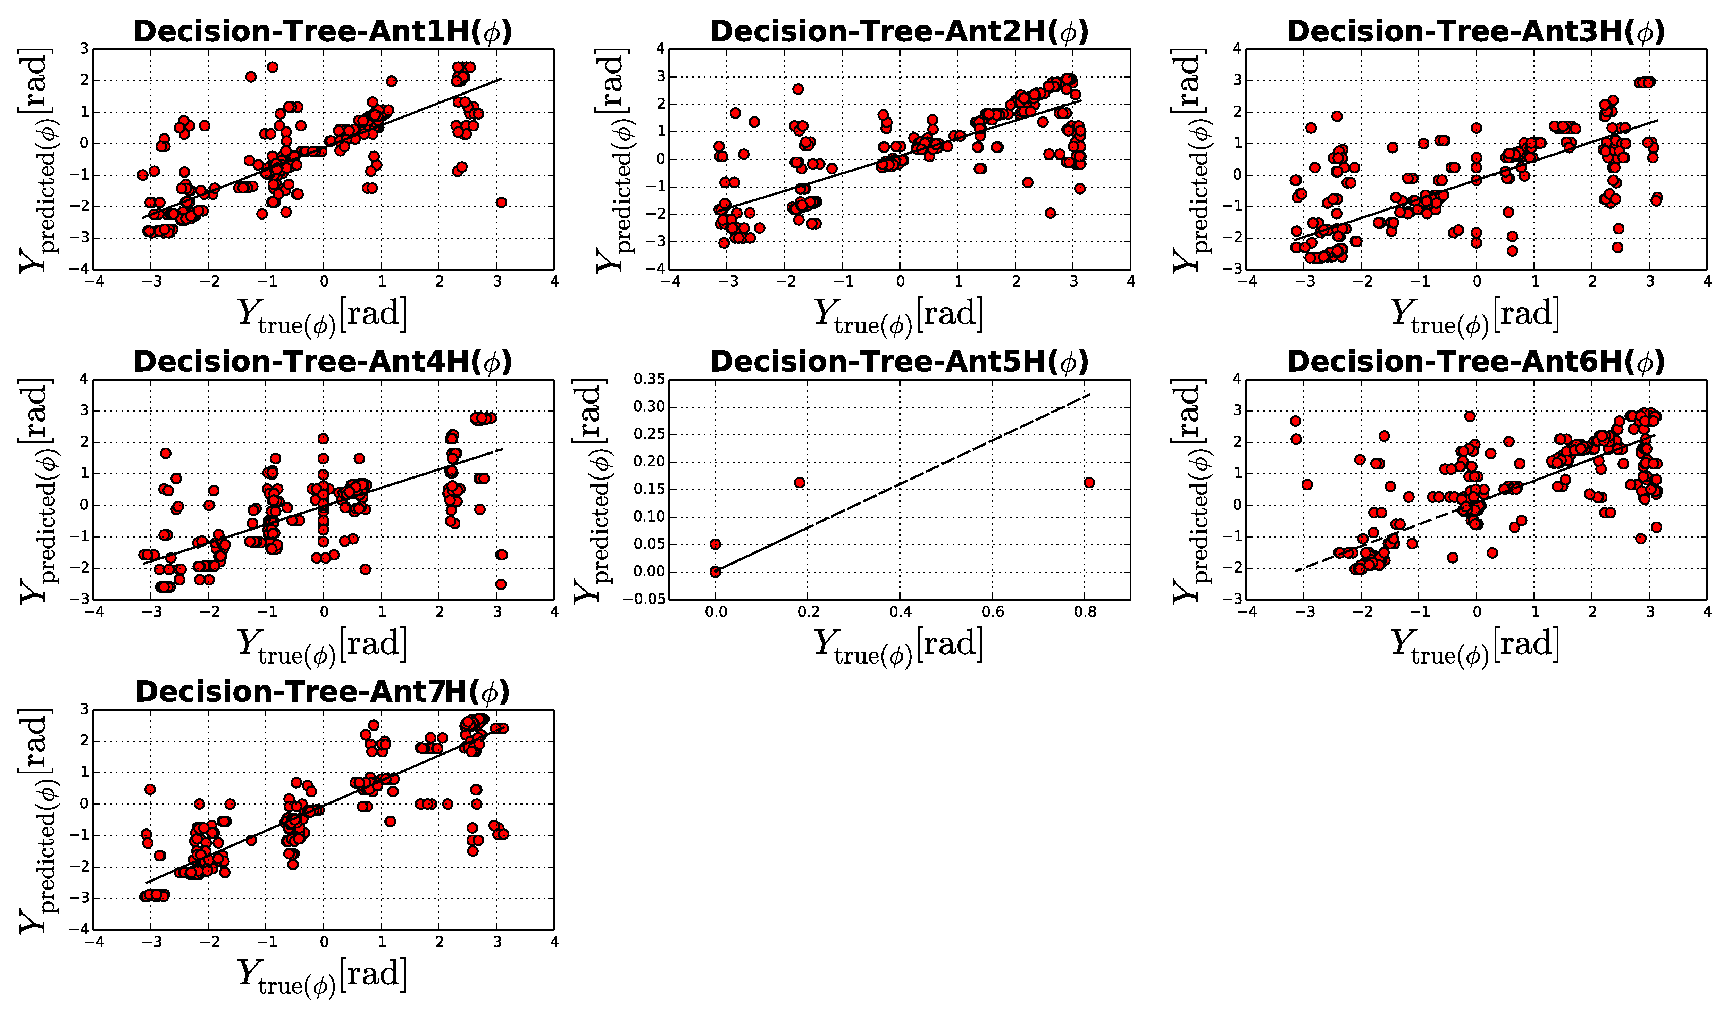
\includegraphics[width=\textwidth]{images/Decision-TreeHphase.eps} 
        \caption{Phase gain solutions for H-polarization}
         \label{A}
    \end{subfigure}
    
      \begin{subfigure}[t]{0.52\textheight}
       
        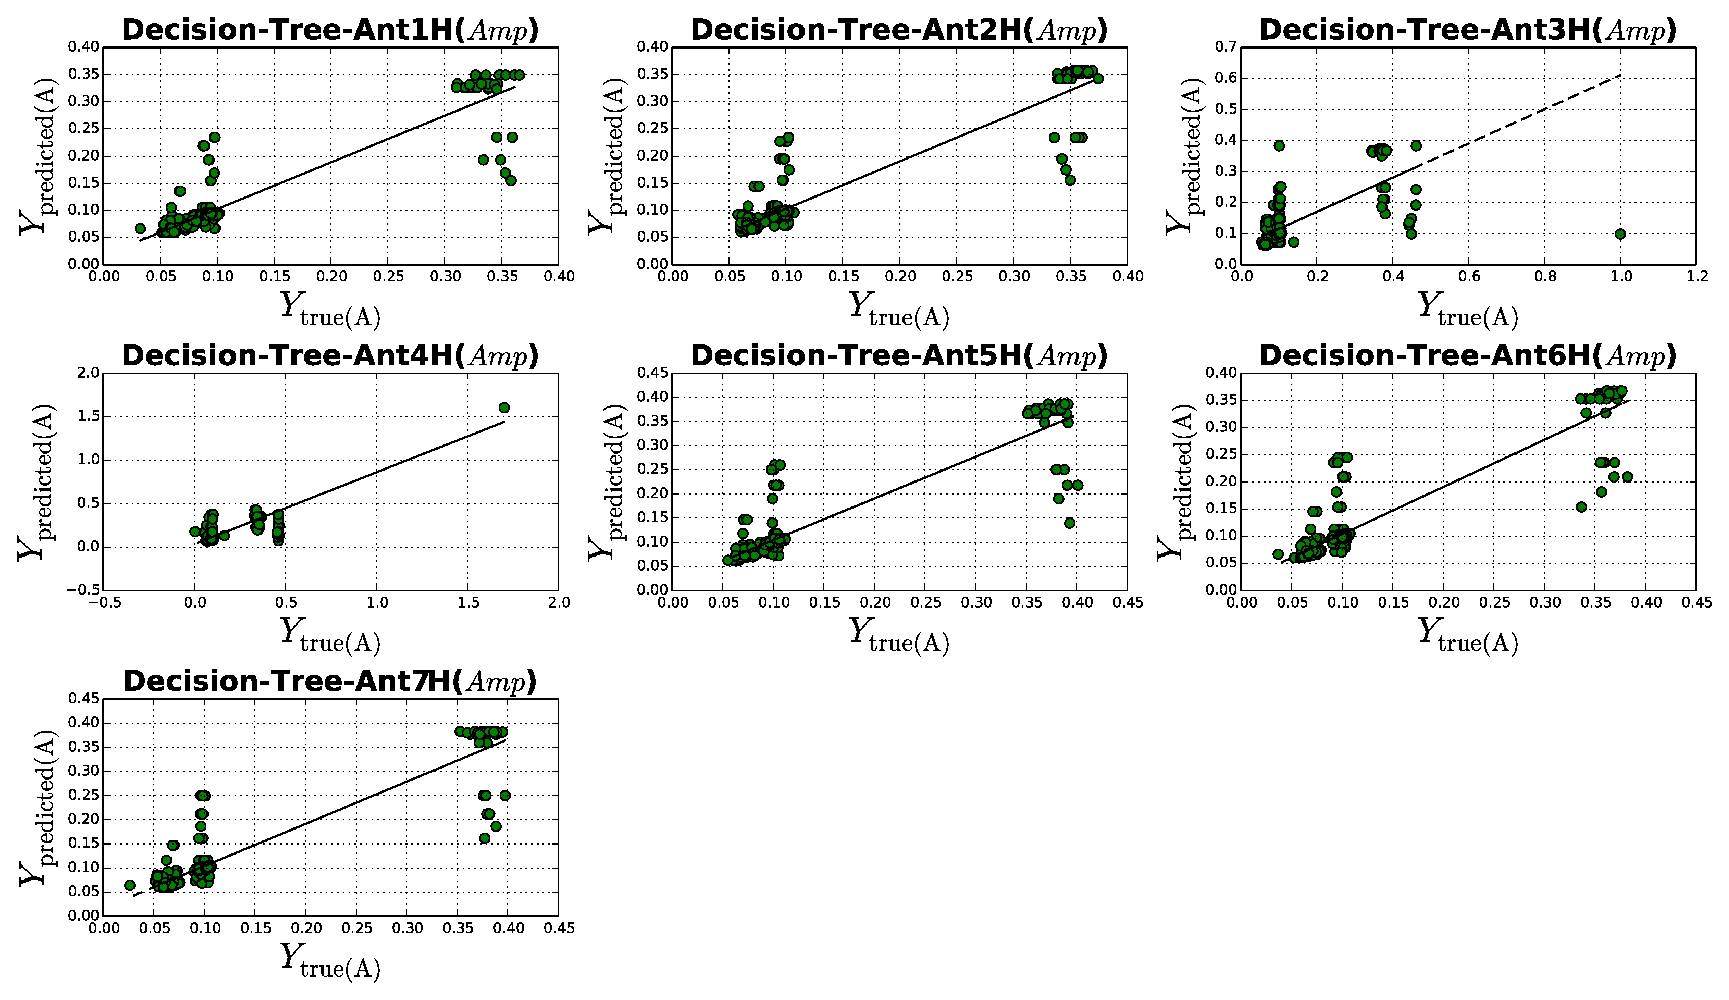
\includegraphics[width=\textwidth]{images/Decision-TreeHamp.eps} 
        \caption{Amplitude gain solutions for H-polarization.}
         \label{B}
    \end{subfigure}
    \caption{Results obtained from the decision tree learning algorithm with randomized search optimization algorithm. (\subref{A}) and (\subref{B})are the predicted gain solutions $\textbf{Y}_{predicted}$ by the decision tree vs the true gain solutions $\textbf{Y}_{true}$ (CASA) for H-polarization. We observe that the decision tree algorithm is performing bad in predicting the H-polarization amplitude and phase gain solutions}
 \label{BB}
    \end{figure}
  
\begin{figure}[H]
   \centering
    \begin{subfigure}[t]{0.52\textheight}
        
        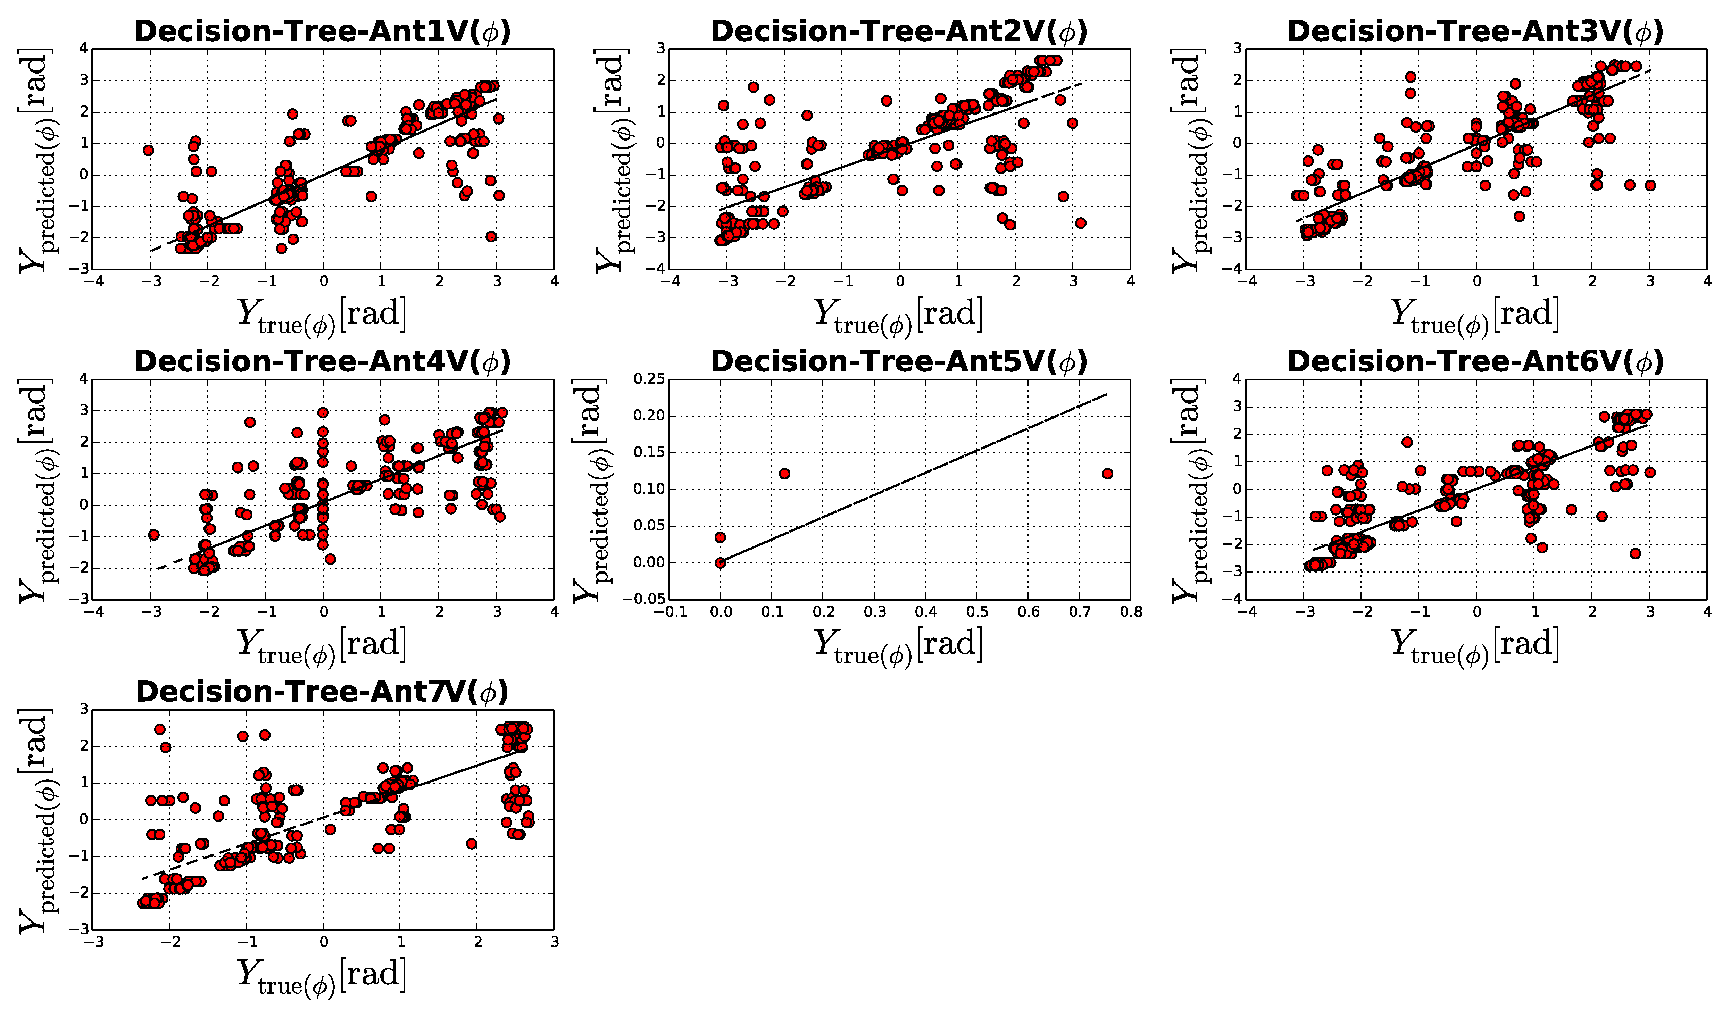
\includegraphics[width=\textwidth]{images/Decision-TreeVphase.eps} 
        \caption{Phase gain solutions for V-polarization}
         \label{A1}
    \end{subfigure}
    
      \begin{subfigure}[t]{0.52\textheight}
       
        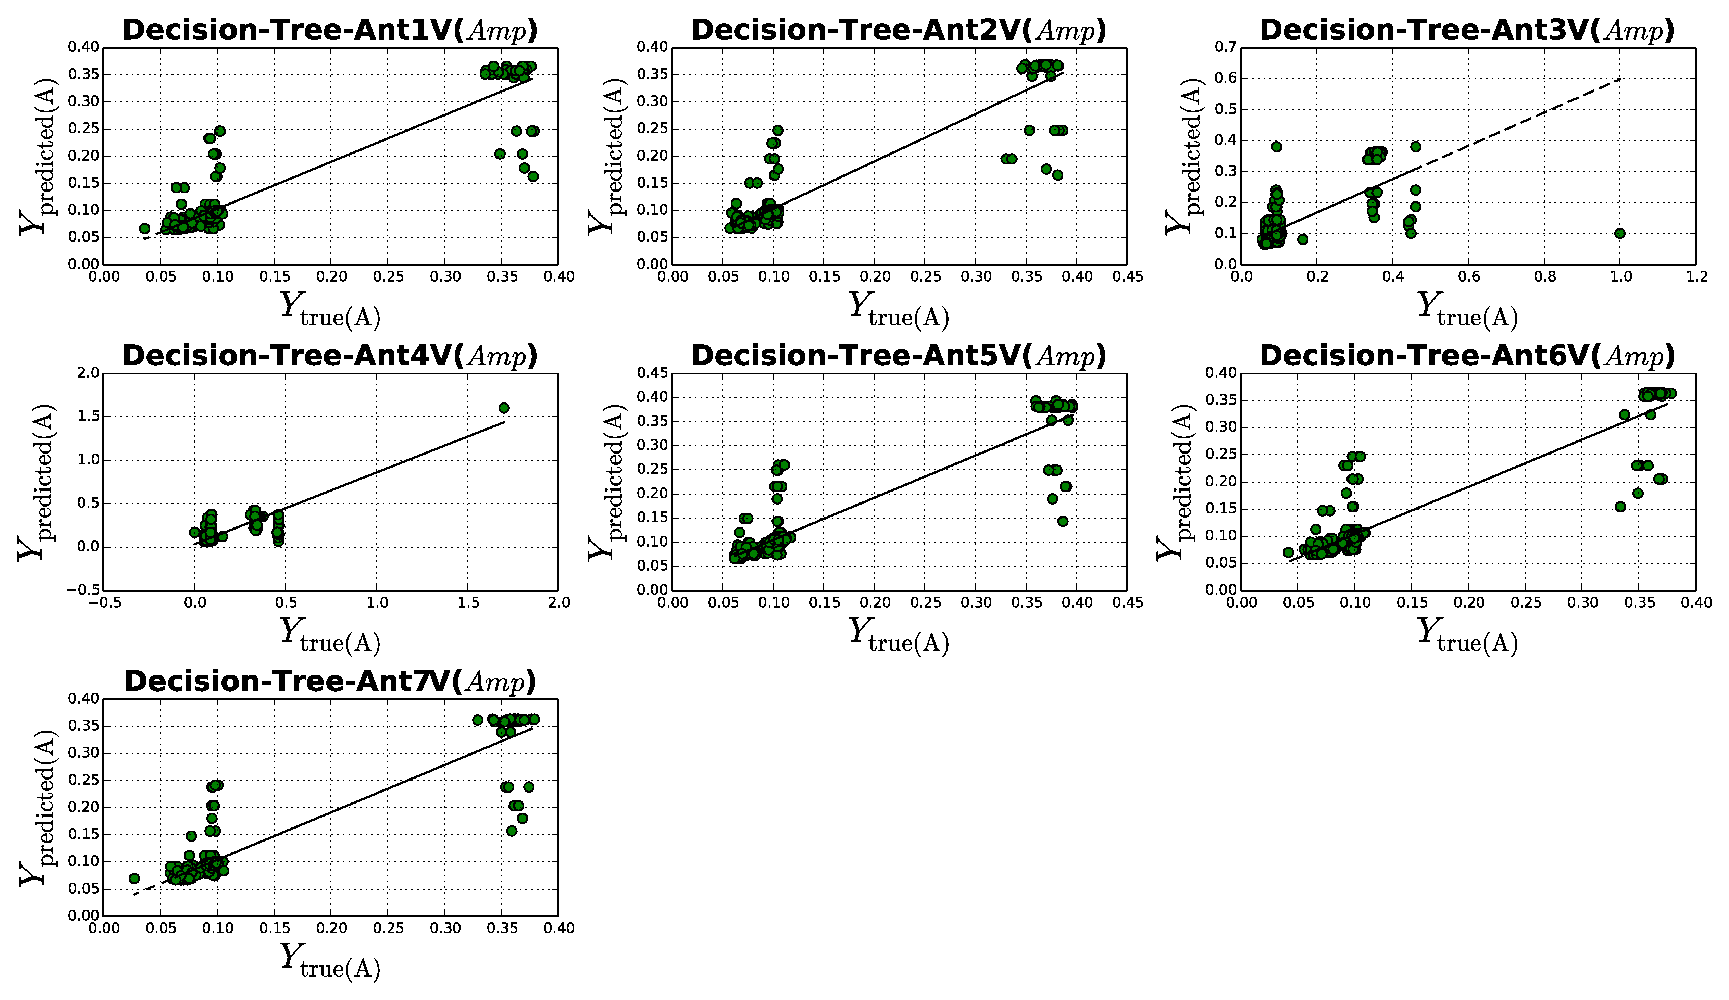
\includegraphics[width=\textwidth]{images/Decision-TreeVamp.eps} 
        \caption{Amplitude gain solutions for V-polarization} 
        \label{B1}
    \end{subfigure}
    \caption{Results obtained from the decision tree learning algorithm with randomized search optimization algorithm. (\subref{A1}) and (\subref{B1}) are the predicted gain solutions $\textbf{Y}_{predicted}$ by the decision tree vs the true gain solutions $\textbf{Y}_{true}$ (CASA) for V-polarization. Similar to H-polarization above, the decision tree algorithm is failing to predict V-polarization amplitude and phase gain solutions.}
 \label{BB1}
    \end{figure}
    
\begin{table}[H]
\label{T:equipos}
\begin{center}
\scalebox{0.7}{
\begin{tabular}{| c | c | c | c | c |}
\hline
Antenna & \multicolumn{4}{ c |}{\textbf{Decision tree phase}}  \\ 
\cline{2-5}
&Rmse & Rmae & R2score &Explained $\sigma^2$\\
\hline
Uniform average-H &0.573 & 0.417 & 0.820   & 0.821 \\ 
Uniform average-V &0.435 & 0.367 & 0.879    & 0. 879\\ \hline
 & \multicolumn{4}{ c |}{\textbf{Decision tree amplitude}}  \\ 
\cline{1-5}
\hline
Uniform average-H &0.043 & 0.109 & 0.835   & 0.835 \\ 
Uniform average-V &0.043 & 0.109 & 0.831    & 0.831\\\hline
\end{tabular}}
\end{center}
\caption{The table shows the performance of the decision tree algorithm in predicting the amplitude and phase gain solutions for both H and V polarizations as shown in Figures \ref{BB} and \ref{BB1}. The values shown represent uniform average of all KAT-7 antennas, i.e., all output measures are averaged with uniform weight. Most of the predictions scatter away from the ideal truth values.}
\end{table}

\subsection{Random forest-RUN}
\begin{figure}[H]
   \centering
    \begin{subfigure}[t]{0.52\textheight}
        
        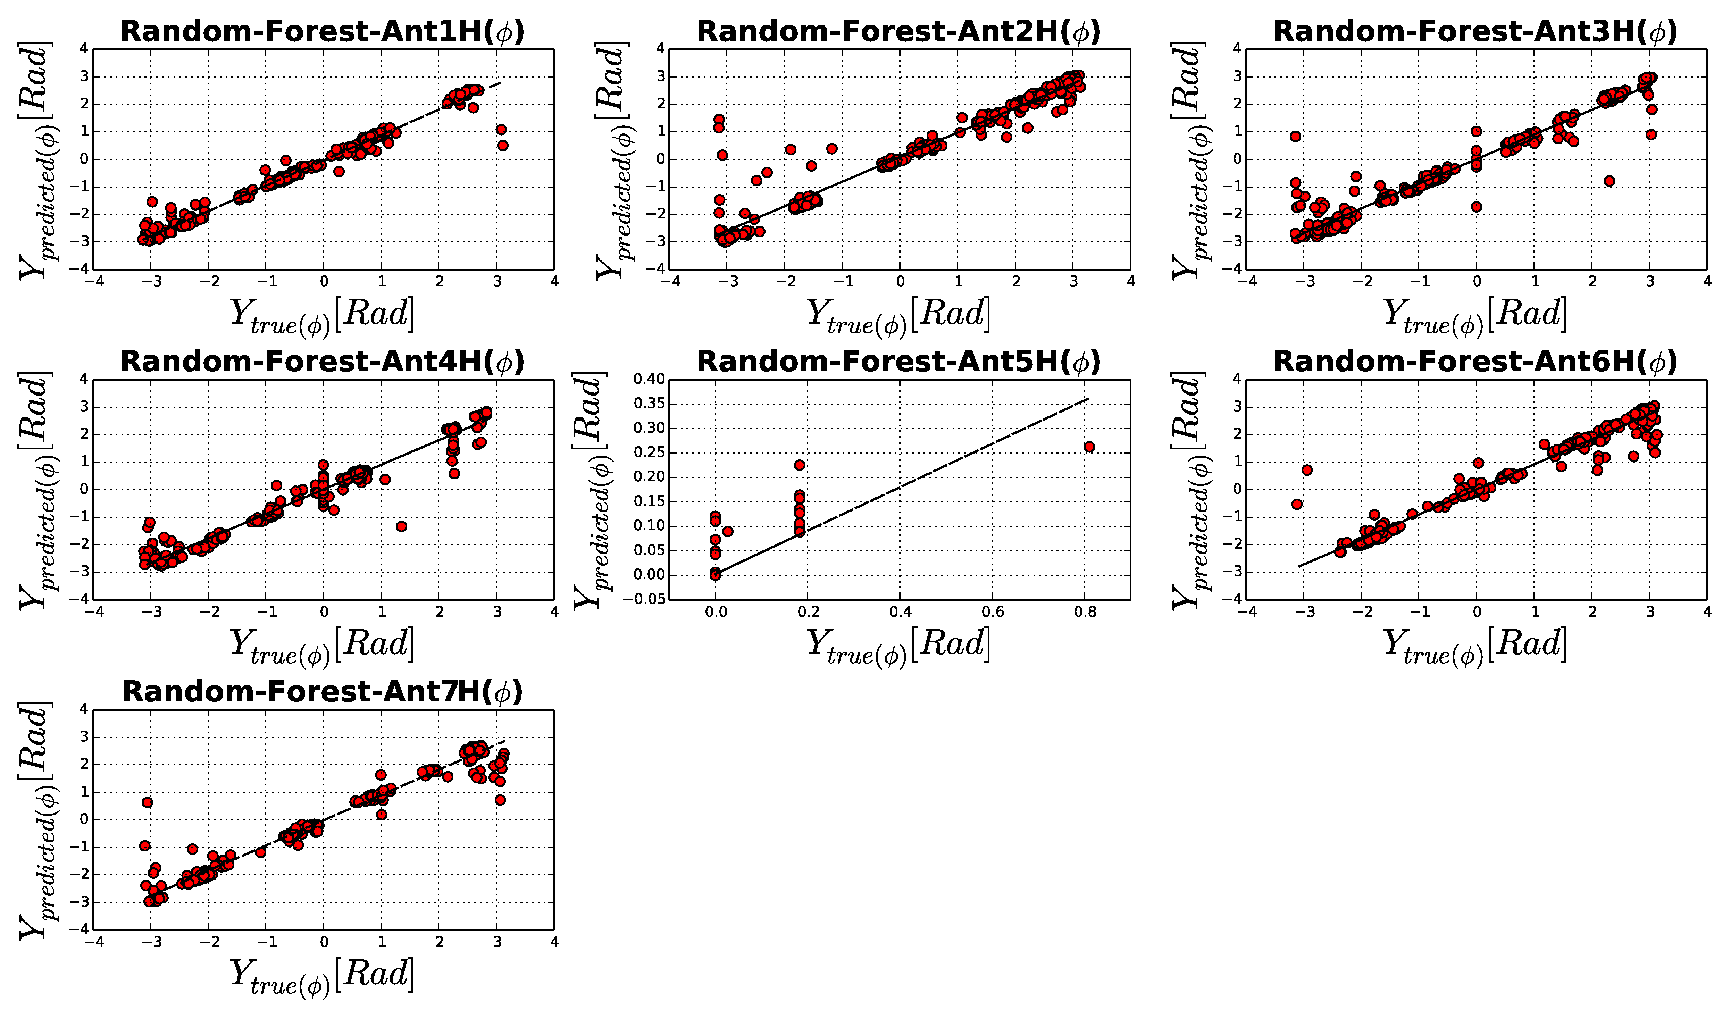
\includegraphics[width=\textwidth]{images/Random-ForestHphase.eps} 
        \caption{Phase gain solutions for H-polarization} \label{A2}
    \end{subfigure}
    
      \begin{subfigure}[t]{0.52\textheight}
       
        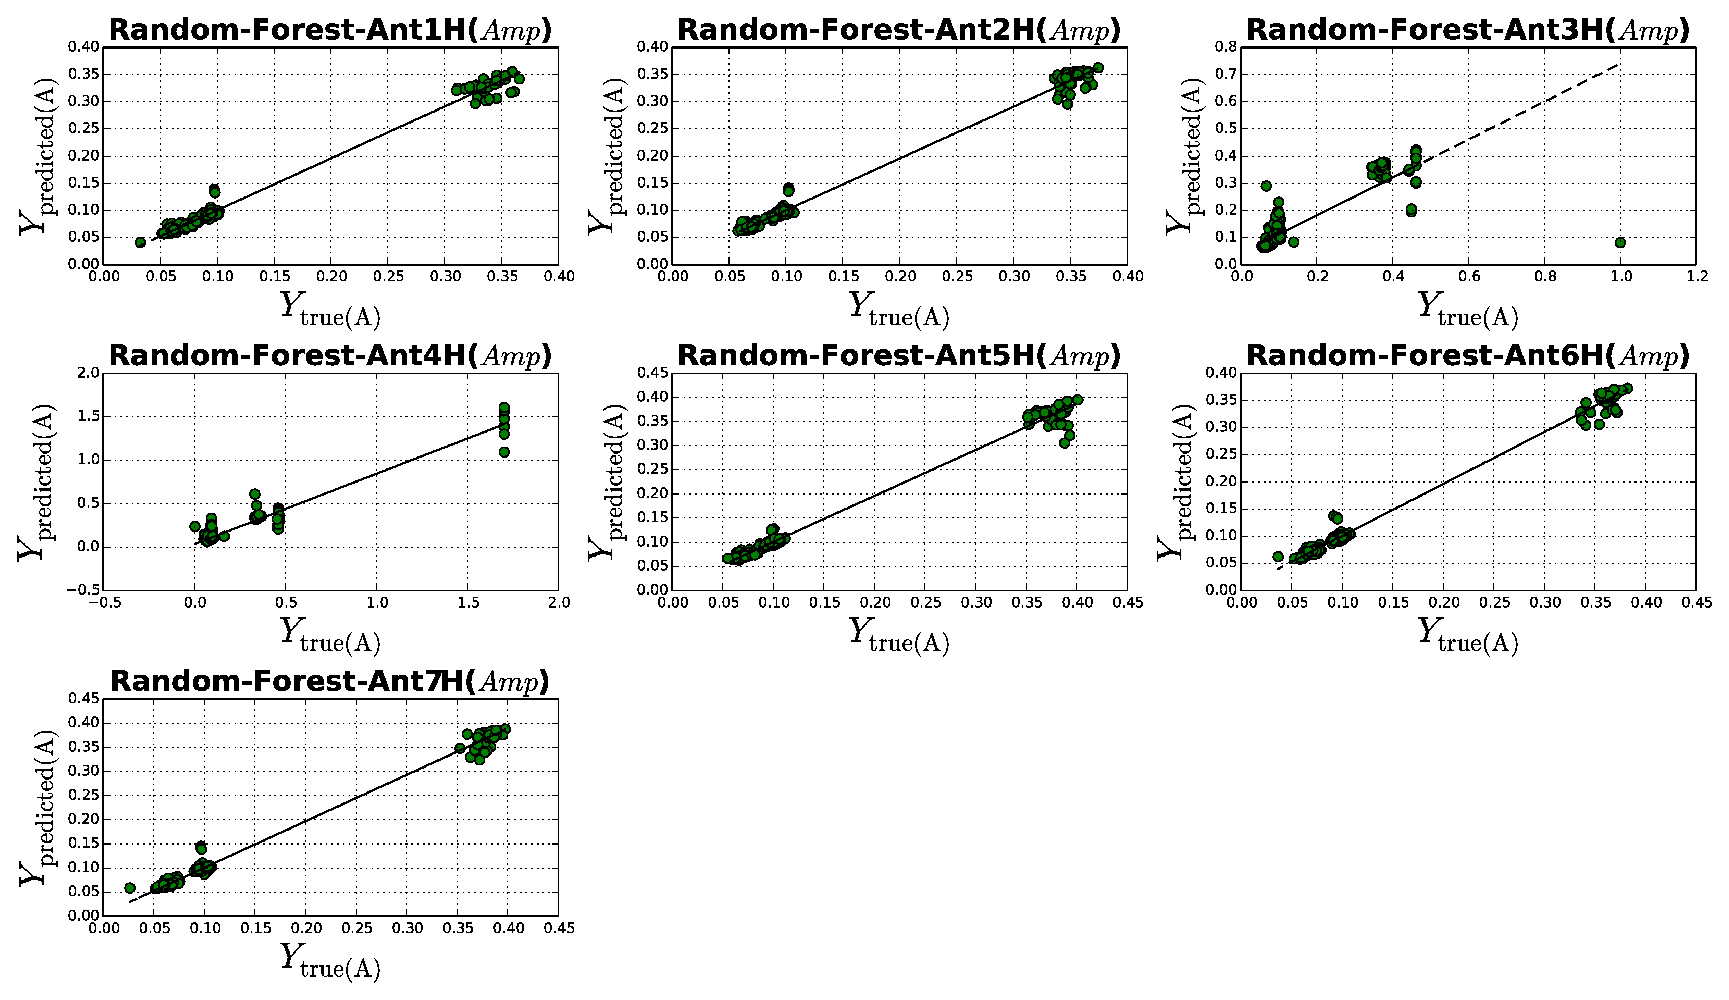
\includegraphics[width=\textwidth]{images/Random-ForestHamp.eps} 
        \caption{Amplitude gain solutions for H-polarization} \label{B2}
    \end{subfigure}
    \caption{Results obtained from the random forest learning algorithm with randomized search optimization algorithm. Figures (\subref{A2}) and (\subref{B2}) are the predicted gain solutions $\textbf{Y}_{predicted}$ by the random forest vs the true gain solutions $\textbf{Y}_{true}$ (CASA) for H-polarization. We observe that the random forest algorithm is performing better in predicting the H-polarization amplitude and phase gain solutions with few outlier points.}
    \label{BB2}
    \end{figure}
    
\begin{figure}[H]
   \centering
    \begin{subfigure}[t]{0.52\textheight}
        
        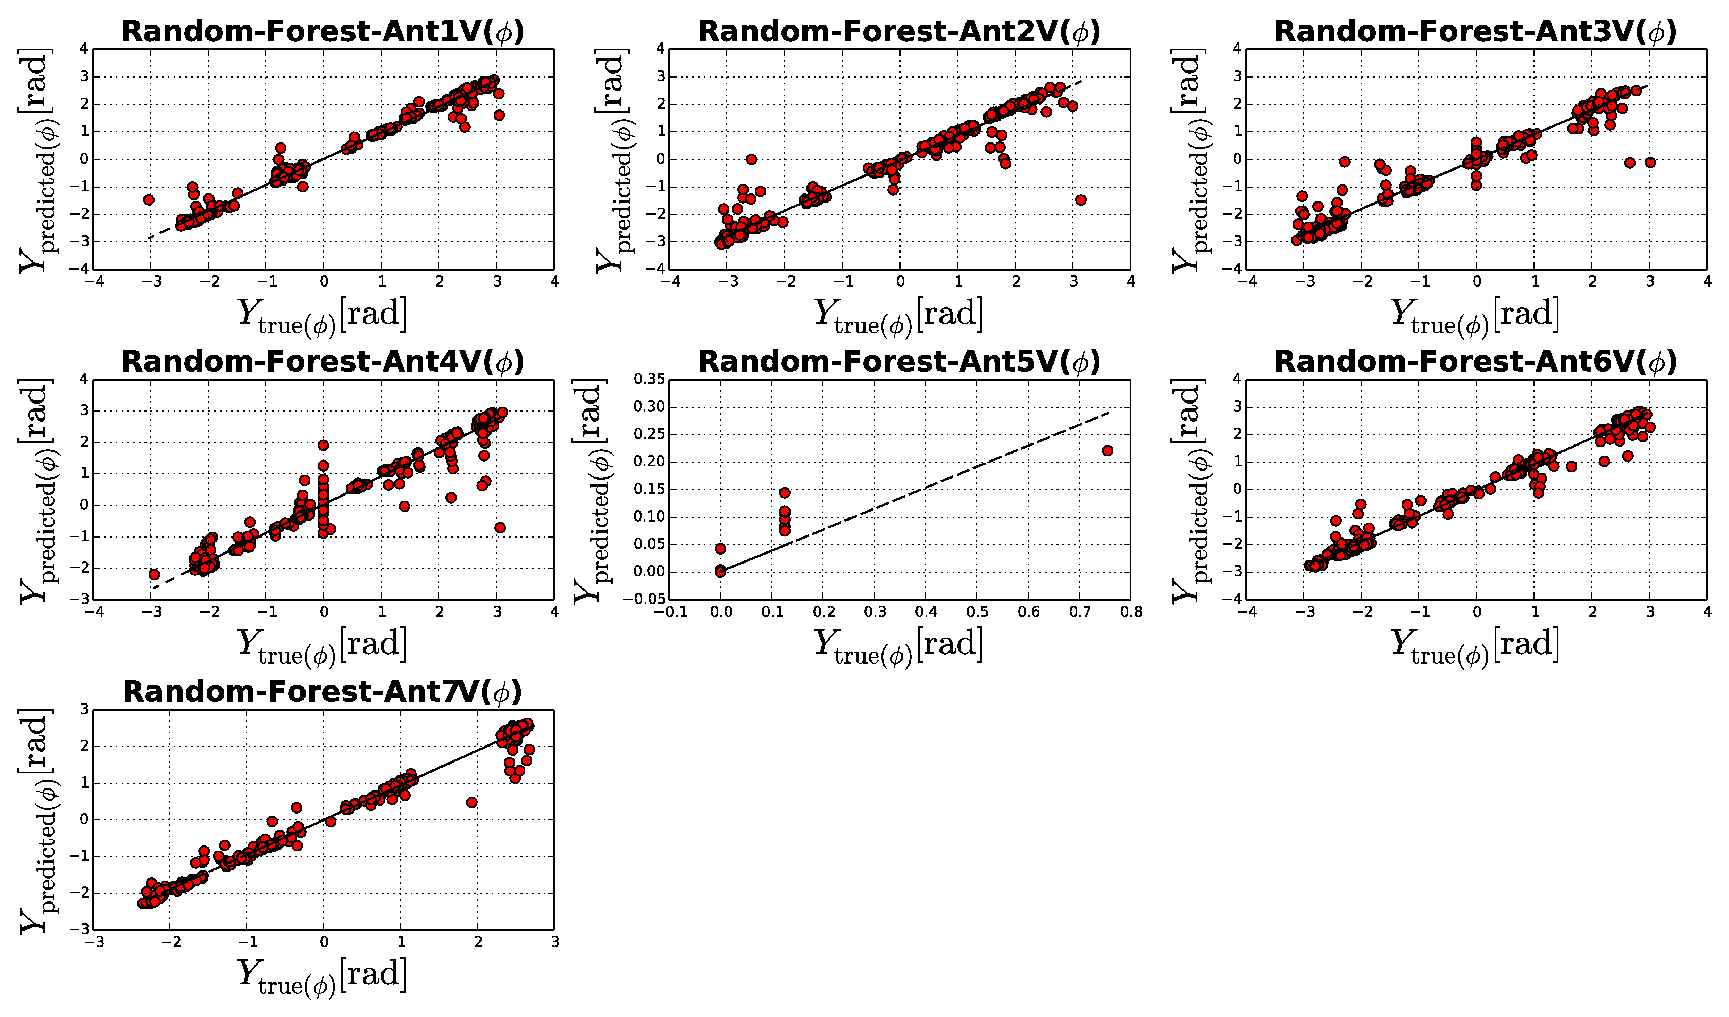
\includegraphics[width=\textwidth]{images/Random-ForestVphase.eps} 
        \caption{Phase gain solutions for V-polarization} \label{A3}
    \end{subfigure}
    
      \begin{subfigure}[t]{0.52\textheight}
       
        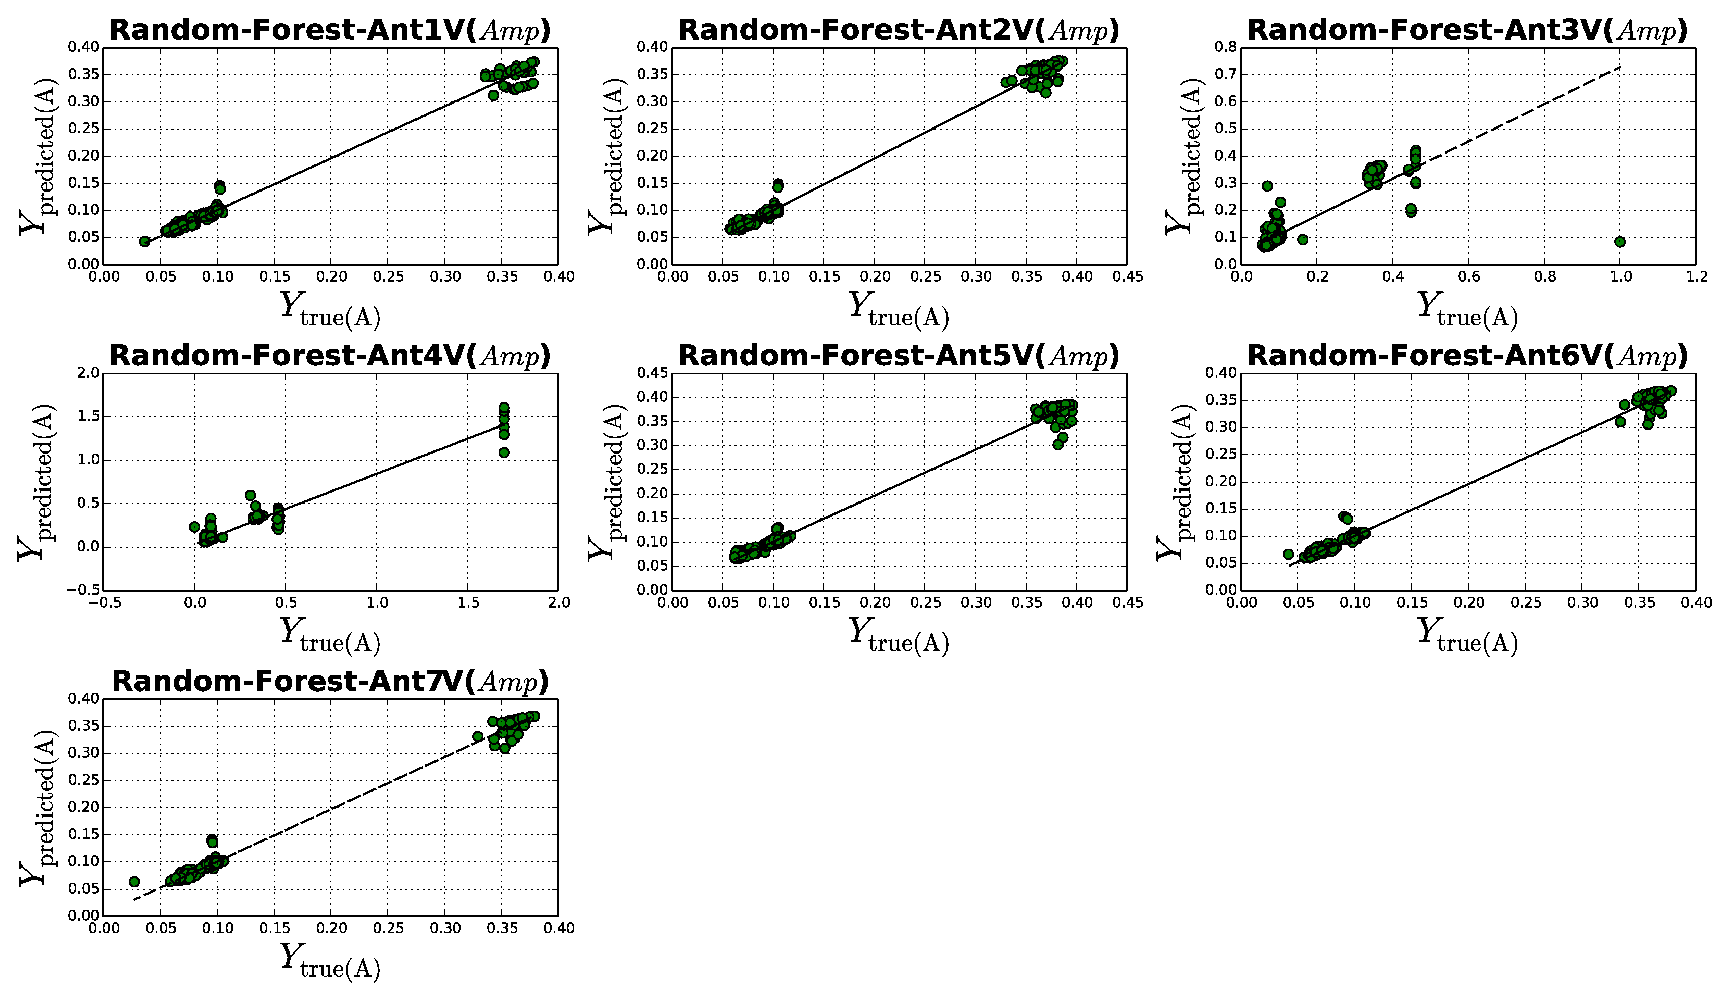
\includegraphics[width=\textwidth]{images/Random-ForestVamp.eps} 
        \caption{Amplitude gain solutions for V-polarization} \label{B3}
    \end{subfigure}
    \caption{Results obtained from the random forest learning algorithm with randomized search optimization algorithm. (\subref{A3}) and (\subref{B3}) are the predicted phase gain solutions $\textbf{Y}_{predicted}$ by the random forest vs the true gain solutions $\textbf{Y}_{true}$ (CASA) for V polarization. We observe that the random forest is performing better in predicting the V-polarization amplitude and phase gain solutions with few outlier points. }
    \label{BBB2}
    \end{figure} 
   
\begin{table}[H]
\begin{center}
\scalebox{0.7}{
\begin{tabular}{| c | c | c | c | c |}
\hline
Antenna & \multicolumn{4}{ c |}{\textbf{Random forest phase}}  \\ 
\cline{2-5}
& Rmse & Rmae & R2score & Explained $\sigma^2$\\
\hline
 Uniform average-H &0.368 & 0.352 & 0.912   & 0.912 \\ 
Uniform average-V &0.256 & 0.311 & 0.939   & 0.939\\ \hline
 & \multicolumn{4}{ c |}{\textbf{Random forest amplitude}}  \\ 
\cline{1-5}
\hline
Uniform average-H &0.028 & 0.087 & 0.918   & 0.919 \\ 
Uniform average-V &0.028 & 0.088 & 0.916    & 0.917\\ \hline

\end{tabular}}
\end{center}
\caption{The table shows the performance of the random forest algorithm in predicting the amplitude and phase  gain solutions for both H and V polarizations as shown in Figures \ref{BB2} and \ref{BBB2}. The values shown represent the uniform average of all KAT-7 antennas, i.e., all output measures are averaged with uniform weight. We observe that most of the predictions stay near the ideal truth values with rmse \ref{MSE} and rmae \ref{MAE}  $\approx <$ 0.5, $R^2$ \ref{R2score} and explained variance $V$ \ref{ExV} converging to 1.}
\end{table}

\subsection{K-nearest neighbor-RUN}
\begin{figure}[H]
   \centering
    \begin{subfigure}[t]{0.52\textheight}
        
        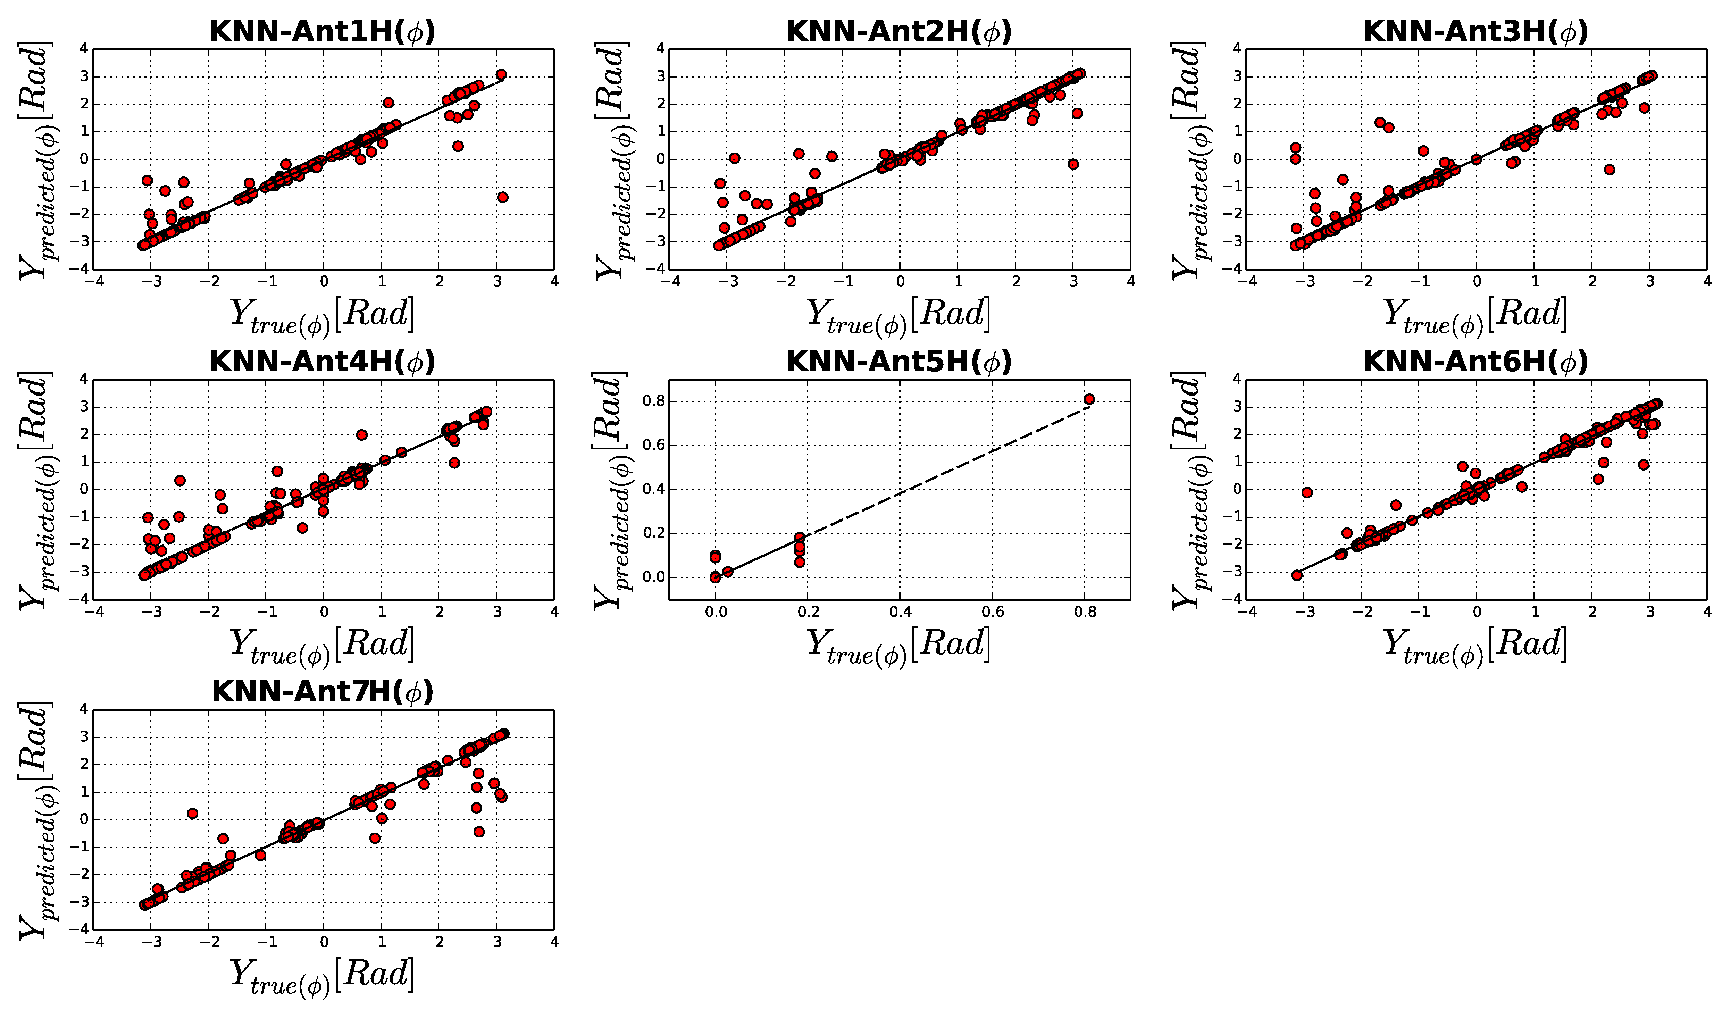
\includegraphics[width=\textwidth]{images/KNNHphase.eps} 
        \caption{Phase gain solutions for H-polarization} \label{A4}
    \end{subfigure}
    
      \begin{subfigure}[t]{0.52\textheight}
       
        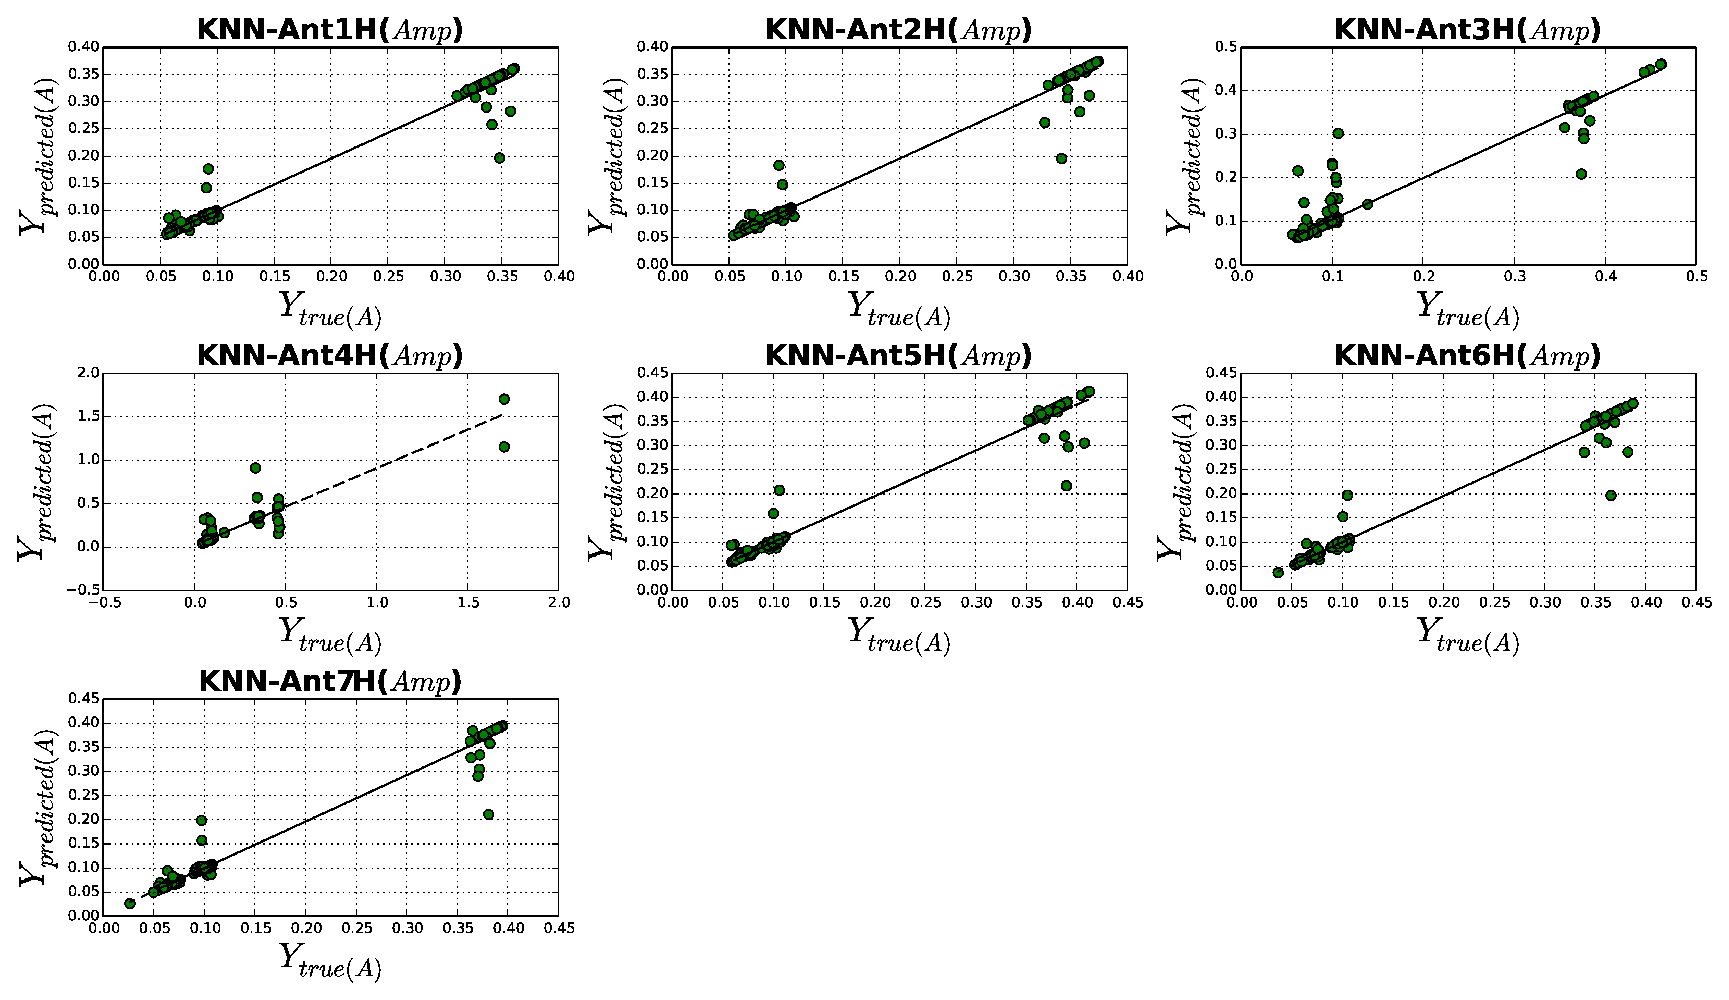
\includegraphics[width=\textwidth]{images/KNNHamp.eps} 
        \caption{Amplitude gain solutions for H-polarization} \label{B4}
    \end{subfigure}
    \caption{Results obtained from the K-nearest neighbor learning algorithm with randomized search optimization algorithm. (\subref{A4}) and (\subref{B4}) are the predicted gain solutions $\textbf{Y}_{predicted}$ by the K-nearest neighbor vs the true gain solutions $\textbf{Y}_{true}$ (CASA) for H-polarization. We observe that the K-nearest neighbor is performing better in predicting the H-polarization amplitude and phase gain solutions with few outlier points.}
    \label{BB4}
    \end{figure}
    
\begin{figure}[H]
   \centering
    \begin{subfigure}[t]{0.52\textheight}
        
        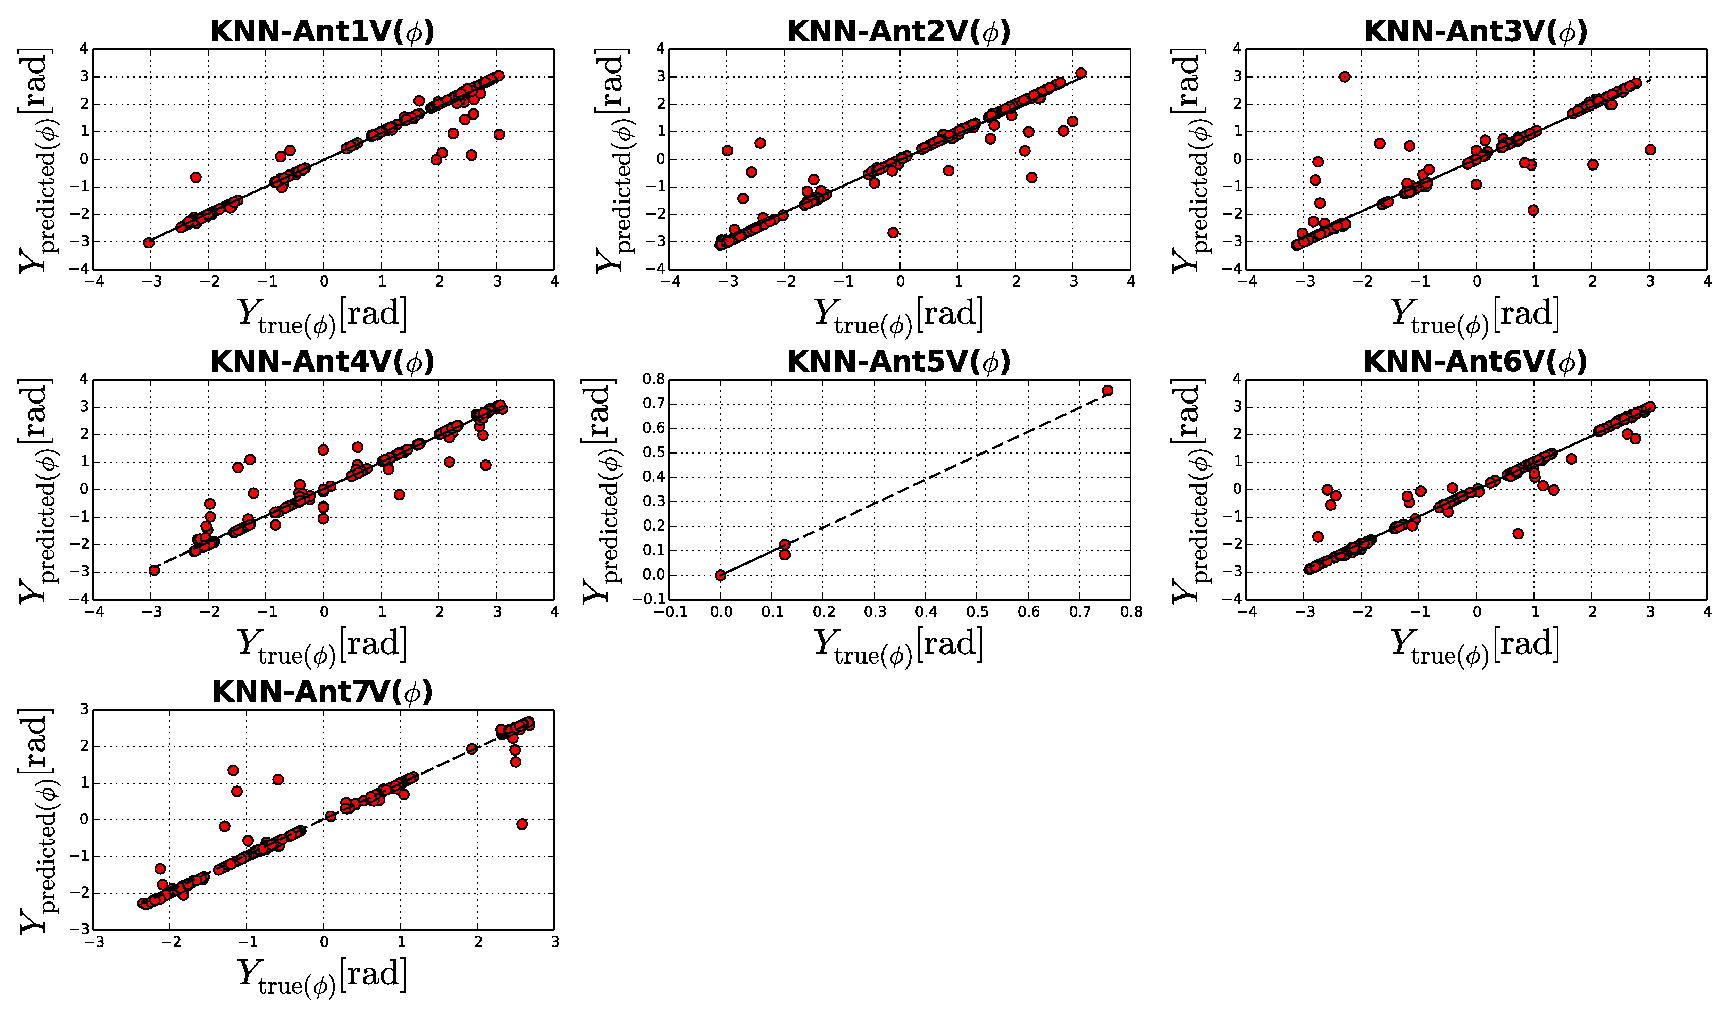
\includegraphics[width=\textwidth]{images/KNNVphase.eps} 
        \caption{Phase gain solutions for V-polarization} \label{A5}
    \end{subfigure}
    
      \begin{subfigure}[t]{0.52\textheight}
       
        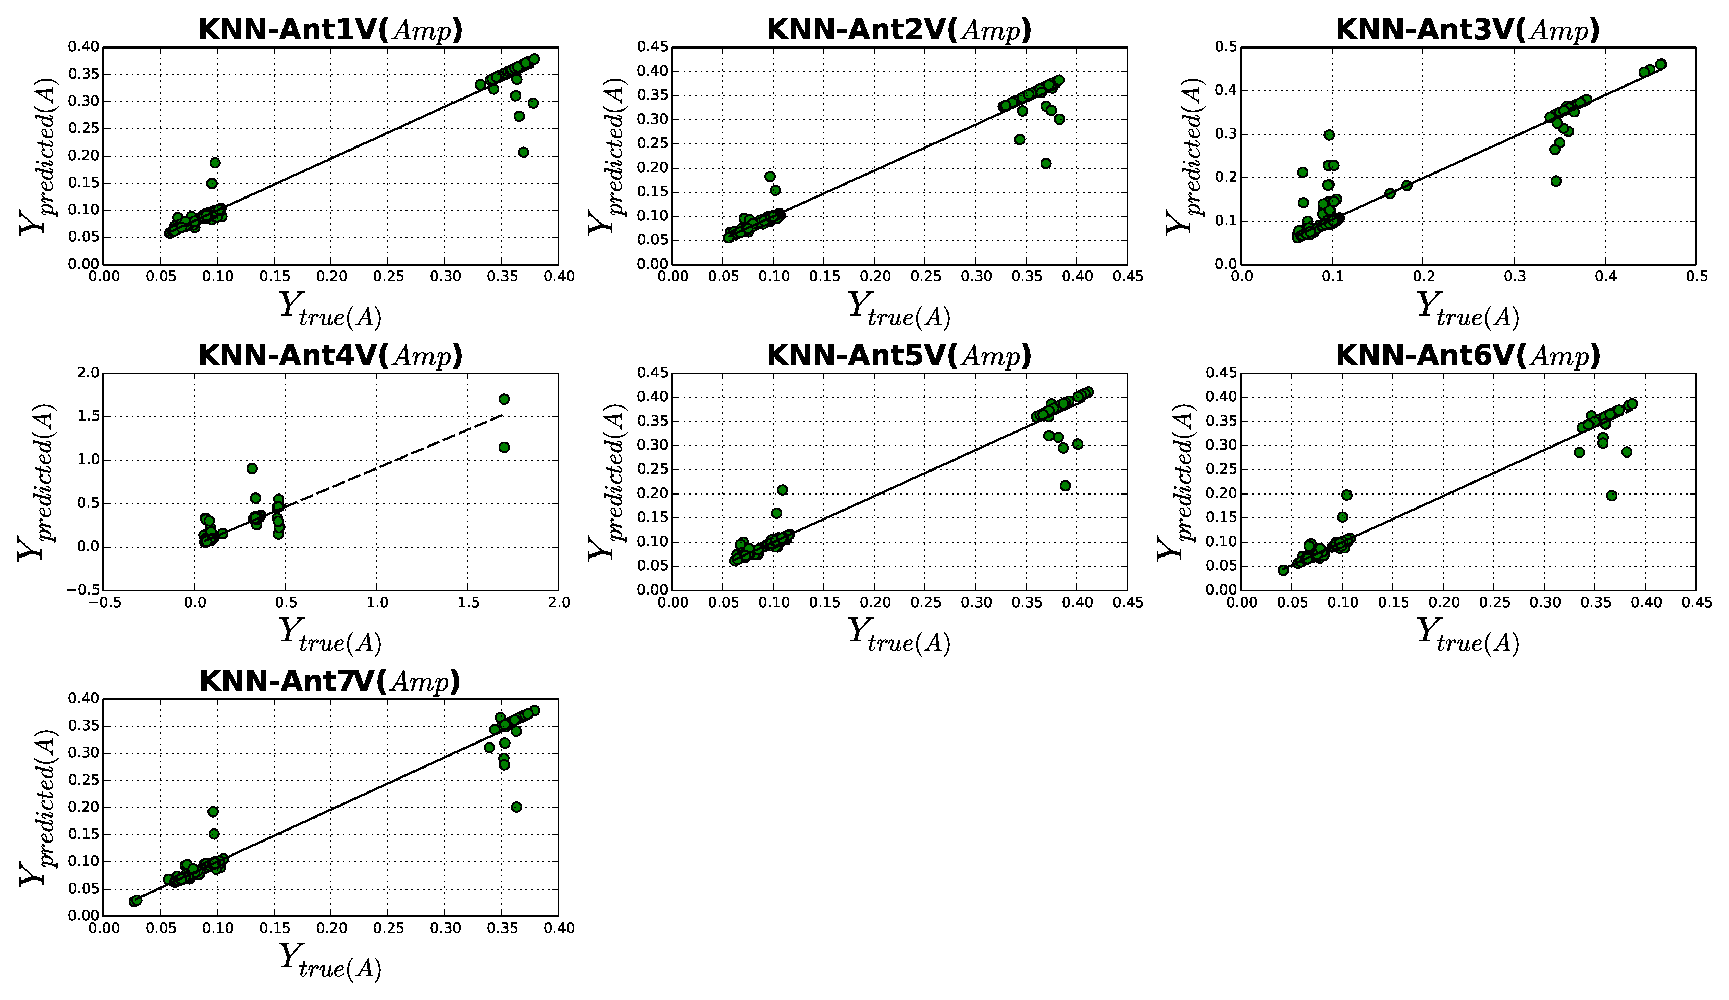
\includegraphics[width=\textwidth]{images/KNNVamp.eps} 
        \caption{Amplitude gain solutions for V-polarization} \label{B5}
    \end{subfigure}
    \caption{Results obtained from the K-nearest neighbor learning algorithm with randomized search optimization algorithm. (\subref{A5}) and (\subref{B5}) are the predicted phase gain solutions $\textbf{Y}_{predicted}$ by the K-nearest neighbor vs the true phase gain solutions $\textbf{Y}_{true}$ (CASA) for V-polarization. We observe that the K-nearest neighbor is performing better in predicting the V-polarization amplitude and phase gain solutions with few outlier points. }
    \label{BBB4}
    \end{figure} 
   

\begin{table}[H]
\label{T:equipos}
\begin{center}
\scalebox{0.7}{
\begin{tabular}{| c | c | c | c | c |}
\hline
Antenna & \multicolumn{4}{ c |}{\textbf{KNN phase}}  \\ 
\cline{2-5}
& Rmse &Rmae &R2score&Explained$\sigma^2$\\
\hline

 Uniform average-H &0.352 & 0.258 & 0.945    & 0.945 \\ 
Uniform average-V &0.291 & 0.239 & 0.961    & 0. 961\\ \hline
 & \multicolumn{4}{ c |}{\textbf{KNN amplitude}}  \\ 
\cline{1-5}
\hline
 Uniform average-H &0.352 & 0.258 & 0.945    & 0.945 \\ 
Uniform average-V &0.291 & 0.239 & 0.961    & 0. 961\\ \hline
\end{tabular}}
\end{center}
\caption{The table shows the performance of the K-nearest neighbor algorithm in predicting the amplitude and phase gain solutions for both H and V polarizations as shown in Figure \ref{BB4} and \ref{BBB4}. The values shown represent the uniform average of all KAT-7 antennas, i.e., all output measures are averaged with uniform weight. Most of the predictions stay near the ideal truth values with RMSE \ref{MSE} and rmae \ref{MAE}  $\approx <$ 0.5, $R^2$ \ref{R2score} and explained variance $V$ \ref{ExV} are converging to 1.}
\end{table}


\subsection{Extremely randomized tree-RUN}

\begin{figure}[H]
   \centering
    \begin{subfigure}[t]{0.52\textheight}
        
        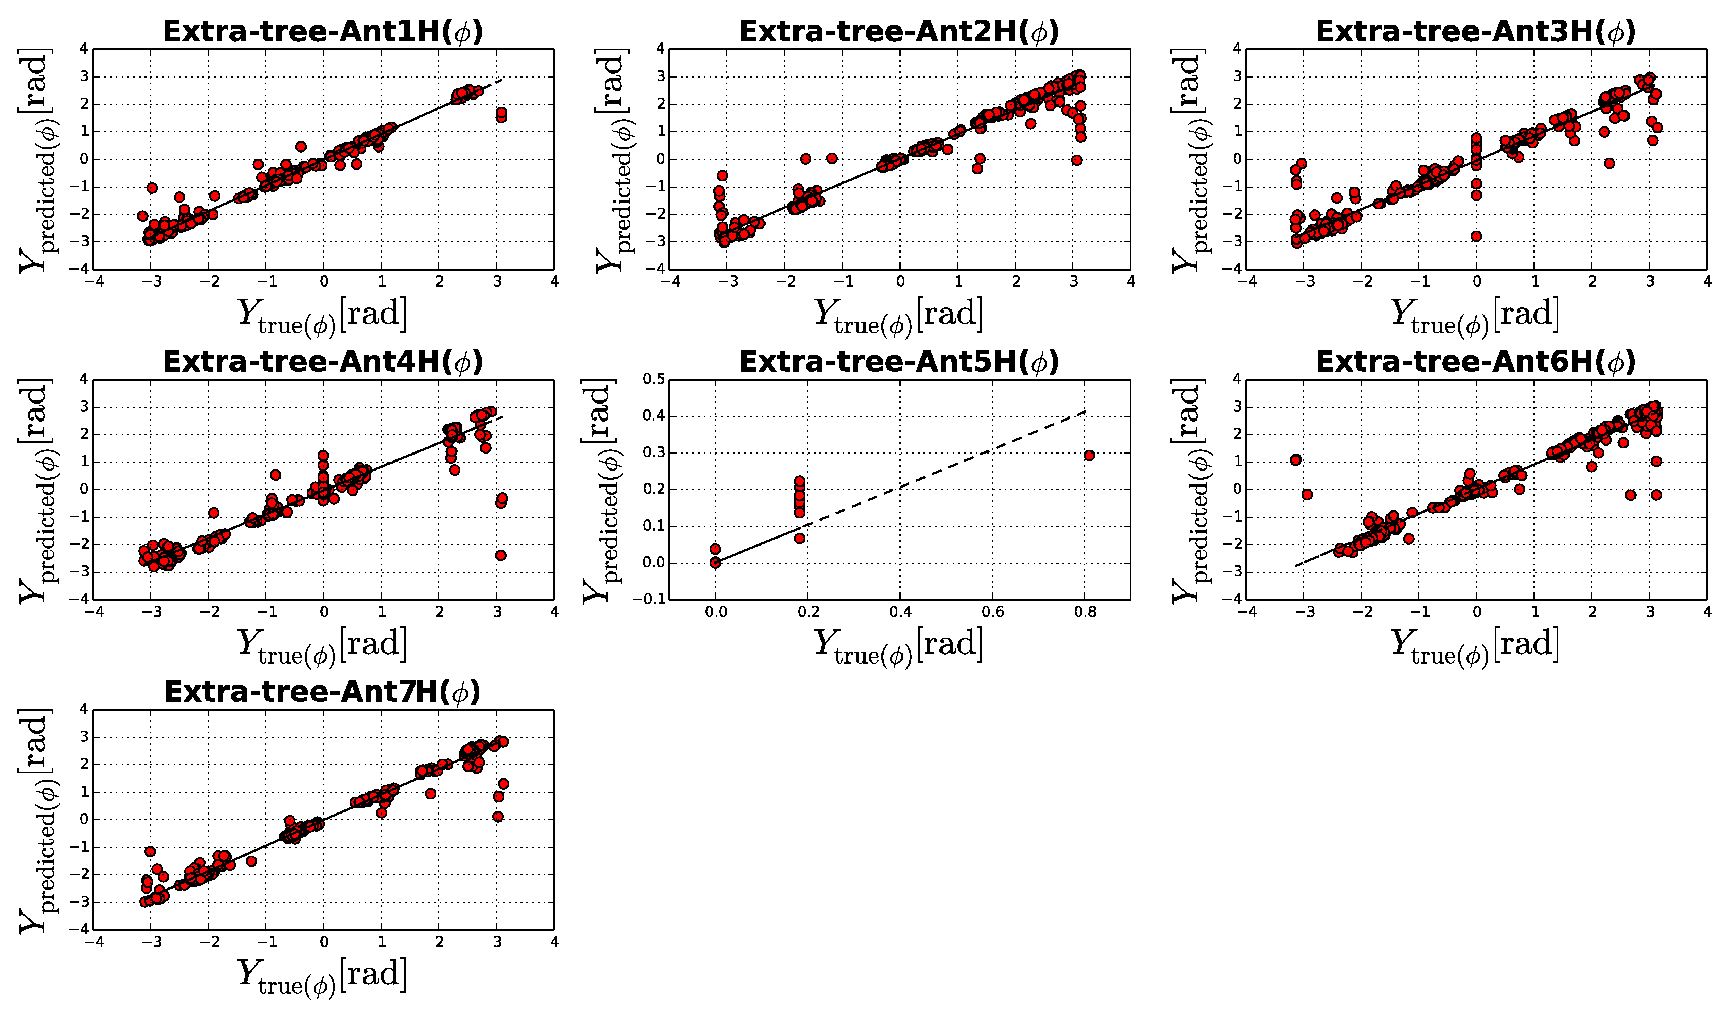
\includegraphics[width=\textwidth]{images/Extra-treeHphase.eps} 
        \caption{Phase gain solutions for H-polarization} \label{A6}
    \end{subfigure}
    
      \begin{subfigure}[t]{0.52\textheight}
       
        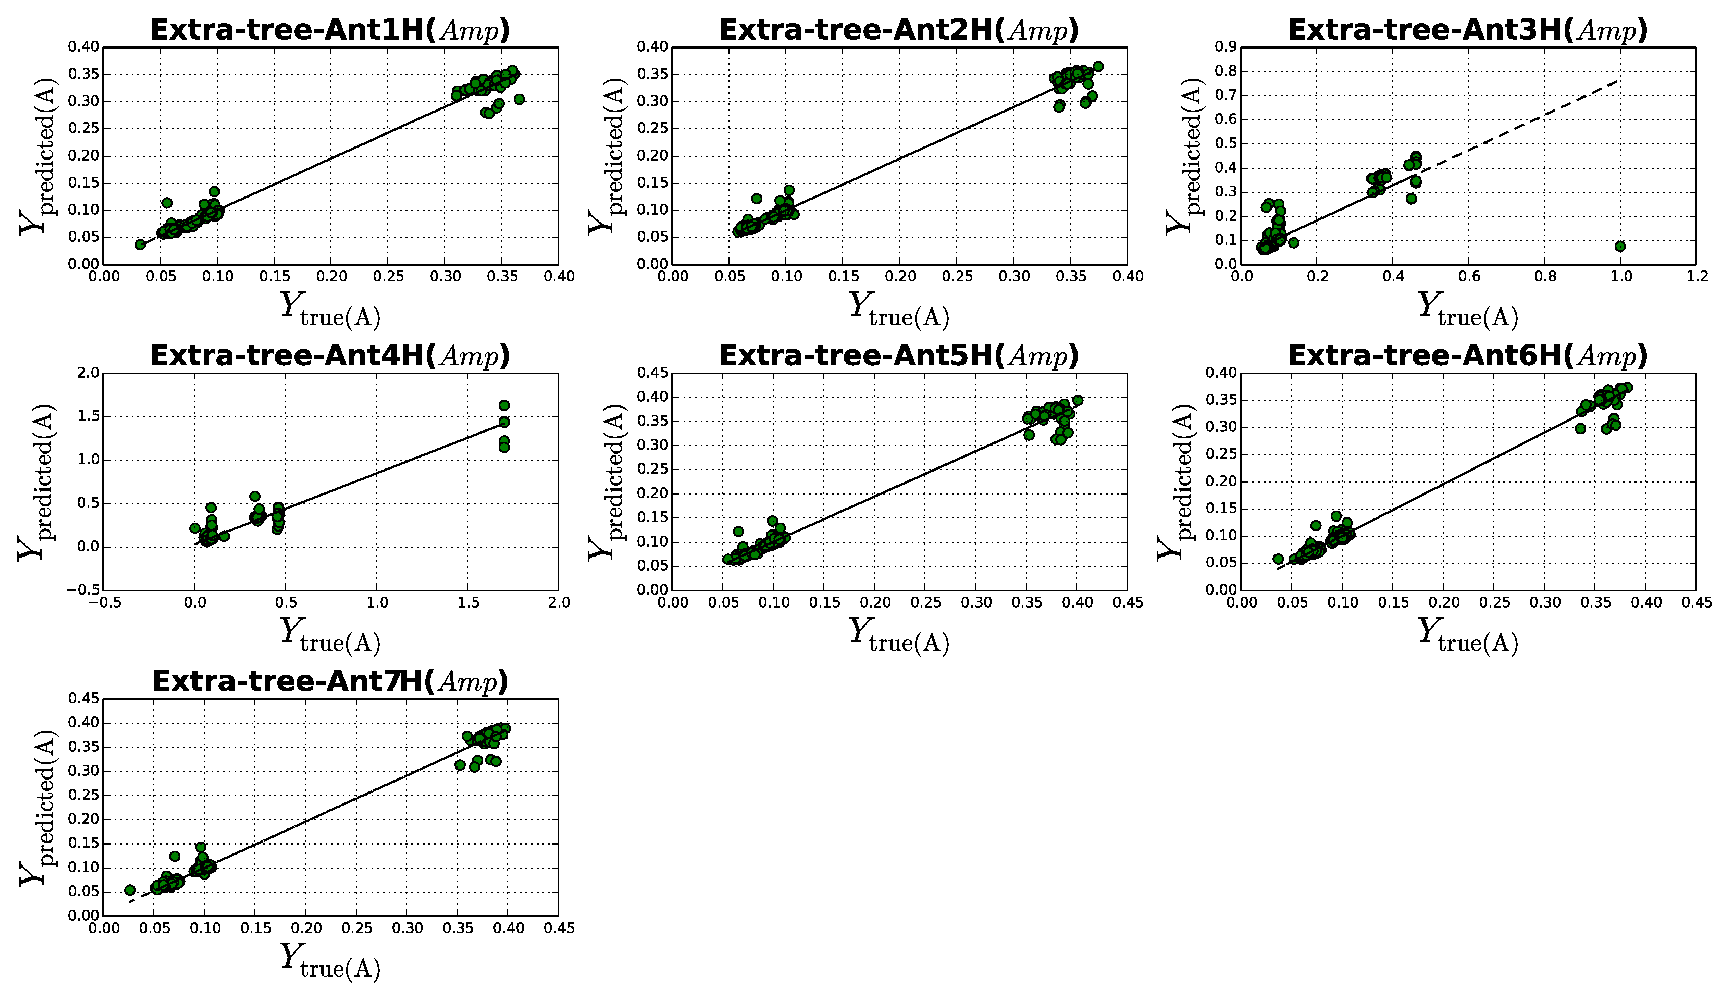
\includegraphics[width=\textwidth]{images/Extra-treeHamp.eps} 
        \caption{Amplitude gain solutions for H-polarization} \label{B6}
    \end{subfigure}
    \caption{Results obtained from the extremely randomized tree learning algorithm with randomized search optimization algorithm. (\subref{A6}) and (\subref{B6}) are the predicted gain solutions $\textbf{Y}_{predicted}$ by the extremely randomized tree  vs the true gain solutions $\textbf{Y}_{true}$ (CASA) for H-polarization. We observe that the extremely randomized tree is performing better in predicting the H-polarization amplitude and phase gain solutions with few outlier points.}
    \label{BB7}
    \end{figure}
    
\begin{figure}[H]
   \centering
    \begin{subfigure}[t]{0.52\textheight}
        
        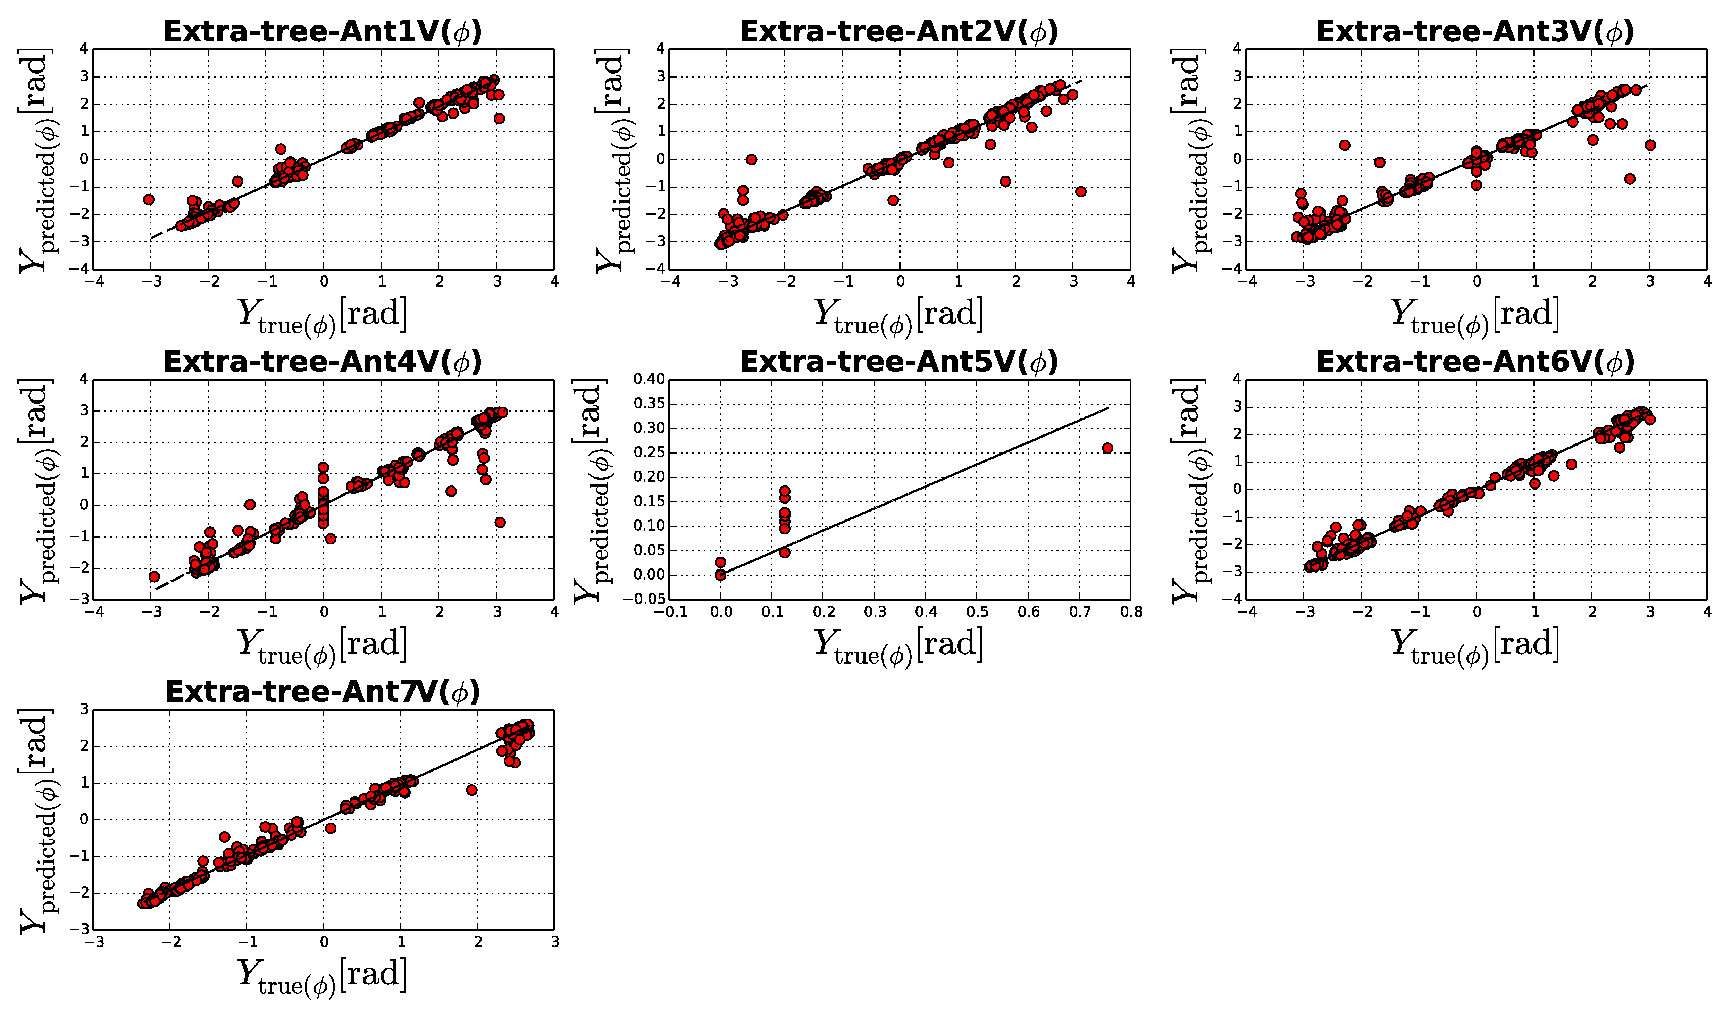
\includegraphics[width=\textwidth]{images/Extra-treeVphase.eps} 
        \caption{Phase gain solutions for V-polarization} \label{A7}
    \end{subfigure}
    
      \begin{subfigure}[t]{0.52\textheight}
       
        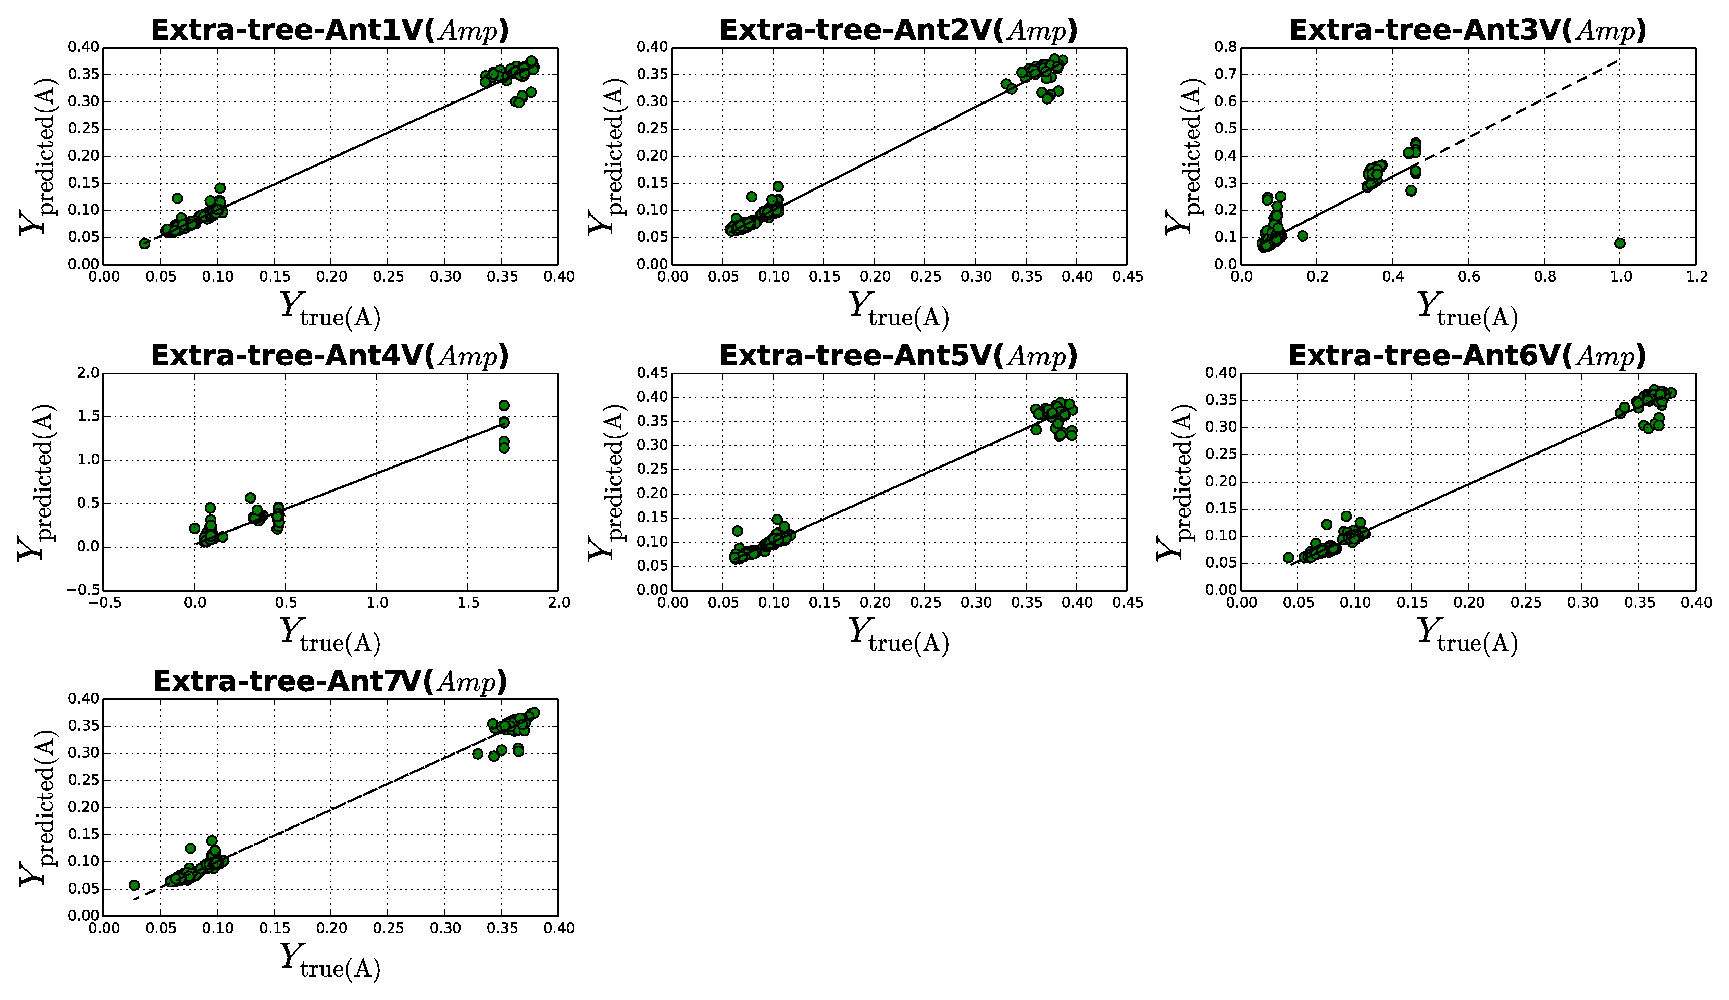
\includegraphics[width=\textwidth]{images/Extra-treeVamp.eps} 
        \caption{Amplitude gain solutions for V-polarization} \label{B7}
    \end{subfigure}
    \caption{Results obtained from the extremely randomized tree learning algorithm with randomized search optimization algorithm. (\subref{A7}) and (\subref{B7}) are the predicted gain solutions $\textbf{Y}_{predicted}$ by the learning algorithm vs the true gain solutions $\textbf{Y}_{true}$ (CASA) for V-polarization. We observe that the extremely randomized tree is performing better in predicting the V-polarization amplitude and phase gain solutions with few outlier points. }
    \label{BBB7}
    \end{figure} 
   
\begin{table}[H]
\label{T:equipos}
\begin{center}
\scalebox{0.7}{
\begin{tabular}{| c | c | c | c | c |}
\hline
Antenna & \multicolumn{4}{ c |}{\textbf{Extremely randomized phase}}  \\ 
\cline{2-5}
& rmse & Rmae & R2score & Explained $\sigma^2$\\
\hline
 Uniform average-H &0.337 & 0.336 & 0.936    & 0.936 \\ 
Uniform average-V &0.235 & 0.301 & 0.956    & 0. 957\\ \hline
 & \multicolumn{4}{ c |}{\textbf{Extremely randomized tree  amplitude}}  \\ 
\cline{1-5}
\hline
Uniform average-H &0.027 & 0.083 & 0.925    & 0.925 \\ 
Uniform average-V &0.027 & 0.083 & 0.923    & 0.923 \\ \hline
\end{tabular}}
\end{center}
\caption{The table shows the performance of the extremely randomized tree algorithm in predicting the amplitude and phase gain solutions for both H and V polarizations as shown in figures \ref{BB7} and \ref{BBB7}. The values shown represents the uniform average of all KAT-7 antennas, i.e., all output measures are averaged with uniform weight. Most of the predictions stay near the ideal truth values with rmse \ref{MSE} and rmae \ref{MAE}  $\approx <$ 0.5, $R^2$ \ref{R2score} and explained variance $V$ \ref{ExV} are converging to 1.}
\end{table}

\subsection{Summary of results}

This section report the accuracy measure obtained for each learning algorithm when evaluating on testing dataset. In every model there are four plots, each for amplitude and phase H $\&$ V-polarization. The $y-axis$ in each subplot is the predicted gain amplitude and phase solutions using the testing sensor data, and the $x-axis$ is the ground truth amplitude and phase gain solution. Note that the two-cluster grouping of points in the predicted vs ground truth amplitude plots in Figures \ref{B1}, \ref{B2}, \ref{B3}, \ref{B4}, \ref{B5}, \ref{B6}, \ref{B7} are due to the sinusoidal variation of the amplitude gain solutions as shown in Figure \ref{amp}. We tested our models using using the appropriate regression evaluation methods: RMSE, RMAE, r2score and the explained variance. The evaluation results obtained from the extremely randomized trees, random forest, and K-nearest neighbor are accurate with H-polarization RMSE of $\approx 0.3$  and V-polarization of $\approx 0.2$ for phase gain solution prediction as shown in Figures \ref{A2}, \ref{A3}, \ref{A4}, \ref{A5}, \ref{A6}, \ref{A7}, \ref{A7}. We observe that the amplitude gain solution prediction has better accuracy for random forest and extremely randomized tree on H $\&$ V polarization with RMSE error being $\approx 0.02$, much less than the phase gain solution prediction, as shown in Figures \ref{B2}, \ref{B3}, \ref{B6}, \ref{B7}. We further observe that most of the predictions stay near the ground truth values with a coefficient of determination $R^2$ score converging to 1 for Random forest, extremely randomized trees and K-nearest neighbors with few outlying points that can be due to errors in calibration solution generation and radio frequency interference. On the other we observe that the decision tree algorithm is performing in predicting the amplitude and phase gain solutions for H and V polarization. This is likely due to overfitting of the model. 


 %When fitting a straight line(slope) between the predicted and the true we  observe there is only few outlying points.
\subsection{Testing on new dataset}

Once one is satisfied with the performance of the learning algorithms in predicting the calibration solutions accurately from the testing dataset, in this section new sensor data extracted from new (unseen) KAT-7 observations with the phase calibrator source PKS1623-586 can be used to predict the calibration solutions. This process is called model validation. Since the model was trained on normalized data, one first normalizes the new sensor data with mean $\mu$ and standard deviation $\sigma$ obtained from the normalization of the training dataset.
\begin{align}
\text{scaled-sensor data}= \frac{\text{sensor data}- \mu}{\sigma}
\end{align}

One makes use of a three-observation dataset to perform the unbiased evaluation of the final model fit. These are a subset of the Circinus X-1 KAT-7 commissioning observations taken from December 2011 - June 2012. In each validation dataset, one compares the performance of decision tree, random forest, K-nearest neighbor and extremely randomized trees. One compares these results with gain amplitude and phase calibration solutions obtained from CASA 1GC for H $\&$ V-polarization. 

%\subsubsection{Observation test-1}
%In this section, the plot results obtained from the validation dataset-1 vs CASA solutions. From dataset-1, one observes that the decision tree perfectly predicts the gain phase calibration solutions similar to CASA in Figure \ref{obs1} better than the other models in Figures \ref{obs2}, \ref{obs3}, \ref{obs4}. In the gain amplitude prediction one observes that only random forest and extremely randomized trees perform better, as shown in Figures \ref{ra1} and \ref{ea1}. 
%
% \begin{figure}[H]
%    \includegraphics[ height=13cm, width=16cm]{images/Phasegain.eps}
%    \caption{This figure shows the response of the decision tree learning algorithm in predicting the phase gain solutions for the calibrator PKS1613-586 from the validation dataset-1. In each subplot the CASA calculated phase gain solutions for H (blue) and V (green) polarization vs the learning algorithm (ZCal) predicted phase gain solutions for H (red) and V (yellow) polarization as shown.}
%    \label{obs1}
%\end{figure}
%
%\begin{figure}[H]
%    \includegraphics[ height=13cm, width=16cm]{images/DCampgain.eps}
%    \caption{This figure shows the response of the decision tree learning algorithm in predicting the amplitude gain solutions for the calibrator PKS1613-586 from the validation dataset-1. In each subplot the CASA calculated amplitude gain solutions for H (blue) and V (green) polarization vs the learning algorithm (ZCal) predicted amplitude gain solutions for H (red) and V (yellow) polarization as shown.}
%     \label{da1}
%\end{figure}
%
%
%\begin{figure}[H]
%    \includegraphics[ height=13cm, width=16cm]{images/RFphasegain.eps}
%    \caption{This figure shows the response of the random forest learning algorithm in predicting the phase gain solutions for the calibrator PKS1613-586 from the validation dataset-1. In each subplot the CASA calculated phase gain solutions for H (blue) and V (green) polarization vs the learning algorithm (ZCal) predicted phase gain solutions for H (red) and V (yellow) polarization as shown.}
%    \label{obs2}
%\end{figure}
%
%\begin{figure}[H]
%    \includegraphics[ height=13cm, width=16cm]{images/RFampegain.eps}
%    \caption{This figure shows the response of the random forest learning algorithm in predicting the amplitude gain solutions for the calibrator PKS1613-586 from the validation dataset-1. In each subplot the CASA calculated amplitude gain solutions for H (blue) and V (green) polarization vs the learning algorithm (ZCal) predicted amplitude gain solutions for H (red) and V (yellow) polarization as shown.}
%     \label{ra1}
%\end{figure}
%
%\begin{figure}[H]
%    \includegraphics[ height=13cm, width=16cm]{images/KNNPhasegain.eps}
%    \caption{This figure shows the response of the K-nearest neighbor learning algorithm in predicting the phase gain solutions for the calibrator PKS1613-586 from the validation dataset-1. In each subplot the CASA calculated phase gain solutions for H (blue) and V (green) polarization vs the learning algorithm (ZCal) predicted phase gain solutions for H (red) and V (yellow) polarization as shown.}
%    \label{obs3}
%\end{figure}
%
%\begin{figure}[H]
%    \includegraphics[ height=13cm, width=16cm]{images/KNNampgain.eps}
%    \caption{This figure shows the response of the K-nearest neighbor learning algorithm in predicting the amplitude gain solutions for the calibrator PKS1613-586 from the validation dataset-1. In each subplot the CASA calculated amplitude gain solutions for H (blue) and V (green) polarization vs the learning algorithm (ZCal) predicted amplitude gain solutions for H (red) and V (yellow) polarization as shown.}
%     \label{ka1}
%\end{figure}
%
%\begin{figure}[H]
%    \includegraphics[ height=13cm, width=16cm]{images/EXTPhasegain.eps}
%    \caption{This figure shows the response of the extremely randomized tree learning algorithm in predicting the phase gain solutions for the calibrator PKS1613-586 from the validation dataset-1. In each subplot the CASA calculated phase gain solutions for H (blue) and V (green) polarization vs the learning algorithm (ZCal) predicted phase gain solutions for H (red) and V (yellow) polarization as shown.}
%    \label{obs4}
%\end{figure}
%
%\begin{figure}[H]
%    \includegraphics[ height=13cm, width=16cm]{images/EXTampgain.eps}
%    \caption{This figure shows the response of the extremely randomized tree learning algorithm in predicting the amplitude gain solutions for the calibrator PKS1613-586 from the validation dataset-1. In each subplot the CASA calculated amplitude gain solutions for H (blue) and V (green) polarization vs the learning algorithm (ZCal) predicted amplitude gain solutions for H (red) and V (yellow) polarization as shown.}
%     \label{ea1}
%\end{figure}

\subsubsection{Observation test-1}
This section gives the plot results obtained from the validation observation.  Each plot shows the gain calibration solutions predicted by the models: decision tree, random forest, K-nearest neghbors and extremely randomised trees using the new observation's sensor data. We compare the predicted gain calibration solutions with 1GC CASA generated solutions to validate each model's performance. 

\begin{figure}[H]
    \includegraphics[ height=13cm, width=16cm]{images/DCPhasegain1015.eps}
    \caption{This figure shows the response of the decision tree learning algorithm in predicting the H $\&$ V phase gain solutions for the calibrator PKS1613-586 from the validation dataset-1. In each subplot we compare the predicted phase gain solutions (where H polarization is represented by red and V-polarization is represented by yellow) with the CASA generated phase gain solutions (where H polarization is represented by blue and V-polarization is represented by green). The decision tree algorithm is failing to predict the gain phase solutions on the new observation dataset-1.}
    \label{obs5}
\end{figure}

\begin{figure}[H]
    \includegraphics[ height=13cm, width=16cm]{images/DCampgain1015.eps}
    \caption{This figure shows the response of the decision tree learning algorithm in predicting the amplitude gain solutions for the calibrator PKS1613-586 from the validation dataset-1. In each subplot we compare the the predicted amplitude gain solutions (where H polarization is represented by red and V-polarization is represented by yellow) with the CASA generated phase gain solutions (where H polarization is represented by blue and V-polarization is represented by green). The decision tree algorithm is failing to predict the gain amplitude solutions on the new observation dataset-1.}
     \label{da2}
\end{figure}


\begin{figure}[H]
    \includegraphics[ height=13cm, width=16cm]{images/RFPhasegain1015.eps}
    \caption{This figure shows the response of the random forest learning algorithm in predicting the phase gain solutions for the calibrator PKS1613-586 from the validation dataset-1. In each subplot we compare the predicted phase gain solutions (where H polarization is represented by red and V-polarization is represented by yellow) with the CASA generated phase gain solutions (where H polarization is represented by blue and V-polarization is represented by green). The random forest algorithm is failing to predict the gain phase solutions for some antennas and performing well in others with few outliers.}
    \label{obs6}
\end{figure}

\begin{figure}[H]
    \includegraphics[ height=13cm, width=16cm]{images/RFampgain1015.eps}
    \caption{This figure shows the response of the random forest learning algorithm in predicting the amplitude gain solutions for the calibrator PKS1613-586 from the validation dataset-1. In each subplot we compare the predicted amplitude gain solutions (where H polarization is represented by red and V-polarization is represented by yellow) with the CASA generated phase gain solutions (where H polarization is represented by blue and V-polarization is represented by green). The random forest algorithm is failing to predict the gain amplitude solutions in all the antennas, for solutions at time index $<$ 70. We further observe that at time index $80$ the algorithm performing better in predicting the amplitude solutions, slightly close to CASA on the new observation dataset-1.}
     \label{ra2}
\end{figure}

\begin{figure}[H]
    \includegraphics[ height=13cm, width=16cm]{images/KNNPhasegain1015.eps}
    \caption{This figure shows the response of the K-nearest neighbor learning algorithm in predicting the phase gain solutions for the calibrator PKS1613-586 from the validation dataset-1. In each subplot we compare the predicted phase gain solutions (where H polarization is represented by red and V-polarization is represented by yellow) with the CASA generated phase gain solutions (where H polarization is represented by blue and V-polarization is represented by green). The K-nearest neighbor algorithm is failing to predict the gain phase solutions on the new observation dataset-1.}
    \label{obs7}
\end{figure}

\begin{figure}[H]
    \includegraphics[ height=13cm, width=16cm]{images/KNNampgain1015.eps}
    \caption{This figure shows the response of the K-nearest neighbor learning algorithm in predicting the amplitude gain solutions for the calibrator PKS1613-586 from the validation dataset-1. In each subplot we compare the predicted amplitude gain solutions (where H polarization is represented by red and V-polarization is represented by yellow) with the CASA generated phase gain solutions (where H polarization is represented by blue and V-polarization is represented by green). The K-nearest neighbor algorithm is predicting the gain amplitude solutions in all the antennas with a weak match when compared to CASA on the new observation dataset-1.}
     \label{ka2}
\end{figure}

\begin{figure}[H]
    \includegraphics[ height=13cm, width=16cm]{images/EXTPhasegain1015.eps}
    \caption{This figure shows the response of the extremely randomized tree learning algorithm in predicting the phase gain solutions for the calibrator PKS1613-586 from the validation dataset-1. In each subplot we compare the predicted phase gain solutions (where H polarization is represented by red and V-polarization is represented by yellow) with the CASA generated phase gain solutions (where H polarization is represented by blue and V-polarization is represented by green). The extremely randomized tree algorithm is failing to predict the gain phase solutions for some antennas and performing well in others with few outliers.}
    \label{obs8}
\end{figure}

\begin{figure}[H]
    \includegraphics[ height=13cm, width=16cm]{images/EXTampgain1015.eps}
    \caption{This figure shows the response of the extremely randomized tree learning algorithm in predicting the amplitude gain solutions for the calibrator PKS1613-586 from the validation dataset-1. In each subplot we compare the predicted amplitude gain solutions (where H polarization is represented by red and V-polarization is represented by yellow) with the CASA generated phase gain solutions (where H polarization is represented by blue and V-polarization is represented by green). The extremely randomized tree algorithm is failing to predict the gain amplitude solutions in all the antennas, for solutions at time index $<$ 70. We further observe that at time index $80$ the algorithm performing better in predicting the amplitude solutions, slightly close to CASA on the new observation dataset-1.}
     \label{ea2}
\end{figure}

For dataset-1, one observes that the random forest, extremely randomized trees and the K-nearest neighbors have not fully learned to generalise in predicting the gain amplitude calibration solutions than phase. We observe that these model's predictions fail in some part of the samples and successfully predict  well in other. However, the extremely randomized trees algorithm is performing better than the rest as shown in Figure \ref{obs8} and \ref{ea2}.

\subsubsection{Observation test-2}
In this section, the plot results obtained from the validation dataset-2 vs 1GC CASA solutions are given. 


\begin{figure}[H]
    \includegraphics[ height=13cm, width=16cm]{images/DCPhasegain773.eps}
    \caption{This figure shows the response of the decision tree learning algorithm in predicting the H $\&$ V phase gain solutions for the calibrator PKS1613-586 from the validation dataset-2. In each subplot we compare the predicted phase gain solutions (where H polarization is represented by red and V-polarization is represented by yellow) with the CASA generated phase gain solutions (where H polarization is represented by blue and V-polarization is represented by green). The decision tree algorithm is failing to predict the gain phase solutions for some antennas and performing well in others as seen for example in antenna 1 where CASA estimated solutions at 150 $\deg$ and the decision tree at -150 $\deg$ with no outliers. We also observe a successful prediction of antenna 5.}
    \label{obs9}
\end{figure}

\begin{figure}[H]
    \includegraphics[ height=13cm, width=16cm]{images/DCampgain773.eps}
    \caption{This figure shows the response of the decision tree learning algorithm in predicting the amplitude gain solutions for the calibrator PKS1613-586 from the validation dataset-2. In each subplot we compare the the predicted amplitude gain solutions (where H polarization is represented by red and V-polarization is represented by yellow) with the CASA generated phase gain solutions (where H polarization is represented by blue and V-polarization is represented by green). The decision tree algorithm is failing to predict the gain amplitude solutions on the new observation dataset-2. We also observe that it has not learn the sinusoidal behaviour of the amplitude solutions.}
     \label{da3}
\end{figure}


\begin{figure}[H]
    \includegraphics[ height=13cm, width=16cm]{images/RFPhasegain773.eps}
    \caption{This figure shows the response of the random forest learning algorithm in predicting the H $\&$ V phase gain solutions for the calibrator PKS1613-586 from the validation dataset-2. In each subplot we compare the predicted phase gain solutions (where H polarization is represented by red and V-polarization is represented by yellow) with the CASA generated phase gain solutions (where H polarization is represented by blue and V-polarization is represented by green). The random forest algorithm is failing to predict the gain phase solutions for some antennas and slightly performing well in others as seen for example in antenna 1H where CASA estimated solutions at 150 $\deg$ and the random forest at -150 $\deg$. We also observe a successful prediction of antenna 5 solutions.}
    \label{obs10}
\end{figure}

\begin{figure}[H]
    \includegraphics[ height=13cm, width=16cm]{images/RFampgain773.eps}
    \caption{This figure shows the response of the random forest learning algorithm in predicting the amplitude gain solutions for the calibrator PKS1613-586 from the validation dataset-2. In each subplot we compare the the predicted amplitude gain solutions (where H polarization is represented by red and V-polarization is represented by yellow) with the CASA generated phase gain solutions (where H polarization is represented by blue and V-polarization is represented by green). The random forest algorithm is failing to predict the gain amplitude solutions on the new observation dataset-2.}
     \label{ra3}
\end{figure}

\begin{figure}[H]
    \includegraphics[ height=13cm, width=16cm]{images/KNNPhasegain773.eps}
    \caption{This figure shows the response of the K-nearest neighbor learning algorithm in predicting the H $\&$ V phase gain solutions for the calibrator PKS1613-586 from the validation dataset-2. In each subplot we compare the predicted phase gain solutions (where H polarization is represented by red and V-polarization is represented by yellow) with the CASA generated phase gain solutions (where H polarization is represented by blue and V-polarization is represented by green). The K-nearest neighbor algorithm is failing to predict the gain phase solutions, except for antenna 5 which was used as a reference antenna.}
    \label{obs11}
\end{figure}

\begin{figure}[H]
    \includegraphics[ height=13cm, width=16cm]{images/KNNampgain773.eps}
    \caption{This figure shows the response of the K-nearest neighbor learning algorithm in predicting the amplitude gain solutions for the calibrator PKS1613-586 from the validation dataset-2. In each subplot we compare the the predicted amplitude gain solutions (where H polarization is represented by red and V-polarization is represented by yellow) with the CASA generated phase gain solutions (where H polarization is represented by blue and V-polarization is represented by green). The K-nearest neighbor algorithm is failing to predict the gain amplitude solutions on the new observation dataset-2. We observe that at time index > 12 the algorithm is predicting solutions slightly  closer to what CASA estimated with few outliers for antenna 1,2,3,5, 6 and 7.}
     \label{ka3}
\end{figure}

\begin{figure}[H]
    \includegraphics[ height=13cm, width=16cm]{images/EXTPhasegain773.eps}
    \caption{This figure shows the response of the extremely randomized tree learning algorithm in predicting the H $\&$ V phase gain solutions for the calibrator PKS1613-586 from the validation dataset-2. In each subplot we compare the predicted phase gain solutions (where H polarization is represented by red and V-polarization is represented by yellow) with the CASA generated phase gain solutions (where H polarization is represented by blue and V-polarization is represented by green). The extremely randomized tree algorithm is failing to predict the gain phase solutions for some antennas and slightly performing well in others as seen for example in antenna 1H where CASA estimated solutions at 150 $\deg$ and the extremely randomized tree at -150 $\deg$. We also observe a successful prediction of antenna 5 solutions.}
    \label{obs12}
\end{figure}

\begin{figure}[H]
    \includegraphics[ height=13cm, width=16cm]{images/EXTampgain773.eps}
    \caption{This figure shows the response of the extremely randomized tree learning algorithm in predicting the amplitude gain solutions for the calibrator PKS1613-586 from the validation dataset-2. In each subplot we compare the the predicted amplitude gain solutions (where H polarization is represented by red and V-polarization is represented by yellow) with the CASA generated phase gain solutions (where H polarization is represented by blue and V-polarization is represented by green). The extremely randomized tree algorithm is failing to predict the gain amplitude solutions on the new observation dataset-2.}
     \label{ea3}
\end{figure}

For dataset-2, one observe that the random forest, extremely randomized trees, K-nearest neighbors and decision tree algorithm have not learned to generalise in predicting the gain amplitude and phase solutions when compared with CASA. Unlike from the observation dataset-1, there isn’t no match with CASA in all the models and data samples. 







 % You do not need to have exactly 4 chapters.
                 % It is probably a good minimum, with 5 chapters 
                 % average, and 7 chapters might be a maximum.
\chapter{Behaviour analysis of antennas}
In this Chapter we analyse and discuss each antenna behaviour looking at the results obtained in predicting the gain solutions from each experiment of our learning algorithms for both polarization H in Section \ref{Hp} and V polarization in Section \ref{Vp}. 

\section{Pointing sensor distribution}
\begin{figure}[H]
    \includegraphics[ height=12cm, width=16cm]{images/Distribution.eps}
    \caption{This figure is showing the distribution of the averaged pointing data per antenna during the tracking of the calibrator source PKS1613-586. The blue line is the average pointing per antenna, and the red line is the reference probability distribution for all the antennas.}
    \label{Point}
\end{figure}
The Figure \ref{Point} illustrate how the pointing sensor data per antenna are distributed. This gives us details about whether or not the antennas were pointing at the same position. We observe that Each antenna pointing is distributed differently from the reference probability distribution. These small offsets might have contribution in prediction errors of amplitude and phase gain solutions.

\section{H-polarization amplitude and phase}
\label{Hp}
As seen in Figure \ref{phase}, the gain phase solutions obtained from CASA for antenna 5 is zero. This is due to the selection of antenna 5 as a reference antenna during the calibration of G solutions. Fundamentally, the baseline visibility phases measured by an interferometry are exclusively different between antennas, and so no absolute phase reference exists \citep{taylor1999synthesis}. Antenna-based calibration solutions thus have phases which are constrained only to satisfy the observed visibility phases; further, each solution in time is formally independent of all others \citep{taylor1999synthesis}, though stability (or at least continuity) in time is expected. Therefore, to assert phase continuity in time, it is conventional practice to assign a reference antenna whose phase will be held constant at zero in time. Also, it is best to choose a reference antenna that never drops out \citep{editioncasa}. 

\begin{figure}[H]
  \centering
    \includegraphics[width=0.6\textwidth]{images/Hpol-phase.eps}
    \caption{Root mean square error for each learning algorithm in predicting the h polarization phase gain solutions for each antenna. The blue, green, red and purple lines represent the different learning algorithms used in our experiment.}
  \label{phrm}
 \end{figure}
From our experiment in Section \ref{sec3} and Figure \ref{phrm}, we observe that the learning algorithms have learned this behaviour pattern with rms error accuracy $\approx$ 0, resulting in predicting zero phase gain solutions for antenna 5. We validated our models looking at 3 observational validation data sets namely: observation test-1,test-2 and test-3. We provide our models with sensor data during tracking of the calibrator source PKS1613-586 as input. The phase output predictions in Figures \ref{obs1}, \ref{obs2}, \ref{obs3}, \ref{obs3}, \ref{obs5}, \ref{obs6}, \ref{obs7}, \ref{obs8}, \ref{obs9}, \ref{obs10}, \ref{obs11}, \ref{obs12}  certainly prove that the models have learned to generalize for the reference antenna, by predicting zero phases for antenna 5 h and v polarization as trained, assuming that the antenna was stable without any drop-outs during the period of the observation. In Figure \ref{phrm}, Though the models suppose to perform differently due to their parameter settings, we notice that the random forest, K-nearest neighbor and the extremely randomised trees methods are very close to each other in rms error as function of antenna 1h, 2h, 5h, 6h and 7h, whereas there is large variation in rms error for antenna 3h and 4h. With such behaviour, this gives us an idea about the instability of these two antennas. Figure \ref{phrm} also illustrate which model can be used for better predictions of h polarization phase gain solutions. In this case, we observe that the decision tree model is having large rms error scatter than the random forest, K-nearest neighbors and the extremely randomized trees models. As discussed in Chapter 2, though we have used randomised search algorithm determine the optimal choice of parameters at each node,
  decision trees are still prone to over fitting, especially when a tree is particularly deep, since it gets specific and complicated(conclusions, dc can not be used to predict phase).  This thus lead to increase in rms error for decision tree model as shown in \ref{phrm}. Such behaviour is referred to as model biasness. \ref{obs1} can be used as one of the examples to show that the decision tree model have not learn to generalize since it predicts the phase solutions which are approximately close to CASA only for observation test-1. Thus we introduced the ensemble tree based and clustering methods to prevent overfitting. The random forest and extremely rondomized tree model in Figure \ref{obs6} and \ref{obs8} are fairly predicting stable h polarization phase solutions for observation test-2 and test-3 with antenna 6 and 7 approximately close to CASA. As for K-nearest neighbor clustering algorithm, it is performing bad in predicting the h polarization phase solutions with large scattering and non constant points over time when feeding it with the validation sets. 
  
One of the cause of this poor prediction could be due to the small value of K chosen by the randomised search parameter optimisation algorithm. i.e, if the training data set is large but K is too small, then we will still run the risk of overfitting. For example, for K = 3 and a really large data set, there’s a reasonable chance that there will be two noisy data points that are close enough to each other to outvote the correct data points in some region. On the other hand, if we choose K to be too large, then we may end up smoothing things out too much and eliminating some important details in the distribution. 
\begin{figure}[H]
  \centering
    \includegraphics[width=0.6\textwidth]{images/Hpol-amp.eps}
    \caption{Root mean square error for each learning algorithm in predicting the h polarization amplitude gain solutions for each antenna. The blue, green, red and purple lines represent the different learning algorithms used in our experiment.}
  \label{amprm}
 \end{figure} 

From the plot in Figure \ref{amprm}, we observe that the random forest, K-nearest neighbour, and extremely randomized trees have quite learned to predict the h polarization amplitude gain solutions with an rms error accuracy of less than $0.02$, which is much better when compared to the phase prediction in Figure \ref{phrm}. Similar to h polarization phase prediction, we observe a large rms error variation on antenna 3h and 4h in all 4 models, with decision trees having large rms error scattering than the rest. From validation data sets, the Figures \ref{da1}, \ref{ka1}, \ref{ra1}, \ref{ea1} are showing the decision tree output prediction from all the observation tests, and we observe that the decision tree model cannot generalize well for different new observational sets, thereby producing flat amplitude. However, the remaining three models are predicting the gain amplitude solutions when fed with new observational data set. These models managed to learn the most critical part i.e, the sinusoidal variation of the gain amplitude solutions over time. Figures \ref{ra1}, \ref{ra2}, \ref{ra3}, \ref{ea1}, \ref{ea2}, \ref{ea3} are showing good amplitude predictions for all the validation sets. Since the target of our experiment is the calibrator PKS1613-586, which was considered a bright source and a good calibrator during KAT-7 commissioning. We therefore compare the h polarization amplitude experimental solutions with ones obtained from CASA through calibration of the validation data sets. We observe that the machine learning amplitude is lower than CASA with a factor of 33.33$\%$ for observation test-1 and 22.22 $\%$ for observation test-2, test-3. On the other hand, the K-nearest neighbor seems to have failed in observation test-1 and predicted approximately close to CASA for observation test-2 and test-3.

In Figure \ref{ra2} and \ref{ea2}, The model predicts a drop  of amplitude as a function time in the middle of the observation from from 0.12 to 0.09 level of CASA. This is a unique behaviour observed in observation test-2. This proves that the random forest and extremely randomized trees have learned to generalize and also can spot suspicious unexplained behaviour seen from environmental and pointing sensors that can not be seen when calibrating only through CASA.  
\section{V-polarization amplitude and phase}
\label{Vp}
\begin{figure}[H]
  \centering
    \includegraphics[width=0.6\textwidth]{images/Vpol-phase.eps}
    \caption{Root mean square error for each learning algorithm in predicting the v polarization phase gain solutions for each antenna. The blue, green, red and purple lines represent the different learning algorithms used in our experiment.}
  \label{phrmv}
 \end{figure}
The model behaviour for v polarization phase solutions experiment in Figure \ref{phrmv} is closely similar to Figure \ref{phrm} h polarization, except now there is large rms error variation on antenna 2 and 6 and 7, with random forest, K-nearest neighbors and the extremely randomized trees models showing much lower rms error accuracy score. When introducing the validation data sets for v polarization phase prediction, the random forest and extremely randomized tree in Figure \ref{obs6} and \ref{obs8} are fairly predicting stable v polarization phase solutions for observation test-2 and test-3.

In Figure \ref{phrm} and \ref{phrmv} The rms error increase from antenna 2,3,4 has an impact in the prediction of h and v polarization phase gain solution as shown in Figure \ref{obs6}, \ref{obs7}, \ref{obs8},\ref{obs10}, \ref{obs11}, \ref{obs12} for random forest, extremely randomized tree and K-nearest neighbor. We observe that solutions in antenna 2,3,4 are poorly predicted when compared to antenna 1,5,6 and 7. 

\begin{figure}[H]
  \centering
    \includegraphics[width=0.6\textwidth]{images/Vpol-amp.eps}
    \caption{Root mean square error for each learning algorithm in predicting the v polarization amplitude gain solutions for each antenna. The blue, green, red and purple lines represent the different learning algorithms used in our experiment.}
  \label{amprmv}
 \end{figure} 

The v polarization rms error is not different from h polarization as shown in Figures \ref{amprm} and \ref{amprmv}, where the rms error in both polarization for all the antennas is measured and rated the same. We observe similar amplitude  difference as in h polarization when camparing with CASA solutions, i.e with a factor of 33.33$\%$ for observation test-1 and 22.22 $\%$ for observation test-2, test-3. In Figures \ref{amprm} and \ref{amprmv}, the h and v amplitude rms error increase from antenna 3 to the high pick in antenna 4 has an impact in predicting the amplitude gain solutions. i.e, In Figures \ref{ra1}, \ref{ka1}, \ref{ea1}, \ref{ra2}, \ref{ka2}, \ref{ea2}, \ref{ra3} ,\ref{ka3}, \ref{ea3} we observe poor predicted gain amplitude solutions for antenna 3 and 4 for observation test-1,2,3 in random forest, K-nearest neighbor and extremely randomised models.

From the analysis above, we therefore conclude that the random forest and extremely randomised trees are the better models in predicting the amplitude and phase gain solutions followed by the K-nearest neighbor. However, these models have strongly learned to predict the amplitude gain solutions than phase. This can be most likely due to the fact that the machine learning was trained on limited amount of data, and therefore can not fully predict on what the sky is doing since the phase is sensitive varies quickly over time as a function of antenna based(ground) and sky based effects.  As for amplitude, most of its effect are instrument based and the environment around it, hence it is doing better than phase prediction in our experiment. Some of the limitations of our experiment may be due to training being done on time based calibration solutions and not frequency (bandpass). 

When comparing the bias/variance of the tree based methods, we observe that algorithm randomization increases bias and variance of individual trees, but  may decrease their variance with respect to the learning sample. The part of the variance due to randomization can be cancelled out by averaging over a
sufficiently large ensemble of trees. overall, the bias/variance tradeoff is different in regression than in classification problems;
in particular, classification problems can tolerate high levels of bias of class probability estimates without yielding high classification error rates \citep{geurts2006extremely}. 

During model training, Random Forests pre-sort the learning sample before growing all trees to avoid having to re-sort it each time a node is split. This pre-sorting reduced the average computing times of this method. However, the implementation of Extremely randomized trees, on the other hand, does not use pre-sorting, which is a further advantage in the case of very large problems, where it may not be possible to keep in memory a sorted copy of the learning sample for each candidate feature. Since pre-sorting requires on the order of $nN\log N$ operations, it makes the
computational complexity of Random Forests depend linearly on the number of features. Hence, for very large numbers of attributes the computational advantage of Extra-Trees is even higher \citep{geurts2006extremely}.


\section{Appendix}
\subsection{Decision tree H\&V accuracy scores}

\begin{table}[H]
\label{T:equipos}
\begin{center}
\scalebox{0.55}{
\begin{tabular}{| c | c | c | c | c |}
\hline
Antenna & \multicolumn{4}{ c |}{\textbf{Decision tree Phase}}  \\ 
\cline{2-5}
&Rmse & Rmae & R2score & Explained $\sigma^2$\\
\hline

Ant1-H & 0.443 & 0.411 & 0.922    & 0.923     \\
Ant2-H &0.685 & 0.471 & 0.869    & 0.87      \\
Ant3-H &0.685 & 0.52  & 0.861    & 0.861     \\
Ant4-H &0.668 & 0.511 & 0.816    & 0.817     \\
Ant5-H &0.03  & 0.061 & 0.643    & 0.643     \\
Ant6-H &0.827 & 0.54  & 0.784    & 0.784     \\
Ant7-H &0.566 & 0.434 & 0.914    & 0.914     \\
Ant1-V &0.381 & 0.387 & 0.957    & 0.957     \\
Ant2-V &0.394 & 0.378 & 0.956    & 0.956     \\
Ant3-V &0.716 & 0.519 & 0.839    & 0.839     \\
Ant4-V &0.513 & 0.451 & 0.92     & 0.92      \\
Ant5-V &0.029 & 0.055 & 0.571    & 0.572     \\
Ant6-V &0.455 & 0.401 & 0.943    & 0.943     \\
Ant7-V &0.457 & 0.397 & 0.913    & 0.914     \\
 \hline
 & \multicolumn{4}{ c |}{\textbf{Decision tree Amplitude}}  \\ 
\cline{1-5}
\hline


Ant1-H&0.034 & 0.106 & 0.824    & 0.824     \\
Ant2-H&0.034 & 0.105 & 0.833    & 0.833     \\
Ant3-H&0.054 & 0.145 & 0.707    & 0.709     \\
Ant4-H&0.149 & 0.206 & 0.46     & 0.462     \\
Ant5-H&0.037 & 0.11  & 0.83     & 0.83      \\
Ant6-H&0.035 & 0.107 & 0.83     & 0.831     \\
Ant7-H&0.038 & 0.11  & 0.828    & 0.828     \\
Ant1-V&0.036 & 0.108 & 0.825    & 0.825     \\
Ant2-V&0.036 & 0.11  & 0.822    & 0.822     \\
Ant3-V&0.052 & 0.145 & 0.695    & 0.697     \\
Ant4-V&0.15  & 0.207 & 0.46     & 0.462     \\
Ant5-V&0.038 & 0.111 & 0.828    & 0.828     \\
Ant6-V&0.036 & 0.107 & 0.826    & 0.826     \\
Ant7-V&0.036 & 0.107 & 0.825    & 0.825     \\
\hline
\end{tabular}}
\end{center}
\end{table}

\subsection{Random forest H\& V accuracy scores}

\begin{table}[H]
\begin{center}
\scalebox{0.55}{
\begin{tabular}{| c | c | c | c | c |}
\hline
Antenna & \multicolumn{4}{ c |}{\textbf{Random forest Phase}}  \\ 
\cline{2-5}
& Rmse & Rmae & R2score & Explained $\sigma^2$\\
\hline

Ant1-H&0.214 & 0.326 & 0.982    & 0.982     \\
Ant2-H&0.561 & 0.459 & 0.912    & 0.912     \\
Ant3-H&0.455 & 0.439 & 0.939    & 0.94      \\
Ant4-H&0.489 & 0.418 & 0.901    & 0.902     \\
Ant5-H&0.034 & 0.07  & 0.564    & 0.564     \\
Ant6-H&0.465 & 0.417 & 0.931    & 0.932     \\
Ant7-H&0.33  & 0.369 & 0.971    & 0.971     \\
Ant1-V&0.216 & 0.318 & 0.986    & 0.986     \\
Ant2-V&0.283 & 0.355 & 0.977    & 0.977     \\
Ant3-V&0.447 & 0.43  & 0.937    & 0.937     \\
Ant4-V&0.365 & 0.416 & 0.959    & 0.959     \\
Ant5-V&0.031 & 0.062 & 0.516    & 0.516     \\
Ant6-V&0.267 & 0.354 & 0.981    & 0.981     \\
Ant7-V&0.198 & 0.299 & 0.984    & 0.984     \\ 
  \hline
 & \multicolumn{4}{ c |}{\textbf{Random forest Amplitude}}  \\ 
\cline{1-5}
\hline

Ant1-H&0.007 & 0.063 & 0.992    & 0.992     \\
Ant2-H&0.007 & 0.064 & 0.992    & 0.992     \\
Ant3-H&0.03  & 0.113 & 0.911    & 0.914     \\
Ant4-H&0.082 & 0.17  & 0.838    & 0.838     \\
Ant5-H&0.008 & 0.065 & 0.993    & 0.993     \\
Ant6-H&0.008 & 0.063 & 0.992    & 0.992     \\
Ant7-H&0.008 & 0.064 & 0.992    & 0.992     \\
Ant1-V&0.007 & 0.063 & 0.992    & 0.992     \\
Ant2-V&0.008 & 0.066 & 0.991    & 0.991     \\
Ant3-V&0.03  & 0.113 & 0.9      & 0.903     \\
Ant4-V&0.082 & 0.171 & 0.837    & 0.837     \\
Ant5-v&0.008 & 0.066 & 0.993    & 0.993     \\
Ant6-V&0.008 & 0.063 & 0.992    & 0.992     \\
Ant7-V&0.008 & 0.062 & 0.992    & 0.992     \\ 
 \hline
\end{tabular}}
\end{center}
\end{table}

\subsection{K-Nearest Neighbor H\&V accuracy scores}

\begin{table}[H]
\label{T:equipos}
\begin{center}
\scalebox{0.55}{
\begin{tabular}{| c | c | c | c | c |}
\hline
\textbf{Antenna} & \multicolumn{4}{ c |}{\textbf{KNN Phase}}  \\ 
\cline{2-5}
& Rmse & Rmae & R2score & Explained $\sigma^2$\\
\hline

Ant1-H &0.251 & 0.24  & 0.975    & 0.975     \\
Ant2-H &0.44  & 0.317 & 0.946    & 0.946     \\
Ant3-H &0.421 & 0.296 & 0.948    & 0.948     \\
Ant4-H &0.436 & 0.321 & 0.922    & 0.922     \\
Ant5-H &0.009 & 0.033 & 0.967    & 0.967     \\
Ant6-H &0.218 & 0.22  & 0.985    & 0.985     \\
Ant7-H &0.211 & 0.206 & 0.988    & 0.988     \\
Ant1-V &0.199 & 0.21  & 0.988    & 0.988     \\
Ant2-V &0.281 & 0.251 & 0.978    & 0.978     \\
Ant3-V &0.207 & 0.215 & 0.987    & 0.987     \\
Ant4-V &0.216 & 0.248 & 0.986    & 0.986     \\
Ant5-V &0.006 & 0.027 & 0.98     & 0.98      \\
Ant6-V &0.306 & 0.25  & 0.974    & 0.974     \\
Ant7-V &0.194 & 0.189 & 0.984    & 0.985     \\ 
 \hline
 & \multicolumn{4}{ c |}{\textbf{KNN Amplitude}}  \\ 
\cline{1-5}
\hline


Ant1-H&0.014 & 0.05  & 0.967    & 0.967     \\
Ant2-H&0.014 & 0.048 & 0.972    & 0.973     \\
Ant3-H&0.019 & 0.063 & 0.962    & 0.962     \\
Ant4-H&0.07  & 0.107 & 0.883    & 0.883     \\
Ant5-H&0.017 & 0.053 & 0.966    & 0.966     \\
Ant6-H&0.016 & 0.053 & 0.965    & 0.965     \\
Ant7-H&0.016 & 0.052 & 0.968    & 0.968     \\
Ant1-V&0.015 & 0.05  & 0.969    & 0.969     \\
Ant2-V&0.015 & 0.05  & 0.968    & 0.968     \\
Ant3-V&0.018 & 0.062 & 0.963    & 0.963     \\
Ant4-V&0.07  & 0.108 & 0.882    & 0.882     \\
Ant5-V&0.016 & 0.052 & 0.968    & 0.968     \\
Ant6-V&0.016 & 0.052 & 0.965    & 0.965     \\
Ant7-V&0.016 & 0.05  & 0.967    & 0.968     \\ 
 \hline

\end{tabular}}
\end{center}
\end{table}


\subsection{Extremely randomised tree H\&V accuracy scores}

\begin{table}[H]
\label{T:equipos}
\begin{center}
\scalebox{0.55}{
\begin{tabular}{| c | c | c | c | c |}
\hline
Antenna & \multicolumn{4}{ c |}{\textbf{Extremely randomized Phase}}  \\ 
\cline{2-5}
& Rmse & Rmae &R2score & Explained  $\sigma^2$\\
\hline

Ant1-H&0.197 & 0.305 & 0.985    & 0.985     \\
Ant2-H&0.509 & 0.439 & 0.928    & 0.928     \\
Ant3-H&0.496 & 0.42  & 0.927    & 0.928     \\
Ant4-H&0.458 & 0.409 & 0.914    & 0.914     \\
Ant5-H&0.031 & 0.062 & 0.63     & 0.63      \\
Ant6-H&0.429 & 0.391 & 0.942    & 0.942     \\
Ant7-H&0.299 & 0.348 & 0.976    & 0.976     \\
Ant1-V&0.18  & 0.295 & 0.99     & 0.99      \\
Ant2-V&0.245 & 0.331 & 0.983    & 0.983     \\
Ant3-V&0.385 & 0.384 & 0.954    & 0.954     \\
Ant4-V&0.314 & 0.383 & 0.97     & 0.97      \\
Ant5-V&0.028 & 0.056 & 0.587    & 0.588     \\
Ant6-V&0.217 & 0.332 & 0.987    & 0.987     \\
Ant7-V&0.178 & 0.288 & 0.987    & 0.987    \\
  \hline
 & \multicolumn{4}{ c |}{\textbf{Extremely randomized tree  Amplitude}}  \\ 
\cline{1-5}
\hline

Ant1-H&0.012 & 0.068 & 0.976    & 0.976     \\
Ant2-H&0.012 & 0.068 & 0.978    & 0.979     \\
Ant3-H&0.024 & 0.1   & 0.942    & 0.943     \\
Ant4-H&0.088 & 0.161 & 0.811    & 0.811     \\
Ant5-H&0.014 & 0.07  & 0.976    & 0.976     \\
Ant6-H&0.013 & 0.069 & 0.976    & 0.976     \\
Ant7-H&0.014 & 0.071 & 0.977    & 0.977     \\
Ant1-V&0.013 & 0.069 & 0.977    & 0.977     \\
Ant2-V&0.013 & 0.07  & 0.976    & 0.976     \\
Ant3-V&0.024 & 0.1   & 0.937    & 0.938     \\
Ant4-V&0.089 & 0.161 & 0.81     & 0.81      \\
Ant5-V&0.014 & 0.071 & 0.977    & 0.977     \\
Ant6-V&0.013 & 0.069 & 0.976    & 0.976     \\
Ant7-V&0.013 & 0.069 & 0.976    & 0.976    \\ 
 \hline
\end{tabular}}
\end{center}
\end{table}

%An average research project may contain five chapters, but I didn't plan my work properly
%and then ran out of time. I spent too much time positioning my figures and worrying
%about my preferred typographic style, rather than just using what was provided.
%I wasted days bolding section headings and using double slash line endings, and 
%had to remove them all again. I spent sleepless nights configuring manually numbered lists
%to use the \LaTeX\ environments because I didn't use them from the start or understand
%how to search and replace easily with texmaker.
%
%Everyone has to take some shortcuts
%at some point to meet deadlines. Time did not allow to test model 
%B as well. So I'll skip right ahead and put that under my Future Work section.
%
%
%\section{This is a section} 
%
%Some research projects may have 3, 5 or 6 chapters. This is just an example. 
%More importantly, do you have at close to 30 pages?  
%Luck has nothing to do with it. Use the techniques suggested for
%writing your research project.
%
%Now you're demonstrating pure talent and newly acquired skills. 
%Perhaps some persistence. Definitely some inspiration. What was that about perspiration? 
%Some team work helps, so every now and then why not browse your friends' research project and provide
%some constructive feedback?
%
%\subsection{Subsubsections are disabled}
%
%Vivamus faucibus arcu ut cursus maximus. Aenean ac aliquet nulla. Duis efficitur varius malesuada. Etiam finibus risus et condimentum commodo. Mauris interdum ligula ut lacinia blandit. Curabitur commodo, mauris vel porttitor semper, ante risus pellentesque ipsum, non commodo sapien massa quis tortor. Vestibulum ante ipsum primis in faucibus orci luctus et ultrices posuere cubilia Curae; Phasellus ac massa commodo purus placerat pharetra id ut ex. Nam malesuada, turpis vel iaculis sodales, nisl ante fringilla tellus, et efficitur nisl felis at ligula. 
 % Conclusion is usually a chapter itself. 
\chapter{Conclusion}

The use of machine learning and telescope sensor data have paved the way for development of calibration methods. We have used the telescope pointing and environmental sensor data to learn on the variability of the complex gain calibration solutions G for the calibrator PKS1613-586 as a function of time. We took advantage of the large amount of external data generated by a radio telescope during science observations, and such information not being included in the currently used traditional calibration softwares. The implementation of  ZCal algorithm is based on regression machine learning algorithms with the aim of predicting the calibration solutions and study each antenna behaviour. Here we have considered multiple observations and collected the observable quantities such as air temperature, relative humidity, wind speed, wind direction, air pressure and telescope pointings for each track of the calibrator PKS1613-586 in time. With each 1GC calibration solutions per observation from CASA, we constructed a matrix of training sample $n_L$ and testing sample $n_T$ to train the machine learning algorithms DT, RF, EXT, and KNN to be able to discern the patterns that relate complex gain  calibration solutions of a specific calibrator to external parameters.       

Since gain solutions are complex, we have developed/implemented  ZCal to learn on phase and amplitude to allow simplicity in during the training and also incorporate the differences or variation of amplitude and phase per antenna due to various effects. Each learning algorithm ran on the learning sample $N$ times and its error was estimated on the test sample. We have presented statistical framework to measure the accuracy of each multi-output regression model and our results are encouraging with an rms error of $\approx < 0.5$. Comparing the performances of these algorithms, the RF, EXT and KNN shown to be the best for our purpose. Further, we then applied these methods to validation observation data sets where we obtained accurate predictions of amplitude and phase solutions on RF, EXT and KNN models. We were able predict solutions approximately close to CASA with strong predictions based mostly on amplitude. This shows that our method have strongly learned and generalized on amplitude than phase solutions. This can simply imply that the environment and and the pointing is more correlated to the amplitude, whereas the phase effects is mostly correlated to the sky effects. ZCal can also be used to predict unexplained behaviour patterns in antennas. This information is not included in prior to 1GC and can be useful in further calibration techniques and antenna investigation.

The analysis of the algorithms have shown how well tree-based ensemble models can predict and learn to generalize. The error
analysis have shown that EXT methods work by decreasing variance while at the same time increasing bias. Once the randomization level is properly adjusted, the variance almost vanishes while bias only slightly increases with respect to standard trees \citep{geurts2006extremely}. The resulting models RF and EXT and KNN are thus proven to be best in learning complex problems such as calibration. These method  has many advantages over
existing approaches, i.e, they can be trained
and used in only seconds and hence provide substantial
speed-ups over other methods, secondly they perform non-linear and non parametric regression, which means that the method can
use orders-of-magnitude fewer models for the same level
of precision, while additionally attaining a more rigorous
appraisal of uncertainties for the predicted quantities \citep{bellinger2016fundamental}. However it has some limitations which led to model in highly learning the behaviour of the amplitude than phase. This is due to less training data from KAT-7 and the training only being done looking at antenna based parameters. 

In this thesis, we have introduced a new approach of finding the correlation between sensor data and calibration solutions for radio observations. The results obtained proves that machine learning  methods can be used as a tool for calibration. This proves that we can generate CASA-like solutions using sensor data as a function of time and machine learning with high accuracy.

In this study, we trained the model looking only at time dependent corrections. However in calibration steps, there is also a process called bandpass calibration, which focuses on correcting for the frequency dependent effects. These variations in frequency arises as a result of non-uniform filter passbands or other frequency-dependent effects in signal transmission. It is usually the case that these frequency-dependent effects vary on timescales much longer than the time-dependent effects \citep{editioncasa}. The most complete approach to bandpass calibration using CASA is to observe a strong line-free continuum source to find the bandpass characteristics (amplitude and phase) of each antenna-receiver combination \citep{editioncasa}. In future, we intend to study the correlation between the sensor data and the response of the bandpass to further improve the performance of our models in predicting highly accurate gain amplitude and phase solutions for calibration. This will also improve ZCal in learning to predict the correct amplitude, as it currently learned strongly the sinusoidal variation. In addition, more sensor data will be included such digitiser input and output power, spectrometer, lower noise amplifier sensor data.  



\section{Appendix}
\subsection{Decision tree H\&V accuracy scores}

\begin{table}[H]
\label{T:equipos}
\begin{center}
\scalebox{0.55}{
\begin{tabular}{| c | c | c | c | c |}
\hline
Antenna & \multicolumn{4}{ c |}{\textbf{Decision tree Phase}}  \\ 
\cline{2-5}
&Rmse & Rmae & R2score & Explained $\sigma^2$\\
\hline

Ant1-H & 0.443 & 0.411 & 0.922    & 0.923     \\
Ant2-H &0.685 & 0.471 & 0.869    & 0.87      \\
Ant3-H &0.685 & 0.52  & 0.861    & 0.861     \\
Ant4-H &0.668 & 0.511 & 0.816    & 0.817     \\
Ant5-H &0.03  & 0.061 & 0.643    & 0.643     \\
Ant6-H &0.827 & 0.54  & 0.784    & 0.784     \\
Ant7-H &0.566 & 0.434 & 0.914    & 0.914     \\
Ant1-V &0.381 & 0.387 & 0.957    & 0.957     \\
Ant2-V &0.394 & 0.378 & 0.956    & 0.956     \\
Ant3-V &0.716 & 0.519 & 0.839    & 0.839     \\
Ant4-V &0.513 & 0.451 & 0.92     & 0.92      \\
Ant5-V &0.029 & 0.055 & 0.571    & 0.572     \\
Ant6-V &0.455 & 0.401 & 0.943    & 0.943     \\
Ant7-V &0.457 & 0.397 & 0.913    & 0.914     \\
 \hline
 & \multicolumn{4}{ c |}{\textbf{Decision tree Amplitude}}  \\ 
\cline{1-5}
\hline


Ant1-H&0.034 & 0.106 & 0.824    & 0.824     \\
Ant2-H&0.034 & 0.105 & 0.833    & 0.833     \\
Ant3-H&0.054 & 0.145 & 0.707    & 0.709     \\
Ant4-H&0.149 & 0.206 & 0.46     & 0.462     \\
Ant5-H&0.037 & 0.11  & 0.83     & 0.83      \\
Ant6-H&0.035 & 0.107 & 0.83     & 0.831     \\
Ant7-H&0.038 & 0.11  & 0.828    & 0.828     \\
Ant1-V&0.036 & 0.108 & 0.825    & 0.825     \\
Ant2-V&0.036 & 0.11  & 0.822    & 0.822     \\
Ant3-V&0.052 & 0.145 & 0.695    & 0.697     \\
Ant4-V&0.15  & 0.207 & 0.46     & 0.462     \\
Ant5-V&0.038 & 0.111 & 0.828    & 0.828     \\
Ant6-V&0.036 & 0.107 & 0.826    & 0.826     \\
Ant7-V&0.036 & 0.107 & 0.825    & 0.825     \\
\hline
\end{tabular}}
\end{center}
\end{table}

\subsection{Random forest H\& V accuracy scores}

\begin{table}[H]
\begin{center}
\scalebox{0.55}{
\begin{tabular}{| c | c | c | c | c |}
\hline
Antenna & \multicolumn{4}{ c |}{\textbf{Random forest Phase}}  \\ 
\cline{2-5}
& Rmse & Rmae & R2score & Explained $\sigma^2$\\
\hline

Ant1-H&0.214 & 0.326 & 0.982    & 0.982     \\
Ant2-H&0.561 & 0.459 & 0.912    & 0.912     \\
Ant3-H&0.455 & 0.439 & 0.939    & 0.94      \\
Ant4-H&0.489 & 0.418 & 0.901    & 0.902     \\
Ant5-H&0.034 & 0.07  & 0.564    & 0.564     \\
Ant6-H&0.465 & 0.417 & 0.931    & 0.932     \\
Ant7-H&0.33  & 0.369 & 0.971    & 0.971     \\
Ant1-V&0.216 & 0.318 & 0.986    & 0.986     \\
Ant2-V&0.283 & 0.355 & 0.977    & 0.977     \\
Ant3-V&0.447 & 0.43  & 0.937    & 0.937     \\
Ant4-V&0.365 & 0.416 & 0.959    & 0.959     \\
Ant5-V&0.031 & 0.062 & 0.516    & 0.516     \\
Ant6-V&0.267 & 0.354 & 0.981    & 0.981     \\
Ant7-V&0.198 & 0.299 & 0.984    & 0.984     \\ 
  \hline
 & \multicolumn{4}{ c |}{\textbf{Random forest Amplitude}}  \\ 
\cline{1-5}
\hline

Ant1-H&0.007 & 0.063 & 0.992    & 0.992     \\
Ant2-H&0.007 & 0.064 & 0.992    & 0.992     \\
Ant3-H&0.03  & 0.113 & 0.911    & 0.914     \\
Ant4-H&0.082 & 0.17  & 0.838    & 0.838     \\
Ant5-H&0.008 & 0.065 & 0.993    & 0.993     \\
Ant6-H&0.008 & 0.063 & 0.992    & 0.992     \\
Ant7-H&0.008 & 0.064 & 0.992    & 0.992     \\
Ant1-V&0.007 & 0.063 & 0.992    & 0.992     \\
Ant2-V&0.008 & 0.066 & 0.991    & 0.991     \\
Ant3-V&0.03  & 0.113 & 0.9      & 0.903     \\
Ant4-V&0.082 & 0.171 & 0.837    & 0.837     \\
Ant5-v&0.008 & 0.066 & 0.993    & 0.993     \\
Ant6-V&0.008 & 0.063 & 0.992    & 0.992     \\
Ant7-V&0.008 & 0.062 & 0.992    & 0.992     \\ 
 \hline
\end{tabular}}
\end{center}
\end{table}

\subsection{K-Nearest Neighbor H\&V accuracy scores}

\begin{table}[H]
\label{T:equipos}
\begin{center}
\scalebox{0.55}{
\begin{tabular}{| c | c | c | c | c |}
\hline
\textbf{Antenna} & \multicolumn{4}{ c |}{\textbf{KNN Phase}}  \\ 
\cline{2-5}
& Rmse & Rmae & R2score & Explained $\sigma^2$\\
\hline

Ant1-H &0.251 & 0.24  & 0.975    & 0.975     \\
Ant2-H &0.44  & 0.317 & 0.946    & 0.946     \\
Ant3-H &0.421 & 0.296 & 0.948    & 0.948     \\
Ant4-H &0.436 & 0.321 & 0.922    & 0.922     \\
Ant5-H &0.009 & 0.033 & 0.967    & 0.967     \\
Ant6-H &0.218 & 0.22  & 0.985    & 0.985     \\
Ant7-H &0.211 & 0.206 & 0.988    & 0.988     \\
Ant1-V &0.199 & 0.21  & 0.988    & 0.988     \\
Ant2-V &0.281 & 0.251 & 0.978    & 0.978     \\
Ant3-V &0.207 & 0.215 & 0.987    & 0.987     \\
Ant4-V &0.216 & 0.248 & 0.986    & 0.986     \\
Ant5-V &0.006 & 0.027 & 0.98     & 0.98      \\
Ant6-V &0.306 & 0.25  & 0.974    & 0.974     \\
Ant7-V &0.194 & 0.189 & 0.984    & 0.985     \\ 
 \hline
 & \multicolumn{4}{ c |}{\textbf{KNN Amplitude}}  \\ 
\cline{1-5}
\hline


Ant1-H&0.014 & 0.05  & 0.967    & 0.967     \\
Ant2-H&0.014 & 0.048 & 0.972    & 0.973     \\
Ant3-H&0.019 & 0.063 & 0.962    & 0.962     \\
Ant4-H&0.07  & 0.107 & 0.883    & 0.883     \\
Ant5-H&0.017 & 0.053 & 0.966    & 0.966     \\
Ant6-H&0.016 & 0.053 & 0.965    & 0.965     \\
Ant7-H&0.016 & 0.052 & 0.968    & 0.968     \\
Ant1-V&0.015 & 0.05  & 0.969    & 0.969     \\
Ant2-V&0.015 & 0.05  & 0.968    & 0.968     \\
Ant3-V&0.018 & 0.062 & 0.963    & 0.963     \\
Ant4-V&0.07  & 0.108 & 0.882    & 0.882     \\
Ant5-V&0.016 & 0.052 & 0.968    & 0.968     \\
Ant6-V&0.016 & 0.052 & 0.965    & 0.965     \\
Ant7-V&0.016 & 0.05  & 0.967    & 0.968     \\ 
 \hline

\end{tabular}}
\end{center}
\end{table}


\subsection{Extremely randomised tree H\&V accuracy scores}

\begin{table}[H]
\label{T:equipos}
\begin{center}
\scalebox{0.55}{
\begin{tabular}{| c | c | c | c | c |}
\hline
Antenna & \multicolumn{4}{ c |}{\textbf{Extremely randomized Phase}}  \\ 
\cline{2-5}
& Rmse & Rmae &R2score & Explained  $\sigma^2$\\
\hline

Ant1-H&0.197 & 0.305 & 0.985    & 0.985     \\
Ant2-H&0.509 & 0.439 & 0.928    & 0.928     \\
Ant3-H&0.496 & 0.42  & 0.927    & 0.928     \\
Ant4-H&0.458 & 0.409 & 0.914    & 0.914     \\
Ant5-H&0.031 & 0.062 & 0.63     & 0.63      \\
Ant6-H&0.429 & 0.391 & 0.942    & 0.942     \\
Ant7-H&0.299 & 0.348 & 0.976    & 0.976     \\
Ant1-V&0.18  & 0.295 & 0.99     & 0.99      \\
Ant2-V&0.245 & 0.331 & 0.983    & 0.983     \\
Ant3-V&0.385 & 0.384 & 0.954    & 0.954     \\
Ant4-V&0.314 & 0.383 & 0.97     & 0.97      \\
Ant5-V&0.028 & 0.056 & 0.587    & 0.588     \\
Ant6-V&0.217 & 0.332 & 0.987    & 0.987     \\
Ant7-V&0.178 & 0.288 & 0.987    & 0.987    \\
  \hline
 & \multicolumn{4}{ c |}{\textbf{Extremely randomized tree  Amplitude}}  \\ 
\cline{1-5}
\hline

Ant1-H&0.012 & 0.068 & 0.976    & 0.976     \\
Ant2-H&0.012 & 0.068 & 0.978    & 0.979     \\
Ant3-H&0.024 & 0.1   & 0.942    & 0.943     \\
Ant4-H&0.088 & 0.161 & 0.811    & 0.811     \\
Ant5-H&0.014 & 0.07  & 0.976    & 0.976     \\
Ant6-H&0.013 & 0.069 & 0.976    & 0.976     \\
Ant7-H&0.014 & 0.071 & 0.977    & 0.977     \\
Ant1-V&0.013 & 0.069 & 0.977    & 0.977     \\
Ant2-V&0.013 & 0.07  & 0.976    & 0.976     \\
Ant3-V&0.024 & 0.1   & 0.937    & 0.938     \\
Ant4-V&0.089 & 0.161 & 0.81     & 0.81      \\
Ant5-V&0.014 & 0.071 & 0.977    & 0.977     \\
Ant6-V&0.013 & 0.069 & 0.976    & 0.976     \\
Ant7-V&0.013 & 0.069 & 0.976    & 0.976    \\ 
 \hline
\end{tabular}}
\end{center}
\end{table}
 






 % You may have more chapters. (Use e.g. git add FILE)

\chapter{Appendix}
\section{Decision tree H\&V accuracy scores}

\begin{table}[H]
\label{T:equipos}
\begin{center}
\scalebox{0.55}{
\begin{tabular}{| c | c | c | c | c |}
\hline
Antenna & \multicolumn{4}{ c |}{\textbf{Decision tree Phase}}  \\ 
\cline{2-5}
&Rmse & Rmae & R2score & Explained $\sigma^2$\\
\hline

Ant1-H & 0.443 & 0.411 & 0.922    & 0.923     \\
Ant2-H &0.685 & 0.471 & 0.869    & 0.87      \\
Ant3-H &0.685 & 0.52  & 0.861    & 0.861     \\
Ant4-H &0.668 & 0.511 & 0.816    & 0.817     \\
Ant5-H &0.03  & 0.061 & 0.643    & 0.643     \\
Ant6-H &0.827 & 0.54  & 0.784    & 0.784     \\
Ant7-H &0.566 & 0.434 & 0.914    & 0.914     \\
Ant1-V &0.381 & 0.387 & 0.957    & 0.957     \\
Ant2-V &0.394 & 0.378 & 0.956    & 0.956     \\
Ant3-V &0.716 & 0.519 & 0.839    & 0.839     \\
Ant4-V &0.513 & 0.451 & 0.92     & 0.92      \\
Ant5-V &0.029 & 0.055 & 0.571    & 0.572     \\
Ant6-V &0.455 & 0.401 & 0.943    & 0.943     \\
Ant7-V &0.457 & 0.397 & 0.913    & 0.914     \\
 \hline
 & \multicolumn{4}{ c |}{\textbf{Decision tree Amplitude}}  \\ 
\cline{1-5}
\hline


Ant1-H&0.034 & 0.106 & 0.824    & 0.824     \\
Ant2-H&0.034 & 0.105 & 0.833    & 0.833     \\
Ant3-H&0.054 & 0.145 & 0.707    & 0.709     \\
Ant4-H&0.149 & 0.206 & 0.46     & 0.462     \\
Ant5-H&0.037 & 0.11  & 0.83     & 0.83      \\
Ant6-H&0.035 & 0.107 & 0.83     & 0.831     \\
Ant7-H&0.038 & 0.11  & 0.828    & 0.828     \\
Ant1-V&0.036 & 0.108 & 0.825    & 0.825     \\
Ant2-V&0.036 & 0.11  & 0.822    & 0.822     \\
Ant3-V&0.052 & 0.145 & 0.695    & 0.697     \\
Ant4-V&0.15  & 0.207 & 0.46     & 0.462     \\
Ant5-V&0.038 & 0.111 & 0.828    & 0.828     \\
Ant6-V&0.036 & 0.107 & 0.826    & 0.826     \\
Ant7-V&0.036 & 0.107 & 0.825    & 0.825     \\
\hline
\end{tabular}}
\end{center}
\end{table}

\section{Random forest H\& V accuracy scores}

\begin{table}[H]
\begin{center}
\scalebox{0.55}{
\begin{tabular}{| c | c | c | c | c |}
\hline
Antenna & \multicolumn{4}{ c |}{\textbf{Random forest Phase}}  \\ 
\cline{2-5}
& Rmse & Rmae & R2score & Explained $\sigma^2$\\
\hline

Ant1-H&0.214 & 0.326 & 0.982    & 0.982     \\
Ant2-H&0.561 & 0.459 & 0.912    & 0.912     \\
Ant3-H&0.455 & 0.439 & 0.939    & 0.94      \\
Ant4-H&0.489 & 0.418 & 0.901    & 0.902     \\
Ant5-H&0.034 & 0.07  & 0.564    & 0.564     \\
Ant6-H&0.465 & 0.417 & 0.931    & 0.932     \\
Ant7-H&0.33  & 0.369 & 0.971    & 0.971     \\
Ant1-V&0.216 & 0.318 & 0.986    & 0.986     \\
Ant2-V&0.283 & 0.355 & 0.977    & 0.977     \\
Ant3-V&0.447 & 0.43  & 0.937    & 0.937     \\
Ant4-V&0.365 & 0.416 & 0.959    & 0.959     \\
Ant5-V&0.031 & 0.062 & 0.516    & 0.516     \\
Ant6-V&0.267 & 0.354 & 0.981    & 0.981     \\
Ant7-V&0.198 & 0.299 & 0.984    & 0.984     \\ 
  \hline
 & \multicolumn{4}{ c |}{\textbf{Random forest Amplitude}}  \\ 
\cline{1-5}
\hline

Ant1-H&0.007 & 0.063 & 0.992    & 0.992     \\
Ant2-H&0.007 & 0.064 & 0.992    & 0.992     \\
Ant3-H&0.03  & 0.113 & 0.911    & 0.914     \\
Ant4-H&0.082 & 0.17  & 0.838    & 0.838     \\
Ant5-H&0.008 & 0.065 & 0.993    & 0.993     \\
Ant6-H&0.008 & 0.063 & 0.992    & 0.992     \\
Ant7-H&0.008 & 0.064 & 0.992    & 0.992     \\
Ant1-V&0.007 & 0.063 & 0.992    & 0.992     \\
Ant2-V&0.008 & 0.066 & 0.991    & 0.991     \\
Ant3-V&0.03  & 0.113 & 0.9      & 0.903     \\
Ant4-V&0.082 & 0.171 & 0.837    & 0.837     \\
Ant5-v&0.008 & 0.066 & 0.993    & 0.993     \\
Ant6-V&0.008 & 0.063 & 0.992    & 0.992     \\
Ant7-V&0.008 & 0.062 & 0.992    & 0.992     \\ 
 \hline
\end{tabular}}
\end{center}
\end{table}

\section{K-nearest neighbor H\&V accuracy scores}

\begin{table}[H]
\label{T:equipos}
\begin{center}
\scalebox{0.55}{
\begin{tabular}{| c | c | c | c | c |}
\hline
\textbf{Antenna} & \multicolumn{4}{ c |}{\textbf{KNN Phase}}  \\ 
\cline{2-5}
& Rmse & Rmae & R2score & Explained $\sigma^2$\\
\hline

Ant1-H &0.251 & 0.24  & 0.975    & 0.975     \\
Ant2-H &0.44  & 0.317 & 0.946    & 0.946     \\
Ant3-H &0.421 & 0.296 & 0.948    & 0.948     \\
Ant4-H &0.436 & 0.321 & 0.922    & 0.922     \\
Ant5-H &0.009 & 0.033 & 0.967    & 0.967     \\
Ant6-H &0.218 & 0.22  & 0.985    & 0.985     \\
Ant7-H &0.211 & 0.206 & 0.988    & 0.988     \\
Ant1-V &0.199 & 0.21  & 0.988    & 0.988     \\
Ant2-V &0.281 & 0.251 & 0.978    & 0.978     \\
Ant3-V &0.207 & 0.215 & 0.987    & 0.987     \\
Ant4-V &0.216 & 0.248 & 0.986    & 0.986     \\
Ant5-V &0.006 & 0.027 & 0.98     & 0.98      \\
Ant6-V &0.306 & 0.25  & 0.974    & 0.974     \\
Ant7-V &0.194 & 0.189 & 0.984    & 0.985     \\ 
 \hline
 & \multicolumn{4}{ c |}{\textbf{KNN Amplitude}}  \\ 
\cline{1-5}
\hline


Ant1-H&0.014 & 0.05  & 0.967    & 0.967     \\
Ant2-H&0.014 & 0.048 & 0.972    & 0.973     \\
Ant3-H&0.019 & 0.063 & 0.962    & 0.962     \\
Ant4-H&0.07  & 0.107 & 0.883    & 0.883     \\
Ant5-H&0.017 & 0.053 & 0.966    & 0.966     \\
Ant6-H&0.016 & 0.053 & 0.965    & 0.965     \\
Ant7-H&0.016 & 0.052 & 0.968    & 0.968     \\
Ant1-V&0.015 & 0.05  & 0.969    & 0.969     \\
Ant2-V&0.015 & 0.05  & 0.968    & 0.968     \\
Ant3-V&0.018 & 0.062 & 0.963    & 0.963     \\
Ant4-V&0.07  & 0.108 & 0.882    & 0.882     \\
Ant5-V&0.016 & 0.052 & 0.968    & 0.968     \\
Ant6-V&0.016 & 0.052 & 0.965    & 0.965     \\
Ant7-V&0.016 & 0.05  & 0.967    & 0.968     \\ 
 \hline

\end{tabular}}
\end{center}
\end{table}


\section{Extremely randomized tree H\&V accuracy scores}

\begin{table}[H]
\label{T:equipos}
\begin{center}
\scalebox{0.55}{
\begin{tabular}{| c | c | c | c | c |}
\hline
Antenna & \multicolumn{4}{ c |}{\textbf{Extremely randomized Phase}}  \\ 
\cline{2-5}
& Rmse & Rmae &R2score & Explained  $\sigma^2$\\
\hline

Ant1-H&0.197 & 0.305 & 0.985    & 0.985     \\
Ant2-H&0.509 & 0.439 & 0.928    & 0.928     \\
Ant3-H&0.496 & 0.42  & 0.927    & 0.928     \\
Ant4-H&0.458 & 0.409 & 0.914    & 0.914     \\
Ant5-H&0.031 & 0.062 & 0.63     & 0.63      \\
Ant6-H&0.429 & 0.391 & 0.942    & 0.942     \\
Ant7-H&0.299 & 0.348 & 0.976    & 0.976     \\
Ant1-V&0.18  & 0.295 & 0.99     & 0.99      \\
Ant2-V&0.245 & 0.331 & 0.983    & 0.983     \\
Ant3-V&0.385 & 0.384 & 0.954    & 0.954     \\
Ant4-V&0.314 & 0.383 & 0.97     & 0.97      \\
Ant5-V&0.028 & 0.056 & 0.587    & 0.588     \\
Ant6-V&0.217 & 0.332 & 0.987    & 0.987     \\
Ant7-V&0.178 & 0.288 & 0.987    & 0.987    \\
  \hline
 & \multicolumn{4}{ c |}{\textbf{Extremely randomized tree  Amplitude}}  \\ 
\cline{1-5}
\hline

Ant1-H&0.012 & 0.068 & 0.976    & 0.976     \\
Ant2-H&0.012 & 0.068 & 0.978    & 0.979     \\
Ant3-H&0.024 & 0.1   & 0.942    & 0.943     \\
Ant4-H&0.088 & 0.161 & 0.811    & 0.811     \\
Ant5-H&0.014 & 0.07  & 0.976    & 0.976     \\
Ant6-H&0.013 & 0.069 & 0.976    & 0.976     \\
Ant7-H&0.014 & 0.071 & 0.977    & 0.977     \\
Ant1-V&0.013 & 0.069 & 0.977    & 0.977     \\
Ant2-V&0.013 & 0.07  & 0.976    & 0.976     \\
Ant3-V&0.024 & 0.1   & 0.937    & 0.938     \\
Ant4-V&0.089 & 0.161 & 0.81     & 0.81      \\
Ant5-V&0.014 & 0.071 & 0.977    & 0.977     \\
Ant6-V&0.013 & 0.069 & 0.976    & 0.976     \\
Ant7-V&0.013 & 0.069 & 0.976    & 0.976    \\ 
 \hline
\end{tabular}}
\end{center}
\end{table}
 
% This is where we stop counting pages.
% Acknowledgements and References are not counted.
%-----------------------------------------------------------------------------
% See the acknowledgement.tex file and follow the instructions there.
%\chapter*{Acknowledgements}
% Don't change anything above this.
% We do not number this or add it to the contents!
% Overly long acknowledgements are not professional.

This is optional and should be at most half a page.
Thanks Ma, Thanks Pa. One paragraph in normal language is the most respectful.  

Do not use too much bold, any figures, or sign at the bottom. 

%-----------------------------------------------------------------------------
% Note the errata page is not for now, it is for use during the examination.
% Not that you're going to have any errata.
%-----------------------------------------------------------------------------
% THE BIBLIOGRAPHY 
% Bibliography styles define how the bibliography is 
% listed and formatted. This is part of the AIMS house
% style and is only changed under exceptional circumstances
\renewcommand{\bibname}{References}
\nocite{*}
\bibliographystyle{abbrvnat}
\bibliography{references}
\addcontentsline{toc}{chapter}{References}
%-----------------------------------------------------------------------------
\end{document}
